\documentclass[twoside]{book}

% Packages required by doxygen
\usepackage{fixltx2e}
\usepackage{calc}
\usepackage{doxygen}
\usepackage[export]{adjustbox} % also loads graphicx
\usepackage{graphicx}
\usepackage[utf8]{inputenc}
\usepackage{makeidx}
\usepackage{multicol}
\usepackage{multirow}
\PassOptionsToPackage{warn}{textcomp}
\usepackage{textcomp}
\usepackage[nointegrals]{wasysym}
\usepackage[table]{xcolor}

% Font selection
\usepackage[T1]{fontenc}
\usepackage[scaled=.90]{helvet}
\usepackage{courier}
\usepackage{amssymb}
\usepackage{sectsty}
\renewcommand{\familydefault}{\sfdefault}
\allsectionsfont{%
  \fontseries{bc}\selectfont%
  \color{darkgray}%
}
\renewcommand{\DoxyLabelFont}{%
  \fontseries{bc}\selectfont%
  \color{darkgray}%
}
\newcommand{\+}{\discretionary{\mbox{\scriptsize$\hookleftarrow$}}{}{}}

% Page & text layout
\usepackage{geometry}
\geometry{%
  a4paper,%
  top=2.5cm,%
  bottom=2.5cm,%
  left=2.5cm,%
  right=2.5cm%
}
\tolerance=750
\hfuzz=15pt
\hbadness=750
\setlength{\emergencystretch}{15pt}
\setlength{\parindent}{0cm}
\setlength{\parskip}{3ex plus 2ex minus 2ex}
\makeatletter
\renewcommand{\paragraph}{%
  \@startsection{paragraph}{4}{0ex}{-1.0ex}{1.0ex}{%
    \normalfont\normalsize\bfseries\SS@parafont%
  }%
}
\renewcommand{\subparagraph}{%
  \@startsection{subparagraph}{5}{0ex}{-1.0ex}{1.0ex}{%
    \normalfont\normalsize\bfseries\SS@subparafont%
  }%
}
\makeatother

% Headers & footers
\usepackage{fancyhdr}
\pagestyle{fancyplain}
\fancyhead[LE]{\fancyplain{}{\bfseries\thepage}}
\fancyhead[CE]{\fancyplain{}{}}
\fancyhead[RE]{\fancyplain{}{\bfseries\leftmark}}
\fancyhead[LO]{\fancyplain{}{\bfseries\rightmark}}
\fancyhead[CO]{\fancyplain{}{}}
\fancyhead[RO]{\fancyplain{}{\bfseries\thepage}}
\fancyfoot[LE]{\fancyplain{}{}}
\fancyfoot[CE]{\fancyplain{}{}}
\fancyfoot[RE]{\fancyplain{}{\bfseries\scriptsize Generated by Doxygen }}
\fancyfoot[LO]{\fancyplain{}{\bfseries\scriptsize Generated by Doxygen }}
\fancyfoot[CO]{\fancyplain{}{}}
\fancyfoot[RO]{\fancyplain{}{}}
\renewcommand{\footrulewidth}{0.4pt}
\renewcommand{\chaptermark}[1]{%
  \markboth{#1}{}%
}
\renewcommand{\sectionmark}[1]{%
  \markright{\thesection\ #1}%
}

% Indices & bibliography
\usepackage{natbib}
\usepackage[titles]{tocloft}
\setcounter{tocdepth}{3}
\setcounter{secnumdepth}{5}
\makeindex

% Hyperlinks (required, but should be loaded last)
\usepackage{ifpdf}
\ifpdf
  \usepackage[pdftex,pagebackref=true]{hyperref}
\else
  \usepackage[ps2pdf,pagebackref=true]{hyperref}
\fi
\hypersetup{%
  colorlinks=true,%
  linkcolor=blue,%
  citecolor=blue,%
  unicode%
}

% Custom commands
\newcommand{\clearemptydoublepage}{%
  \newpage{\pagestyle{empty}\cleardoublepage}%
}

\usepackage{caption}
\captionsetup{labelsep=space,justification=centering,font={bf},singlelinecheck=off,skip=4pt,position=top}

%===== C O N T E N T S =====

\begin{document}

% Titlepage & ToC
\hypersetup{pageanchor=false,
             bookmarksnumbered=true,
             pdfencoding=unicode
            }
\pagenumbering{roman}
\begin{titlepage}
\vspace*{7cm}
\begin{center}%
{\Large M\+Q\+T\+T-\/C }\\
\vspace*{1cm}
{\large Generated by Doxygen 1.8.11}\\
\end{center}
\end{titlepage}
\clearemptydoublepage
\tableofcontents
\clearemptydoublepage
\pagenumbering{arabic}
\hypersetup{pageanchor=true}

%--- Begin generated contents ---
\chapter{M\+Q\+T\+T-\/C}
\label{index}\hypertarget{index}{}M\+Q\+T\+T-\/C is an \href{http://docs.oasis-open.org/mqtt/mqtt/v3.1.1/os/mqtt-v3.1.1-os.html}{\tt M\+Q\+TT v3.\+1.\+1} client written in C. M\+Q\+TT is a lightweight publisher-\/subscriber-\/based messaging protocol that is commonly used in IoT and networking applications where high-\/latency and low data-\/rate links are expected. The purpose of M\+Q\+T\+T-\/C is to provide a {\bfseries portable} M\+Q\+TT client, {\bfseries written in C}, for low-\/power, low-\/performance devices such as microcontrollers which might or might not be running an operating system.

\subsection*{Getting Started}

To use M\+Q\+T\+T-\/C you must first instantiate a {\ttfamily struct \hyperlink{structmqtt__client}{mqtt\+\_\+client}} and initialize it by calling \hyperlink{group__api_gab07105b049dd86a8ec39c518cf9fa4c7}{mqtt\+\_\+init}. 
\begin{DoxyCode}
\textcolor{keyword}{struct }\hyperlink{structmqtt__client}{mqtt\_client} client; \textcolor{comment}{/* instantiate the client */}
\hyperlink{group__api_gab07105b049dd86a8ec39c518cf9fa4c7}{mqtt\_init}(&client, ...);   \textcolor{comment}{/* initialize the client */}
\end{DoxyCode}
 Once your client is initialized you must connect to an M\+Q\+TT broker. 
\begin{DoxyCode}
\hyperlink{group__api_gadbe914e5a9d4f93314c4e7637cb4f7b3}{mqtt\_connect}(&client, ...); \textcolor{comment}{/* send a connection request to the broker. */}
\end{DoxyCode}
 At this point the client is ready to use! For example, we can subscribe to like so\+: 
\begin{DoxyCode}
\textcolor{comment}{/* subscribe to "toaster/temperature" with a max QoS level of 0 */}
\hyperlink{group__api_gaea5da9b546f6e91eb77c9eff9c478de5}{mqtt\_subscribe}(&client, \textcolor{stringliteral}{"toaster/temperature"}, 0);
\end{DoxyCode}
 And we can publish, say the coffee makers temperature, like so\+: 
\begin{DoxyCode}
\textcolor{comment}{/* publish coffee temperature with a QoS level of 1 */}
\textcolor{keywordtype}{int} temperature = 67;
\hyperlink{group__api_ga0d8fed24a799ab9b55eeb28f3cd2d0a8}{mqtt\_publish}(&client, \textcolor{stringliteral}{"coffee/temperature"}, &temperature, \textcolor{keyword}{sizeof}(\textcolor{keywordtype}{int}), MQTT\_PUBLISH\_QOS\_1);
\end{DoxyCode}


\subsection*{Building}

There are {\bfseries only two source files} that need to be built, {\ttfamily \hyperlink{mqtt_8c}{mqtt.\+c}} and {\ttfamily \hyperlink{mqtt__pal_8c}{mqtt\+\_\+pal.\+c}}. You should be able to build these files with any {\bfseries C99 (or more recent) compilers}.

Then, simply include {\ttfamily \hyperlink{mqtt_8h}{mqtt.\+h}}.

\subsection*{Documentation}

Pre-\/built documentation can be found at\+: {\ttfamily \char`\"{}docs/html/index.\+html\char`\"{}}.

The \hyperlink{group__api}{A\+PI} documentation contains all the M\+Q\+T\+T-\/C A\+PI documentation. Other modules contain documentation for M\+Q\+T\+T-\/C developers.

\subsection*{The Fundamentals}

\subsection*{Testing and Building the Tests}

The M\+Q\+T\+T-\/C unit tests makes use of the \href{https://cmocka.org/}{\tt cmocka unit testing framework}. Therefore, \href{https://cmocka.org/}{\tt cmocka} {\itshape must} be installed on your machine in order to build and run the unit tests. For convenience we have included a simple makefile to build the M\+Q\+T\+T-\/C unit tests. The tests can be built as follows\+: 
\begin{DoxyCode}
1 $ make all
\end{DoxyCode}
 And then run like so\+: 
\begin{DoxyCode}
1 $ ./tests
\end{DoxyCode}
 Note that these unit tests make use of the \href{https://test.mosquitto.org/}{\tt Mosquitto M\+Q\+TT Test Server} which is a free service and is sometime down in which case some tests will fail.

\subsection*{Portability}

M\+Q\+T\+T-\/C provides a transparent platform abstraction layer (P\+AL) in {\ttfamily \hyperlink{mqtt__pal_8h}{mqtt\+\_\+pal.\+h}} and {\ttfamily \hyperlink{mqtt__pal_8c}{mqtt\+\_\+pal.\+c}}. These files declare and describe the types and system-\/calls that M\+Q\+T\+T-\/C requires. Refer to \hyperlink{group__pal}{Platform abstraction layer} for the complete documentation of the P\+AL.

\subsection*{License}

This project is licensed under the \href{https://opensource.org/licenses/MIT}{\tt M\+IT License}. See the {\ttfamily \char`\"{}\+L\+I\+C\+E\+N\+S\+E\char`\"{}} file for more details.

\subsection*{Authors}

M\+Q\+T\+T-\/C was initially developed as a C\+M\+PT 434 (Winter Term, 2018) final project at the University of Saskatchewan by\+:
\begin{DoxyItemize}
\item {\bfseries Demilade Adeoye}
\item {\bfseries Liam Bindle} 
\end{DoxyItemize}
\chapter{Module Index}
\section{Modules}
Here is a list of all modules\+:\begin{DoxyCompactList}
\item \contentsline{section}{A\+PI}{\pageref{group__api}}{}
\item \contentsline{section}{Control Packet Serialization}{\pageref{group__packers}}{}
\item \contentsline{section}{Control Packet Deserialization}{\pageref{group__unpackers}}{}
\item \contentsline{section}{Details of what makes the client work.}{\pageref{group__details}}{}
\end{DoxyCompactList}

\chapter{Data Structure Index}
\section{Data Structures}
Here are the data structures with brief descriptions\+:\begin{DoxyCompactList}
\item\contentsline{section}{\hyperlink{structmqtt__client}{mqtt\+\_\+client} \\*An M\+Q\+TT client }{\pageref{structmqtt__client}}{}
\item\contentsline{section}{\hyperlink{structmqtt__fixed__header}{mqtt\+\_\+fixed\+\_\+header} \\*The fixed header of an M\+Q\+TT control packet }{\pageref{structmqtt__fixed__header}}{}
\item\contentsline{section}{\hyperlink{structmqtt__response}{mqtt\+\_\+response} \\*A struct used to deserialize/interpret an incoming packet from the broker }{\pageref{structmqtt__response}}{}
\item\contentsline{section}{\hyperlink{structmqtt__response__connack}{mqtt\+\_\+response\+\_\+connack} \\*A connection response datastructure }{\pageref{structmqtt__response__connack}}{}
\item\contentsline{section}{\hyperlink{structmqtt__response__pingresp}{mqtt\+\_\+response\+\_\+pingresp} \\*The response to a ping request }{\pageref{structmqtt__response__pingresp}}{}
\item\contentsline{section}{\hyperlink{structmqtt__response__puback}{mqtt\+\_\+response\+\_\+puback} \\*A publish acknowledgement for messages that were published with QoS level 1 }{\pageref{structmqtt__response__puback}}{}
\item\contentsline{section}{\hyperlink{structmqtt__response__pubcomp}{mqtt\+\_\+response\+\_\+pubcomp} \\*The response to a P\+U\+B\+R\+EL packet }{\pageref{structmqtt__response__pubcomp}}{}
\item\contentsline{section}{\hyperlink{structmqtt__response__publish}{mqtt\+\_\+response\+\_\+publish} \\*A publish packet received from the broker.

A publish packet is received from the broker when a client publishes to a topic that the {\itshape \{local} client\} is subscribed to }{\pageref{structmqtt__response__publish}}{}
\item\contentsline{section}{\hyperlink{structmqtt__response__pubrec}{mqtt\+\_\+response\+\_\+pubrec} \\*The response packet to a P\+U\+B\+L\+I\+SH packet with QoS level 2 }{\pageref{structmqtt__response__pubrec}}{}
\item\contentsline{section}{\hyperlink{structmqtt__response__pubrel}{mqtt\+\_\+response\+\_\+pubrel} \\*The response to a P\+U\+B\+R\+EC packet }{\pageref{structmqtt__response__pubrel}}{}
\item\contentsline{section}{\hyperlink{structmqtt__response__suback}{mqtt\+\_\+response\+\_\+suback} \\*The response to a subscription request }{\pageref{structmqtt__response__suback}}{}
\item\contentsline{section}{\hyperlink{structmqtt__response__unsuback}{mqtt\+\_\+response\+\_\+unsuback} \\*The brokers response to a U\+N\+S\+U\+B\+S\+C\+R\+I\+BE request }{\pageref{structmqtt__response__unsuback}}{}
\end{DoxyCompactList}

\chapter{File Index}
\section{File List}
Here is a list of all documented files with brief descriptions\+:\begin{DoxyCompactList}
\item\contentsline{section}{include/\hyperlink{mqtt_8h}{mqtt.\+h} }{\pageref{mqtt_8h}}{}
\item\contentsline{section}{include/\hyperlink{mqtt__client_8h}{mqtt\+\_\+client.\+h} }{\pageref{mqtt__client_8h}}{}
\item\contentsline{section}{include/\hyperlink{mqtt__pal_8h}{mqtt\+\_\+pal.\+h} }{\pageref{mqtt__pal_8h}}{}
\end{DoxyCompactList}

\chapter{Module Documentation}
\hypertarget{group__api}{}\section{A\+PI}
\label{group__api}\index{A\+PI@{A\+PI}}


Application programmer interface documentation.  


\subsection*{Enumerations}
\begin{DoxyCompactItemize}
\item 
enum \hyperlink{group__api_gad0c901a8d30691ed0ca17915b691b7e7}{M\+Q\+T\+T\+Errors} \{ \\*
{\bfseries M\+Q\+T\+T\+\_\+\+E\+R\+R\+O\+R\+\_\+\+U\+N\+K\+N\+O\+WN} =I\+N\+T\+\_\+\+M\+IN, 
{\bfseries M\+Q\+T\+T\+\_\+\+E\+R\+R\+O\+R\+\_\+\+N\+U\+L\+L\+P\+TR}, 
{\bfseries M\+Q\+T\+T\+\_\+\+E\+R\+R\+O\+R\+\_\+\+C\+O\+N\+T\+R\+O\+L\+\_\+\+F\+O\+R\+B\+I\+D\+D\+E\+N\+\_\+\+T\+Y\+PE}, 
{\bfseries M\+Q\+T\+T\+\_\+\+E\+R\+R\+O\+R\+\_\+\+C\+O\+N\+T\+R\+O\+L\+\_\+\+I\+N\+V\+A\+L\+I\+D\+\_\+\+F\+L\+A\+GS}, 
\\*
{\bfseries M\+Q\+T\+T\+\_\+\+E\+R\+R\+O\+R\+\_\+\+C\+O\+N\+T\+R\+O\+L\+\_\+\+W\+R\+O\+N\+G\+\_\+\+T\+Y\+PE}, 
{\bfseries M\+Q\+T\+T\+\_\+\+E\+R\+R\+O\+R\+\_\+\+C\+O\+N\+N\+E\+C\+T\+\_\+\+N\+U\+L\+L\+\_\+\+C\+L\+I\+E\+N\+T\+\_\+\+ID}, 
{\bfseries M\+Q\+T\+T\+\_\+\+E\+R\+R\+O\+R\+\_\+\+C\+O\+N\+N\+E\+C\+T\+\_\+\+N\+U\+L\+L\+\_\+\+W\+I\+L\+L\+\_\+\+M\+E\+S\+S\+A\+GE}, 
{\bfseries M\+Q\+T\+T\+\_\+\+E\+R\+R\+O\+R\+\_\+\+C\+O\+N\+N\+E\+C\+T\+\_\+\+F\+O\+R\+B\+I\+D\+D\+E\+N\+\_\+\+W\+I\+L\+L\+\_\+\+Q\+OS}, 
\\*
{\bfseries M\+Q\+T\+T\+\_\+\+E\+R\+R\+O\+R\+\_\+\+C\+O\+N\+N\+A\+C\+K\+\_\+\+F\+O\+R\+B\+I\+D\+D\+E\+N\+\_\+\+F\+L\+A\+GS}, 
{\bfseries M\+Q\+T\+T\+\_\+\+E\+R\+R\+O\+R\+\_\+\+C\+O\+N\+N\+A\+C\+K\+\_\+\+F\+O\+R\+B\+I\+D\+D\+E\+N\+\_\+\+C\+O\+DE}, 
{\bfseries M\+Q\+T\+T\+\_\+\+E\+R\+R\+O\+R\+\_\+\+P\+U\+B\+L\+I\+S\+H\+\_\+\+F\+O\+R\+B\+I\+D\+D\+E\+N\+\_\+\+Q\+OS}, 
{\bfseries M\+Q\+T\+T\+\_\+\+E\+R\+R\+O\+R\+\_\+\+S\+U\+B\+S\+C\+R\+I\+B\+E\+\_\+\+T\+O\+O\+\_\+\+M\+A\+N\+Y\+\_\+\+T\+O\+P\+I\+CS}, 
\\*
{\bfseries M\+Q\+T\+T\+\_\+\+E\+R\+R\+O\+R\+\_\+\+M\+A\+L\+F\+O\+R\+M\+E\+D\+\_\+\+R\+E\+S\+P\+O\+N\+SE}, 
{\bfseries M\+Q\+T\+T\+\_\+\+E\+R\+R\+O\+R\+\_\+\+U\+N\+S\+U\+B\+S\+C\+R\+I\+B\+E\+\_\+\+T\+O\+O\+\_\+\+M\+A\+N\+Y\+\_\+\+T\+O\+P\+I\+CS}, 
{\bfseries M\+Q\+T\+T\+\_\+\+E\+R\+R\+O\+R\+\_\+\+R\+E\+S\+P\+O\+N\+S\+E\+\_\+\+I\+N\+V\+A\+L\+I\+D\+\_\+\+C\+O\+N\+T\+R\+O\+L\+\_\+\+T\+Y\+PE}, 
{\bfseries M\+Q\+T\+T\+\_\+\+E\+R\+R\+O\+R\+\_\+\+C\+L\+I\+E\+N\+T\+\_\+\+N\+O\+T\+\_\+\+C\+O\+N\+N\+E\+C\+T\+ED}, 
\\*
{\bfseries M\+Q\+T\+T\+\_\+\+E\+R\+R\+O\+R\+\_\+\+S\+E\+N\+D\+\_\+\+B\+U\+F\+F\+E\+R\+\_\+\+I\+S\+\_\+\+F\+U\+LL}, 
{\bfseries M\+Q\+T\+T\+\_\+\+E\+R\+R\+O\+R\+\_\+\+S\+O\+C\+K\+E\+T\+\_\+\+E\+R\+R\+OR}, 
{\bfseries M\+Q\+T\+T\+\_\+\+E\+R\+R\+O\+R\+\_\+\+M\+A\+L\+F\+O\+R\+M\+E\+D\+\_\+\+R\+E\+Q\+U\+E\+ST}, 
{\bfseries M\+Q\+T\+T\+\_\+\+E\+R\+R\+O\+R\+\_\+\+R\+E\+C\+V\+\_\+\+B\+U\+F\+F\+E\+R\+\_\+\+T\+O\+O\+\_\+\+S\+M\+A\+LL}, 
\\*
{\bfseries M\+Q\+T\+T\+\_\+\+E\+R\+R\+O\+R\+\_\+\+A\+C\+K\+\_\+\+O\+F\+\_\+\+U\+N\+K\+N\+O\+WN}, 
{\bfseries M\+Q\+T\+T\+\_\+\+E\+R\+R\+O\+R\+\_\+\+N\+O\+T\+\_\+\+I\+M\+P\+L\+E\+M\+E\+N\+T\+ED}, 
{\bfseries M\+Q\+T\+T\+\_\+\+E\+R\+R\+O\+R\+\_\+\+C\+O\+N\+N\+E\+C\+T\+I\+O\+N\+\_\+\+R\+E\+F\+U\+S\+ED}, 
{\bfseries M\+Q\+T\+T\+\_\+\+E\+R\+R\+O\+R\+\_\+\+S\+U\+B\+S\+C\+R\+I\+B\+E\+\_\+\+F\+A\+I\+L\+ED}, 
\\*
{\bfseries M\+Q\+T\+T\+\_\+\+OK} = 1
 \}\begin{DoxyCompactList}\small\item\em An enumeration of error codes. Error messages can be retrieved by calling \hyperlink{group__api_ga47b62bdd24e8b05957825d2419d7c848}{mqtt\+\_\+error\+\_\+str}. \end{DoxyCompactList}
\end{DoxyCompactItemize}
\subsection*{Functions}
\begin{DoxyCompactItemize}
\item 
const char $\ast$ \hyperlink{group__api_ga47b62bdd24e8b05957825d2419d7c848}{mqtt\+\_\+error\+\_\+str} (enum \hyperlink{group__api_gad0c901a8d30691ed0ca17915b691b7e7}{M\+Q\+T\+T\+Errors} error)
\begin{DoxyCompactList}\small\item\em Returns an error message for error code, {\ttfamily error}. \end{DoxyCompactList}\item 
enum \hyperlink{group__api_gad0c901a8d30691ed0ca17915b691b7e7}{M\+Q\+T\+T\+Errors} \hyperlink{group__api_gab07105b049dd86a8ec39c518cf9fa4c7}{mqtt\+\_\+init} (struct \hyperlink{structmqtt__client}{mqtt\+\_\+client} $\ast$client, int sockfd, uint8\+\_\+t $\ast$sendbuf, size\+\_\+t sendbufsz, uint8\+\_\+t $\ast$recvbuf, size\+\_\+t recvbufsz, void($\ast$publish\+\_\+response\+\_\+callback)(void $\ast$$\ast$state, struct \hyperlink{structmqtt__response__publish}{mqtt\+\_\+response\+\_\+publish} $\ast$publish))
\begin{DoxyCompactList}\small\item\em Initialize an M\+Q\+TT client.

This function {\itshape must} be called before any other A\+PI function calls. \end{DoxyCompactList}\item 
enum \hyperlink{group__api_gad0c901a8d30691ed0ca17915b691b7e7}{M\+Q\+T\+T\+Errors} \hyperlink{group__api_gac8e25ff4f74aa7964b2b2ccbcfa23788}{mqtt\+\_\+connect} (struct \hyperlink{structmqtt__client}{mqtt\+\_\+client} $\ast$client, const char $\ast$client\+\_\+id, const char $\ast$will\+\_\+topic, const char $\ast$will\+\_\+message, const char $\ast$user\+\_\+name, const char $\ast$password, uint8\+\_\+t connect\+\_\+flags, uint16\+\_\+t keep\+\_\+alive)
\begin{DoxyCompactList}\small\item\em Establishes a session with the M\+Q\+TT broker. \end{DoxyCompactList}\item 
enum \hyperlink{group__api_gad0c901a8d30691ed0ca17915b691b7e7}{M\+Q\+T\+T\+Errors} \hyperlink{group__api_ga0d8fed24a799ab9b55eeb28f3cd2d0a8}{mqtt\+\_\+publish} (struct \hyperlink{structmqtt__client}{mqtt\+\_\+client} $\ast$client, const char $\ast$topic\+\_\+name, void $\ast$application\+\_\+message, size\+\_\+t application\+\_\+message\+\_\+size, uint8\+\_\+t publish\+\_\+flags)
\begin{DoxyCompactList}\small\item\em Publish an application message.

Publishes an application message to the M\+Q\+TT broker. \end{DoxyCompactList}\item 
enum \hyperlink{group__api_gad0c901a8d30691ed0ca17915b691b7e7}{M\+Q\+T\+T\+Errors} \hyperlink{group__api_gaea5da9b546f6e91eb77c9eff9c478de5}{mqtt\+\_\+subscribe} (struct \hyperlink{structmqtt__client}{mqtt\+\_\+client} $\ast$client, const char $\ast$topic\+\_\+name, int max\+\_\+qos\+\_\+level)
\begin{DoxyCompactList}\small\item\em Subscribe to a topic. \end{DoxyCompactList}\item 
enum \hyperlink{group__api_gad0c901a8d30691ed0ca17915b691b7e7}{M\+Q\+T\+T\+Errors} \hyperlink{group__api_ga08d16571dfefa690698c0cca5cca7a1d}{mqtt\+\_\+unsubscribe} (struct \hyperlink{structmqtt__client}{mqtt\+\_\+client} $\ast$client, const char $\ast$topic\+\_\+name)
\begin{DoxyCompactList}\small\item\em Unsubscribe from a topic. \end{DoxyCompactList}\item 
enum \hyperlink{group__api_gad0c901a8d30691ed0ca17915b691b7e7}{M\+Q\+T\+T\+Errors} \hyperlink{group__api_gae472795684a1d973bfb89d075d17a29e}{mqtt\+\_\+ping} (struct \hyperlink{structmqtt__client}{mqtt\+\_\+client} $\ast$client)
\begin{DoxyCompactList}\small\item\em Ping the broker. \end{DoxyCompactList}\item 
enum \hyperlink{group__api_gad0c901a8d30691ed0ca17915b691b7e7}{M\+Q\+T\+T\+Errors} \hyperlink{group__api_ga95d9981735ab4495d3d65e8056611126}{mqtt\+\_\+disconnect} (struct \hyperlink{structmqtt__client}{mqtt\+\_\+client} $\ast$client)
\begin{DoxyCompactList}\small\item\em Terminate the session with the M\+Q\+TT broker. \end{DoxyCompactList}\end{DoxyCompactItemize}


\subsection{Detailed Description}
Application programmer interface documentation. 



\subsection{Enumeration Type Documentation}
\index{A\+PI@{A\+PI}!M\+Q\+T\+T\+Errors@{M\+Q\+T\+T\+Errors}}
\index{M\+Q\+T\+T\+Errors@{M\+Q\+T\+T\+Errors}!A\+PI@{A\+PI}}
\subsubsection[{\texorpdfstring{M\+Q\+T\+T\+Errors}{MQTTErrors}}]{\setlength{\rightskip}{0pt plus 5cm}enum {\bf M\+Q\+T\+T\+Errors}}\hypertarget{group__api_gad0c901a8d30691ed0ca17915b691b7e7}{}\label{group__api_gad0c901a8d30691ed0ca17915b691b7e7}


An enumeration of error codes. Error messages can be retrieved by calling \hyperlink{group__api_ga47b62bdd24e8b05957825d2419d7c848}{mqtt\+\_\+error\+\_\+str}. 

\begin{DoxySeeAlso}{See also}
\hyperlink{group__api_ga47b62bdd24e8b05957825d2419d7c848}{mqtt\+\_\+error\+\_\+str} 
\end{DoxySeeAlso}


\subsection{Function Documentation}
\index{A\+PI@{A\+PI}!mqtt\+\_\+connect@{mqtt\+\_\+connect}}
\index{mqtt\+\_\+connect@{mqtt\+\_\+connect}!A\+PI@{A\+PI}}
\subsubsection[{\texorpdfstring{mqtt\+\_\+connect(struct mqtt\+\_\+client $\ast$client, const char $\ast$client\+\_\+id, const char $\ast$will\+\_\+topic, const char $\ast$will\+\_\+message, const char $\ast$user\+\_\+name, const char $\ast$password, uint8\+\_\+t connect\+\_\+flags, uint16\+\_\+t keep\+\_\+alive)}{mqtt_connect(struct mqtt_client *client, const char *client_id, const char *will_topic, const char *will_message, const char *user_name, const char *password, uint8_t connect_flags, uint16_t keep_alive)}}]{\setlength{\rightskip}{0pt plus 5cm}enum {\bf M\+Q\+T\+T\+Errors} mqtt\+\_\+connect (
\begin{DoxyParamCaption}
\item[{struct {\bf mqtt\+\_\+client} $\ast$}]{client, }
\item[{const char $\ast$}]{client\+\_\+id, }
\item[{const char $\ast$}]{will\+\_\+topic, }
\item[{const char $\ast$}]{will\+\_\+message, }
\item[{const char $\ast$}]{user\+\_\+name, }
\item[{const char $\ast$}]{password, }
\item[{uint8\+\_\+t}]{connect\+\_\+flags, }
\item[{uint16\+\_\+t}]{keep\+\_\+alive}
\end{DoxyParamCaption}
)}\hypertarget{group__api_gac8e25ff4f74aa7964b2b2ccbcfa23788}{}\label{group__api_gac8e25ff4f74aa7964b2b2ccbcfa23788}


Establishes a session with the M\+Q\+TT broker. 

\begin{DoxyPrecond}{Precondition}
mqtt\+\_\+init must have been called.
\end{DoxyPrecond}

\begin{DoxyParams}[1]{Parameters}
\mbox{\tt in,out}  & {\em client} & The M\+Q\+TT client. \\
\hline
\mbox{\tt in}  & {\em client\+\_\+id} & The unique name identifying the client. \\
\hline
\mbox{\tt in}  & {\em will\+\_\+topic} & The topic name of client\textquotesingle{}s {\ttfamily will\+\_\+message}. If no will message is desired set to {\ttfamily N\+U\+LL}. \\
\hline
\mbox{\tt in}  & {\em will\+\_\+message} & The application message (data) to be published in the event the client ungracefully disconnects. Set to {\ttfamily N\+U\+LL} if {\ttfamily will\+\_\+topic} is {\ttfamily N\+U\+LL}. \\
\hline
\mbox{\tt in}  & {\em user\+\_\+name} & The username to use when establishing the session with the M\+Q\+TT broker. Set to {\ttfamily N\+U\+LL} if a username is not required. \\
\hline
\mbox{\tt in}  & {\em password} & The password to use when establishing the session with the M\+Q\+TT broker. Set to {\ttfamily N\+U\+LL} if a password is not required. \\
\hline
\mbox{\tt in}  & {\em connect\+\_\+flags} & Additional \hyperlink{group__packers_gad6fa84a96a940fe4eae6ffca1a6d945f}{M\+Q\+T\+T\+Connect\+Flags} to use when establishing the connection. These flags are for forcing the session to start clean, {\ttfamily M\+Q\+T\+T\+\_\+\+C\+O\+N\+N\+E\+C\+T\+\_\+\+C\+L\+E\+A\+N\+\_\+\+S\+E\+S\+S\+I\+ON}, the Q\+OS level to publish the {\ttfamily will\+\_\+message} with (provided {\ttfamily will\+\_\+message} != {\ttfamily N\+U\+LL}), M\+Q\+T\+T\+\_\+\+C\+O\+N\+N\+E\+C\+T\+\_\+\+W\+I\+L\+L\+\_\+\+Q\+O\+S\+\_\+\mbox{[}0,1,2\mbox{]}, and whether or not the broker should retain the {\ttfamily will\+\_\+message}, M\+Q\+T\+T\+\_\+\+C\+O\+N\+N\+E\+C\+T\+\_\+\+W\+I\+L\+L\+\_\+\+R\+E\+T\+A\+IN. \\
\hline
\mbox{\tt in}  & {\em keep\+\_\+alive} & The keep-\/alive time in seconds. A reasonable value for this is 400 \mbox{[}seconds\mbox{]}.\\
\hline
\end{DoxyParams}
\begin{DoxyReturn}{Returns}
{\ttfamily M\+Q\+T\+T\+\_\+\+OK} upon success, an \hyperlink{group__api_gad0c901a8d30691ed0ca17915b691b7e7}{M\+Q\+T\+T\+Errors} otherwise. 
\end{DoxyReturn}
\index{A\+PI@{A\+PI}!mqtt\+\_\+disconnect@{mqtt\+\_\+disconnect}}
\index{mqtt\+\_\+disconnect@{mqtt\+\_\+disconnect}!A\+PI@{A\+PI}}
\subsubsection[{\texorpdfstring{mqtt\+\_\+disconnect(struct mqtt\+\_\+client $\ast$client)}{mqtt_disconnect(struct mqtt_client *client)}}]{\setlength{\rightskip}{0pt plus 5cm}enum {\bf M\+Q\+T\+T\+Errors} mqtt\+\_\+disconnect (
\begin{DoxyParamCaption}
\item[{struct {\bf mqtt\+\_\+client} $\ast$}]{client}
\end{DoxyParamCaption}
)}\hypertarget{group__api_ga95d9981735ab4495d3d65e8056611126}{}\label{group__api_ga95d9981735ab4495d3d65e8056611126}


Terminate the session with the M\+Q\+TT broker. 

\begin{DoxyPrecond}{Precondition}
mqtt\+\_\+connect must have been called.
\end{DoxyPrecond}

\begin{DoxyParams}[1]{Parameters}
\mbox{\tt in,out}  & {\em client} & The M\+Q\+TT client.\\
\hline
\end{DoxyParams}
\begin{DoxyNote}{Note}
To re-\/establish the session, mqtt\+\_\+connect must be called.
\end{DoxyNote}
\begin{DoxyReturn}{Returns}
{\ttfamily M\+Q\+T\+T\+\_\+\+OK} upon success, an \hyperlink{group__api_gad0c901a8d30691ed0ca17915b691b7e7}{M\+Q\+T\+T\+Errors} otherwise. 
\end{DoxyReturn}
\index{A\+PI@{A\+PI}!mqtt\+\_\+error\+\_\+str@{mqtt\+\_\+error\+\_\+str}}
\index{mqtt\+\_\+error\+\_\+str@{mqtt\+\_\+error\+\_\+str}!A\+PI@{A\+PI}}
\subsubsection[{\texorpdfstring{mqtt\+\_\+error\+\_\+str(enum M\+Q\+T\+T\+Errors error)}{mqtt_error_str(enum MQTTErrors error)}}]{\setlength{\rightskip}{0pt plus 5cm}const char$\ast$ mqtt\+\_\+error\+\_\+str (
\begin{DoxyParamCaption}
\item[{enum {\bf M\+Q\+T\+T\+Errors}}]{error}
\end{DoxyParamCaption}
)}\hypertarget{group__api_ga47b62bdd24e8b05957825d2419d7c848}{}\label{group__api_ga47b62bdd24e8b05957825d2419d7c848}


Returns an error message for error code, {\ttfamily error}. 


\begin{DoxyParams}[1]{Parameters}
\mbox{\tt in}  & {\em error} & the error code.\\
\hline
\end{DoxyParams}
\begin{DoxyReturn}{Returns}
The associated error message. 
\end{DoxyReturn}
\index{A\+PI@{A\+PI}!mqtt\+\_\+init@{mqtt\+\_\+init}}
\index{mqtt\+\_\+init@{mqtt\+\_\+init}!A\+PI@{A\+PI}}
\subsubsection[{\texorpdfstring{mqtt\+\_\+init(struct mqtt\+\_\+client $\ast$client, int sockfd, uint8\+\_\+t $\ast$sendbuf, size\+\_\+t sendbufsz, uint8\+\_\+t $\ast$recvbuf, size\+\_\+t recvbufsz, void($\ast$publish\+\_\+response\+\_\+callback)(void $\ast$$\ast$state, struct mqtt\+\_\+response\+\_\+publish $\ast$publish))}{mqtt_init(struct mqtt_client *client, int sockfd, uint8_t *sendbuf, size_t sendbufsz, uint8_t *recvbuf, size_t recvbufsz, void(*publish_response_callback)(void **state, struct mqtt_response_publish *publish))}}]{\setlength{\rightskip}{0pt plus 5cm}enum {\bf M\+Q\+T\+T\+Errors} mqtt\+\_\+init (
\begin{DoxyParamCaption}
\item[{struct {\bf mqtt\+\_\+client} $\ast$}]{client, }
\item[{int}]{sockfd, }
\item[{uint8\+\_\+t $\ast$}]{sendbuf, }
\item[{size\+\_\+t}]{sendbufsz, }
\item[{uint8\+\_\+t $\ast$}]{recvbuf, }
\item[{size\+\_\+t}]{recvbufsz, }
\item[{void($\ast$)(void $\ast$$\ast$state, struct {\bf mqtt\+\_\+response\+\_\+publish} $\ast$publish)}]{publish\+\_\+response\+\_\+callback}
\end{DoxyParamCaption}
)}\hypertarget{group__api_gab07105b049dd86a8ec39c518cf9fa4c7}{}\label{group__api_gab07105b049dd86a8ec39c518cf9fa4c7}


Initialize an M\+Q\+TT client.

This function {\itshape must} be called before any other A\+PI function calls. 

\begin{DoxyPrecond}{Precondition}
None.
\end{DoxyPrecond}

\begin{DoxyParams}[1]{Parameters}
\mbox{\tt out}  & {\em client} & The M\+Q\+TT client. \\
\hline
\mbox{\tt in}  & {\em sockfd} & The socket file descriptor connected to the M\+Q\+TT broker. \\
\hline
\mbox{\tt in}  & {\em sendbuf} & A buffer that will be used for sending messages to the broker. \\
\hline
\mbox{\tt in}  & {\em sendbufsz} & The size of {\ttfamily sendbuf} in bytes. \\
\hline
\mbox{\tt in}  & {\em recvbuf} & A buffer that will be used for receiving messages from the broker. \\
\hline
\mbox{\tt in}  & {\em recvbufsz} & The size of {\ttfamily recvbuf} in bytes. \\
\hline
\mbox{\tt in}  & {\em publish\+\_\+response\+\_\+callback} & The callback to call whenever application messages are received from the broker.\\
\hline
\end{DoxyParams}
\begin{DoxyPostcond}{Postcondition}
mqtt\+\_\+connect must be called.
\end{DoxyPostcond}
\begin{DoxyNote}{Note}
{\ttfamily sockfd} is a non-\/blocking T\+CP connection. 

If {\ttfamily sendbuf} fills up completely during runtime a {\ttfamily M\+Q\+T\+T\+\_\+\+E\+R\+R\+O\+R\+\_\+\+S\+E\+N\+D\+\_\+\+B\+U\+F\+F\+E\+R\+\_\+\+I\+S\+\_\+\+F\+U\+LL} error will be set. Similarly if {\ttfamily recvbuf} is ever to small to receive a message from the broker an M\+Q\+T\+T\+\_\+\+E\+R\+R\+O\+R\+\_\+\+R\+E\+C\+V\+\_\+\+B\+U\+F\+F\+E\+R\+\_\+\+T\+O\+O\+\_\+\+S\+M\+A\+LL error will be set. 

A pointer to \hyperlink{structmqtt__client_a948d816462128ef2216c230644407f21}{mqtt\+\_\+client\+::publish\+\_\+response\+\_\+callback\+\_\+state} is always passed as the {\ttfamily state} argument to {\ttfamily publish\+\_\+response\+\_\+callback}. Note that the second argument is the \hyperlink{structmqtt__response__publish}{mqtt\+\_\+response\+\_\+publish} that was received from the broker.
\end{DoxyNote}
\begin{DoxyReturn}{Returns}
{\ttfamily M\+Q\+T\+T\+\_\+\+OK} upon success, an \hyperlink{group__api_gad0c901a8d30691ed0ca17915b691b7e7}{M\+Q\+T\+T\+Errors} otherwise. 
\end{DoxyReturn}
\index{A\+PI@{A\+PI}!mqtt\+\_\+ping@{mqtt\+\_\+ping}}
\index{mqtt\+\_\+ping@{mqtt\+\_\+ping}!A\+PI@{A\+PI}}
\subsubsection[{\texorpdfstring{mqtt\+\_\+ping(struct mqtt\+\_\+client $\ast$client)}{mqtt_ping(struct mqtt_client *client)}}]{\setlength{\rightskip}{0pt plus 5cm}enum {\bf M\+Q\+T\+T\+Errors} mqtt\+\_\+ping (
\begin{DoxyParamCaption}
\item[{struct {\bf mqtt\+\_\+client} $\ast$}]{client}
\end{DoxyParamCaption}
)}\hypertarget{group__api_gae472795684a1d973bfb89d075d17a29e}{}\label{group__api_gae472795684a1d973bfb89d075d17a29e}


Ping the broker. 

\begin{DoxyPrecond}{Precondition}
mqtt\+\_\+connect must have been called.
\end{DoxyPrecond}

\begin{DoxyParams}[1]{Parameters}
\mbox{\tt in,out}  & {\em client} & The M\+Q\+TT client.\\
\hline
\end{DoxyParams}
\begin{DoxyReturn}{Returns}
{\ttfamily M\+Q\+T\+T\+\_\+\+OK} upon success, an \hyperlink{group__api_gad0c901a8d30691ed0ca17915b691b7e7}{M\+Q\+T\+T\+Errors} otherwise. 
\end{DoxyReturn}
\index{A\+PI@{A\+PI}!mqtt\+\_\+publish@{mqtt\+\_\+publish}}
\index{mqtt\+\_\+publish@{mqtt\+\_\+publish}!A\+PI@{A\+PI}}
\subsubsection[{\texorpdfstring{mqtt\+\_\+publish(struct mqtt\+\_\+client $\ast$client, const char $\ast$topic\+\_\+name, void $\ast$application\+\_\+message, size\+\_\+t application\+\_\+message\+\_\+size, uint8\+\_\+t publish\+\_\+flags)}{mqtt_publish(struct mqtt_client *client, const char *topic_name, void *application_message, size_t application_message_size, uint8_t publish_flags)}}]{\setlength{\rightskip}{0pt plus 5cm}enum {\bf M\+Q\+T\+T\+Errors} mqtt\+\_\+publish (
\begin{DoxyParamCaption}
\item[{struct {\bf mqtt\+\_\+client} $\ast$}]{client, }
\item[{const char $\ast$}]{topic\+\_\+name, }
\item[{void $\ast$}]{application\+\_\+message, }
\item[{size\+\_\+t}]{application\+\_\+message\+\_\+size, }
\item[{uint8\+\_\+t}]{publish\+\_\+flags}
\end{DoxyParamCaption}
)}\hypertarget{group__api_ga0d8fed24a799ab9b55eeb28f3cd2d0a8}{}\label{group__api_ga0d8fed24a799ab9b55eeb28f3cd2d0a8}


Publish an application message.

Publishes an application message to the M\+Q\+TT broker. 

\begin{DoxyPrecond}{Precondition}
mqtt\+\_\+connect must have been called.
\end{DoxyPrecond}

\begin{DoxyParams}[1]{Parameters}
\mbox{\tt in,out}  & {\em client} & The M\+Q\+TT client. \\
\hline
\mbox{\tt in}  & {\em topic\+\_\+name} & The name of the topic. \\
\hline
\mbox{\tt in}  & {\em application\+\_\+message} & The data to be published. \\
\hline
\mbox{\tt in}  & {\em application\+\_\+message\+\_\+size} & The size of {\ttfamily application\+\_\+message} in bytes. \\
\hline
\mbox{\tt in}  & {\em publish\+\_\+flags} & \hyperlink{group__packers_gad38a41e1c497f9bcd2477c005f280b23}{M\+Q\+T\+T\+Publish\+Flags} to be used, namely the Q\+OS level to publish at (M\+Q\+T\+T\+\_\+\+P\+U\+B\+L\+I\+S\+H\+\_\+\+Q\+O\+S\+\_\+\mbox{[}0,1,2\mbox{]}) or whether or not the broker should retain the publish (M\+Q\+T\+T\+\_\+\+P\+U\+B\+L\+I\+S\+H\+\_\+\+R\+E\+T\+A\+IN).\\
\hline
\end{DoxyParams}
\begin{DoxyReturn}{Returns}
{\ttfamily M\+Q\+T\+T\+\_\+\+OK} upon success, an \hyperlink{group__api_gad0c901a8d30691ed0ca17915b691b7e7}{M\+Q\+T\+T\+Errors} otherwise. 
\end{DoxyReturn}
\index{A\+PI@{A\+PI}!mqtt\+\_\+subscribe@{mqtt\+\_\+subscribe}}
\index{mqtt\+\_\+subscribe@{mqtt\+\_\+subscribe}!A\+PI@{A\+PI}}
\subsubsection[{\texorpdfstring{mqtt\+\_\+subscribe(struct mqtt\+\_\+client $\ast$client, const char $\ast$topic\+\_\+name, int max\+\_\+qos\+\_\+level)}{mqtt_subscribe(struct mqtt_client *client, const char *topic_name, int max_qos_level)}}]{\setlength{\rightskip}{0pt plus 5cm}enum {\bf M\+Q\+T\+T\+Errors} mqtt\+\_\+subscribe (
\begin{DoxyParamCaption}
\item[{struct {\bf mqtt\+\_\+client} $\ast$}]{client, }
\item[{const char $\ast$}]{topic\+\_\+name, }
\item[{int}]{max\+\_\+qos\+\_\+level}
\end{DoxyParamCaption}
)}\hypertarget{group__api_gaea5da9b546f6e91eb77c9eff9c478de5}{}\label{group__api_gaea5da9b546f6e91eb77c9eff9c478de5}


Subscribe to a topic. 

\begin{DoxyPrecond}{Precondition}
mqtt\+\_\+connect must have been called.
\end{DoxyPrecond}

\begin{DoxyParams}[1]{Parameters}
\mbox{\tt in,out}  & {\em client} & The M\+Q\+TT client. \\
\hline
\mbox{\tt in}  & {\em topic\+\_\+name} & The name of the topic to subscribe to. \\
\hline
\mbox{\tt in}  & {\em max\+\_\+qos\+\_\+level} & The maximum Q\+OS level with which the broker can send application messages for this topic.\\
\hline
\end{DoxyParams}
\begin{DoxyReturn}{Returns}
{\ttfamily M\+Q\+T\+T\+\_\+\+OK} upon success, an \hyperlink{group__api_gad0c901a8d30691ed0ca17915b691b7e7}{M\+Q\+T\+T\+Errors} otherwise. 
\end{DoxyReturn}
\index{A\+PI@{A\+PI}!mqtt\+\_\+unsubscribe@{mqtt\+\_\+unsubscribe}}
\index{mqtt\+\_\+unsubscribe@{mqtt\+\_\+unsubscribe}!A\+PI@{A\+PI}}
\subsubsection[{\texorpdfstring{mqtt\+\_\+unsubscribe(struct mqtt\+\_\+client $\ast$client, const char $\ast$topic\+\_\+name)}{mqtt_unsubscribe(struct mqtt_client *client, const char *topic_name)}}]{\setlength{\rightskip}{0pt plus 5cm}enum {\bf M\+Q\+T\+T\+Errors} mqtt\+\_\+unsubscribe (
\begin{DoxyParamCaption}
\item[{struct {\bf mqtt\+\_\+client} $\ast$}]{client, }
\item[{const char $\ast$}]{topic\+\_\+name}
\end{DoxyParamCaption}
)}\hypertarget{group__api_ga08d16571dfefa690698c0cca5cca7a1d}{}\label{group__api_ga08d16571dfefa690698c0cca5cca7a1d}


Unsubscribe from a topic. 

\begin{DoxyPrecond}{Precondition}
mqtt\+\_\+connect must have been called.
\end{DoxyPrecond}

\begin{DoxyParams}[1]{Parameters}
\mbox{\tt in,out}  & {\em client} & The M\+Q\+TT client. \\
\hline
\mbox{\tt in}  & {\em topic\+\_\+name} & The name of the topic to unsubscribe from.\\
\hline
\end{DoxyParams}
\begin{DoxyReturn}{Returns}
{\ttfamily M\+Q\+T\+T\+\_\+\+OK} upon success, an \hyperlink{group__api_gad0c901a8d30691ed0ca17915b691b7e7}{M\+Q\+T\+T\+Errors} otherwise. 
\end{DoxyReturn}

\hypertarget{group__packers}{}\section{Control Packet Serialization}
\label{group__packers}\index{Control Packet Serialization@{Control Packet Serialization}}


Documentation of functions and datastructures for M\+Q\+TT control packet serialization.  


\subsection*{Macros}
\begin{DoxyCompactItemize}
\item 
\#define \hyperlink{group__packers_ga50781ed232e8fd19a071d07566579974}{M\+Q\+T\+T\+\_\+\+P\+R\+O\+T\+O\+C\+O\+L\+\_\+\+L\+E\+V\+EL}~0x04
\begin{DoxyCompactList}\small\item\em The protocol identifier for M\+Q\+TT v3.\+1.\+1. \end{DoxyCompactList}\item 
\#define \hyperlink{group__packers_ga6501874871fce6b65d972430afa64fb8}{M\+Q\+T\+T\+\_\+\+S\+U\+B\+S\+C\+R\+I\+B\+E\+\_\+\+R\+E\+Q\+U\+E\+S\+T\+\_\+\+M\+A\+X\+\_\+\+N\+U\+M\+\_\+\+T\+O\+P\+I\+CS}~8
\begin{DoxyCompactList}\small\item\em The maximum number topics that can be subscribed to in a single call to mqtt\+\_\+pack\+\_\+subscribe\+\_\+request. \end{DoxyCompactList}\item 
\#define \hyperlink{group__packers_gaff4017b7a1668b6ad6e0d006d0fdf10e}{M\+Q\+T\+T\+\_\+\+U\+N\+S\+U\+B\+S\+C\+R\+I\+B\+E\+\_\+\+R\+E\+Q\+U\+E\+S\+T\+\_\+\+M\+A\+X\+\_\+\+N\+U\+M\+\_\+\+T\+O\+P\+I\+CS}~8
\begin{DoxyCompactList}\small\item\em The maximum number topics that can be subscribed to in a single call to mqtt\+\_\+pack\+\_\+unsubscribe\+\_\+request. \end{DoxyCompactList}\end{DoxyCompactItemize}
\subsection*{Enumerations}
\begin{DoxyCompactItemize}
\item 
enum \hyperlink{group__packers_gad6fa84a96a940fe4eae6ffca1a6d945f}{M\+Q\+T\+T\+Connect\+Flags} \{ \\*
{\bfseries M\+Q\+T\+T\+\_\+\+C\+O\+N\+N\+E\+C\+T\+\_\+\+R\+E\+S\+E\+R\+V\+ED} = 1u, 
{\bfseries M\+Q\+T\+T\+\_\+\+C\+O\+N\+N\+E\+C\+T\+\_\+\+C\+L\+E\+A\+N\+\_\+\+S\+E\+S\+S\+I\+ON} = 2u, 
{\bfseries M\+Q\+T\+T\+\_\+\+C\+O\+N\+N\+E\+C\+T\+\_\+\+W\+I\+L\+L\+\_\+\+F\+L\+AG} = 4u, 
{\bfseries M\+Q\+T\+T\+\_\+\+C\+O\+N\+N\+E\+C\+T\+\_\+\+W\+I\+L\+L\+\_\+\+Q\+O\+S\+\_\+0} = (0u \& 0x03) $<$$<$ 3, 
\\*
{\bfseries M\+Q\+T\+T\+\_\+\+C\+O\+N\+N\+E\+C\+T\+\_\+\+W\+I\+L\+L\+\_\+\+Q\+O\+S\+\_\+1} = (1u \& 0x03) $<$$<$ 3, 
{\bfseries M\+Q\+T\+T\+\_\+\+C\+O\+N\+N\+E\+C\+T\+\_\+\+W\+I\+L\+L\+\_\+\+Q\+O\+S\+\_\+2} = (2u \& 0x03) $<$$<$ 3, 
{\bfseries M\+Q\+T\+T\+\_\+\+C\+O\+N\+N\+E\+C\+T\+\_\+\+W\+I\+L\+L\+\_\+\+R\+E\+T\+A\+IN} = 32u, 
{\bfseries M\+Q\+T\+T\+\_\+\+C\+O\+N\+N\+E\+C\+T\+\_\+\+P\+A\+S\+S\+W\+O\+RD} = 64u, 
\\*
{\bfseries M\+Q\+T\+T\+\_\+\+C\+O\+N\+N\+E\+C\+T\+\_\+\+U\+S\+E\+R\+\_\+\+N\+A\+ME} = 128u
 \}\begin{DoxyCompactList}\small\item\em An enumeration of C\+O\+N\+N\+E\+CT packet flags. \end{DoxyCompactList}
\item 
enum \hyperlink{group__packers_gad38a41e1c497f9bcd2477c005f280b23}{M\+Q\+T\+T\+Publish\+Flags} \{ \\*
{\bfseries M\+Q\+T\+T\+\_\+\+P\+U\+B\+L\+I\+S\+H\+\_\+\+D\+UP} = 8u, 
{\bfseries M\+Q\+T\+T\+\_\+\+P\+U\+B\+L\+I\+S\+H\+\_\+\+Q\+O\+S\+\_\+0} = ((0u $<$$<$ 1) \& 0x06), 
{\bfseries M\+Q\+T\+T\+\_\+\+P\+U\+B\+L\+I\+S\+H\+\_\+\+Q\+O\+S\+\_\+1} = ((1u $<$$<$ 1) \& 0x06), 
{\bfseries M\+Q\+T\+T\+\_\+\+P\+U\+B\+L\+I\+S\+H\+\_\+\+Q\+O\+S\+\_\+2} = ((2u $<$$<$ 1) \& 0x06), 
\\*
{\bfseries M\+Q\+T\+T\+\_\+\+P\+U\+B\+L\+I\+S\+H\+\_\+\+Q\+O\+S\+\_\+\+M\+A\+SK} = ((3u $<$$<$ 1) \& 0x06), 
{\bfseries M\+Q\+T\+T\+\_\+\+P\+U\+B\+L\+I\+S\+H\+\_\+\+R\+E\+T\+A\+IN} = 0x01
 \}\begin{DoxyCompactList}\small\item\em An enumeration of the P\+U\+B\+L\+I\+SH flags. \end{DoxyCompactList}
\end{DoxyCompactItemize}
\subsection*{Functions}
\begin{DoxyCompactItemize}
\item 
ssize\+\_\+t \hyperlink{group__packers_ga52d369e6e7d44539aab6732375288623}{mqtt\+\_\+pack\+\_\+fixed\+\_\+header} (uint8\+\_\+t $\ast$buf, size\+\_\+t bufsz, const struct \hyperlink{structmqtt__fixed__header}{mqtt\+\_\+fixed\+\_\+header} $\ast$fixed\+\_\+header)
\begin{DoxyCompactList}\small\item\em Serialize an \hyperlink{structmqtt__fixed__header}{mqtt\+\_\+fixed\+\_\+header} and write it to {\ttfamily buf}. \end{DoxyCompactList}\item 
ssize\+\_\+t \hyperlink{group__packers_ga0ed22cd47cf955e07e9662f1d9a4989c}{mqtt\+\_\+pack\+\_\+connection\+\_\+request} (uint8\+\_\+t $\ast$buf, size\+\_\+t bufsz, const char $\ast$client\+\_\+id, const char $\ast$will\+\_\+topic, const char $\ast$will\+\_\+message, const char $\ast$user\+\_\+name, const char $\ast$password, uint8\+\_\+t connect\+\_\+flags, uint16\+\_\+t keep\+\_\+alive)
\begin{DoxyCompactList}\small\item\em Serialize a connection request into a buffer. \end{DoxyCompactList}\item 
ssize\+\_\+t \hyperlink{group__packers_gae7cb4c4d90ed04fe268f5f9a167e32b1}{mqtt\+\_\+pack\+\_\+publish\+\_\+request} (uint8\+\_\+t $\ast$buf, size\+\_\+t bufsz, const char $\ast$topic\+\_\+name, uint16\+\_\+t packet\+\_\+id, void $\ast$application\+\_\+message, size\+\_\+t application\+\_\+message\+\_\+size, uint8\+\_\+t publish\+\_\+flags)
\begin{DoxyCompactList}\small\item\em Serialize a P\+U\+B\+L\+I\+SH request and put it in {\ttfamily buf}. \end{DoxyCompactList}\item 
ssize\+\_\+t \hyperlink{group__packers_ga9cbd954d6bffd8fb0a06a6e4d34e4949}{mqtt\+\_\+pack\+\_\+pubxxx\+\_\+request} (uint8\+\_\+t $\ast$buf, size\+\_\+t bufsz, enum \hyperlink{group__unpackers_gacbd36b88ec7f62bc161b07e1a0aed679}{M\+Q\+T\+T\+Control\+Packet\+Type} control\+\_\+type, uint16\+\_\+t packet\+\_\+id)
\begin{DoxyCompactList}\small\item\em Serialize a P\+U\+B\+A\+CK, P\+U\+B\+R\+EC, P\+U\+B\+R\+EL, or P\+U\+B\+C\+O\+MP packet and put it in {\ttfamily buf}. \end{DoxyCompactList}\item 
ssize\+\_\+t \hyperlink{group__packers_ga65a198063d780e654af0336e5088f609}{mqtt\+\_\+pack\+\_\+subscribe\+\_\+request} (uint8\+\_\+t $\ast$buf, size\+\_\+t bufsz, uint16\+\_\+t packet\+\_\+id,...)
\begin{DoxyCompactList}\small\item\em Serialize a S\+U\+B\+S\+C\+R\+I\+BE packet and put it in {\ttfamily buf}. \end{DoxyCompactList}\item 
ssize\+\_\+t \hyperlink{group__packers_ga3a0e5c05084d708f16cb1a244cbcaad5}{mqtt\+\_\+pack\+\_\+unsubscribe\+\_\+request} (uint8\+\_\+t $\ast$buf, size\+\_\+t bufsz, uint16\+\_\+t packet\+\_\+id,...)
\begin{DoxyCompactList}\small\item\em Serialize a U\+N\+S\+U\+B\+S\+C\+R\+I\+BE packet and put it in {\ttfamily buf}. \end{DoxyCompactList}\item 
ssize\+\_\+t \hyperlink{group__packers_gac11b5cc5c6bbbf386c2515c823965a82}{mqtt\+\_\+pack\+\_\+ping\+\_\+request} (uint8\+\_\+t $\ast$buf, size\+\_\+t bufsz)
\begin{DoxyCompactList}\small\item\em Serialize a P\+I\+N\+G\+R\+EQ and put it into {\ttfamily buf}. \end{DoxyCompactList}\item 
ssize\+\_\+t \hyperlink{group__packers_ga7842c85a0711df31f2e9ce31a9253999}{mqtt\+\_\+pack\+\_\+disconnect} (uint8\+\_\+t $\ast$buf, size\+\_\+t bufsz)
\begin{DoxyCompactList}\small\item\em Serialize a D\+I\+S\+C\+O\+N\+N\+E\+CT and put it into {\ttfamily buf}. \end{DoxyCompactList}\end{DoxyCompactItemize}


\subsection{Detailed Description}
Documentation of functions and datastructures for M\+Q\+TT control packet serialization. 



\subsection{Macro Definition Documentation}
\index{Control Packet Serialization@{Control Packet Serialization}!M\+Q\+T\+T\+\_\+\+P\+R\+O\+T\+O\+C\+O\+L\+\_\+\+L\+E\+V\+EL@{M\+Q\+T\+T\+\_\+\+P\+R\+O\+T\+O\+C\+O\+L\+\_\+\+L\+E\+V\+EL}}
\index{M\+Q\+T\+T\+\_\+\+P\+R\+O\+T\+O\+C\+O\+L\+\_\+\+L\+E\+V\+EL@{M\+Q\+T\+T\+\_\+\+P\+R\+O\+T\+O\+C\+O\+L\+\_\+\+L\+E\+V\+EL}!Control Packet Serialization@{Control Packet Serialization}}
\subsubsection[{\texorpdfstring{M\+Q\+T\+T\+\_\+\+P\+R\+O\+T\+O\+C\+O\+L\+\_\+\+L\+E\+V\+EL}{MQTT_PROTOCOL_LEVEL}}]{\setlength{\rightskip}{0pt plus 5cm}\#define M\+Q\+T\+T\+\_\+\+P\+R\+O\+T\+O\+C\+O\+L\+\_\+\+L\+E\+V\+EL~0x04}\hypertarget{group__packers_ga50781ed232e8fd19a071d07566579974}{}\label{group__packers_ga50781ed232e8fd19a071d07566579974}


The protocol identifier for M\+Q\+TT v3.\+1.\+1. 

\begin{DoxySeeAlso}{See also}
\href{http://docs.oasis-open.org/mqtt/mqtt/v3.1.1/os/mqtt-v3.1.1-os.html#_Toc398718030}{\tt M\+Q\+TT v3.\+1.\+1\+: C\+O\+N\+N\+E\+CT Variable Header. } 
\end{DoxySeeAlso}
\index{Control Packet Serialization@{Control Packet Serialization}!M\+Q\+T\+T\+\_\+\+S\+U\+B\+S\+C\+R\+I\+B\+E\+\_\+\+R\+E\+Q\+U\+E\+S\+T\+\_\+\+M\+A\+X\+\_\+\+N\+U\+M\+\_\+\+T\+O\+P\+I\+CS@{M\+Q\+T\+T\+\_\+\+S\+U\+B\+S\+C\+R\+I\+B\+E\+\_\+\+R\+E\+Q\+U\+E\+S\+T\+\_\+\+M\+A\+X\+\_\+\+N\+U\+M\+\_\+\+T\+O\+P\+I\+CS}}
\index{M\+Q\+T\+T\+\_\+\+S\+U\+B\+S\+C\+R\+I\+B\+E\+\_\+\+R\+E\+Q\+U\+E\+S\+T\+\_\+\+M\+A\+X\+\_\+\+N\+U\+M\+\_\+\+T\+O\+P\+I\+CS@{M\+Q\+T\+T\+\_\+\+S\+U\+B\+S\+C\+R\+I\+B\+E\+\_\+\+R\+E\+Q\+U\+E\+S\+T\+\_\+\+M\+A\+X\+\_\+\+N\+U\+M\+\_\+\+T\+O\+P\+I\+CS}!Control Packet Serialization@{Control Packet Serialization}}
\subsubsection[{\texorpdfstring{M\+Q\+T\+T\+\_\+\+S\+U\+B\+S\+C\+R\+I\+B\+E\+\_\+\+R\+E\+Q\+U\+E\+S\+T\+\_\+\+M\+A\+X\+\_\+\+N\+U\+M\+\_\+\+T\+O\+P\+I\+CS}{MQTT_SUBSCRIBE_REQUEST_MAX_NUM_TOPICS}}]{\setlength{\rightskip}{0pt plus 5cm}\#define M\+Q\+T\+T\+\_\+\+S\+U\+B\+S\+C\+R\+I\+B\+E\+\_\+\+R\+E\+Q\+U\+E\+S\+T\+\_\+\+M\+A\+X\+\_\+\+N\+U\+M\+\_\+\+T\+O\+P\+I\+CS~8}\hypertarget{group__packers_ga6501874871fce6b65d972430afa64fb8}{}\label{group__packers_ga6501874871fce6b65d972430afa64fb8}


The maximum number topics that can be subscribed to in a single call to mqtt\+\_\+pack\+\_\+subscribe\+\_\+request. 

\begin{DoxySeeAlso}{See also}
\hyperlink{group__packers_ga65a198063d780e654af0336e5088f609}{mqtt\+\_\+pack\+\_\+subscribe\+\_\+request} 
\end{DoxySeeAlso}
\index{Control Packet Serialization@{Control Packet Serialization}!M\+Q\+T\+T\+\_\+\+U\+N\+S\+U\+B\+S\+C\+R\+I\+B\+E\+\_\+\+R\+E\+Q\+U\+E\+S\+T\+\_\+\+M\+A\+X\+\_\+\+N\+U\+M\+\_\+\+T\+O\+P\+I\+CS@{M\+Q\+T\+T\+\_\+\+U\+N\+S\+U\+B\+S\+C\+R\+I\+B\+E\+\_\+\+R\+E\+Q\+U\+E\+S\+T\+\_\+\+M\+A\+X\+\_\+\+N\+U\+M\+\_\+\+T\+O\+P\+I\+CS}}
\index{M\+Q\+T\+T\+\_\+\+U\+N\+S\+U\+B\+S\+C\+R\+I\+B\+E\+\_\+\+R\+E\+Q\+U\+E\+S\+T\+\_\+\+M\+A\+X\+\_\+\+N\+U\+M\+\_\+\+T\+O\+P\+I\+CS@{M\+Q\+T\+T\+\_\+\+U\+N\+S\+U\+B\+S\+C\+R\+I\+B\+E\+\_\+\+R\+E\+Q\+U\+E\+S\+T\+\_\+\+M\+A\+X\+\_\+\+N\+U\+M\+\_\+\+T\+O\+P\+I\+CS}!Control Packet Serialization@{Control Packet Serialization}}
\subsubsection[{\texorpdfstring{M\+Q\+T\+T\+\_\+\+U\+N\+S\+U\+B\+S\+C\+R\+I\+B\+E\+\_\+\+R\+E\+Q\+U\+E\+S\+T\+\_\+\+M\+A\+X\+\_\+\+N\+U\+M\+\_\+\+T\+O\+P\+I\+CS}{MQTT_UNSUBSCRIBE_REQUEST_MAX_NUM_TOPICS}}]{\setlength{\rightskip}{0pt plus 5cm}\#define M\+Q\+T\+T\+\_\+\+U\+N\+S\+U\+B\+S\+C\+R\+I\+B\+E\+\_\+\+R\+E\+Q\+U\+E\+S\+T\+\_\+\+M\+A\+X\+\_\+\+N\+U\+M\+\_\+\+T\+O\+P\+I\+CS~8}\hypertarget{group__packers_gaff4017b7a1668b6ad6e0d006d0fdf10e}{}\label{group__packers_gaff4017b7a1668b6ad6e0d006d0fdf10e}


The maximum number topics that can be subscribed to in a single call to mqtt\+\_\+pack\+\_\+unsubscribe\+\_\+request. 

\begin{DoxySeeAlso}{See also}
\hyperlink{group__packers_ga3a0e5c05084d708f16cb1a244cbcaad5}{mqtt\+\_\+pack\+\_\+unsubscribe\+\_\+request} 
\end{DoxySeeAlso}


\subsection{Enumeration Type Documentation}
\index{Control Packet Serialization@{Control Packet Serialization}!M\+Q\+T\+T\+Connect\+Flags@{M\+Q\+T\+T\+Connect\+Flags}}
\index{M\+Q\+T\+T\+Connect\+Flags@{M\+Q\+T\+T\+Connect\+Flags}!Control Packet Serialization@{Control Packet Serialization}}
\subsubsection[{\texorpdfstring{M\+Q\+T\+T\+Connect\+Flags}{MQTTConnectFlags}}]{\setlength{\rightskip}{0pt plus 5cm}enum {\bf M\+Q\+T\+T\+Connect\+Flags}}\hypertarget{group__packers_gad6fa84a96a940fe4eae6ffca1a6d945f}{}\label{group__packers_gad6fa84a96a940fe4eae6ffca1a6d945f}


An enumeration of C\+O\+N\+N\+E\+CT packet flags. 

\begin{DoxySeeAlso}{See also}
\href{http://docs.oasis-open.org/mqtt/mqtt/v3.1.1/os/mqtt-v3.1.1-os.html#_Toc398718030}{\tt M\+Q\+TT v3.\+1.\+1\+: C\+O\+N\+N\+E\+CT Variable Header. } 
\end{DoxySeeAlso}
\index{Control Packet Serialization@{Control Packet Serialization}!M\+Q\+T\+T\+Publish\+Flags@{M\+Q\+T\+T\+Publish\+Flags}}
\index{M\+Q\+T\+T\+Publish\+Flags@{M\+Q\+T\+T\+Publish\+Flags}!Control Packet Serialization@{Control Packet Serialization}}
\subsubsection[{\texorpdfstring{M\+Q\+T\+T\+Publish\+Flags}{MQTTPublishFlags}}]{\setlength{\rightskip}{0pt plus 5cm}enum {\bf M\+Q\+T\+T\+Publish\+Flags}}\hypertarget{group__packers_gad38a41e1c497f9bcd2477c005f280b23}{}\label{group__packers_gad38a41e1c497f9bcd2477c005f280b23}


An enumeration of the P\+U\+B\+L\+I\+SH flags. 

\begin{DoxySeeAlso}{See also}
\href{http://docs.oasis-open.org/mqtt/mqtt/v3.1.1/os/mqtt-v3.1.1-os.html#_Toc398718037}{\tt M\+Q\+TT v3.\+1.\+1\+: P\+U\+B\+L\+I\+SH -\/ Publish Message. } 
\end{DoxySeeAlso}


\subsection{Function Documentation}
\index{Control Packet Serialization@{Control Packet Serialization}!mqtt\+\_\+pack\+\_\+connection\+\_\+request@{mqtt\+\_\+pack\+\_\+connection\+\_\+request}}
\index{mqtt\+\_\+pack\+\_\+connection\+\_\+request@{mqtt\+\_\+pack\+\_\+connection\+\_\+request}!Control Packet Serialization@{Control Packet Serialization}}
\subsubsection[{\texorpdfstring{mqtt\+\_\+pack\+\_\+connection\+\_\+request(uint8\+\_\+t $\ast$buf, size\+\_\+t bufsz, const char $\ast$client\+\_\+id, const char $\ast$will\+\_\+topic, const char $\ast$will\+\_\+message, const char $\ast$user\+\_\+name, const char $\ast$password, uint8\+\_\+t connect\+\_\+flags, uint16\+\_\+t keep\+\_\+alive)}{mqtt_pack_connection_request(uint8_t *buf, size_t bufsz, const char *client_id, const char *will_topic, const char *will_message, const char *user_name, const char *password, uint8_t connect_flags, uint16_t keep_alive)}}]{\setlength{\rightskip}{0pt plus 5cm}ssize\+\_\+t mqtt\+\_\+pack\+\_\+connection\+\_\+request (
\begin{DoxyParamCaption}
\item[{uint8\+\_\+t $\ast$}]{buf, }
\item[{size\+\_\+t}]{bufsz, }
\item[{const char $\ast$}]{client\+\_\+id, }
\item[{const char $\ast$}]{will\+\_\+topic, }
\item[{const char $\ast$}]{will\+\_\+message, }
\item[{const char $\ast$}]{user\+\_\+name, }
\item[{const char $\ast$}]{password, }
\item[{uint8\+\_\+t}]{connect\+\_\+flags, }
\item[{uint16\+\_\+t}]{keep\+\_\+alive}
\end{DoxyParamCaption}
)}\hypertarget{group__packers_ga0ed22cd47cf955e07e9662f1d9a4989c}{}\label{group__packers_ga0ed22cd47cf955e07e9662f1d9a4989c}


Serialize a connection request into a buffer. 


\begin{DoxyParams}[1]{Parameters}
\mbox{\tt out}  & {\em buf} & the buffer to pack the connection request packet into. \\
\hline
\mbox{\tt in}  & {\em bufsz} & the number of bytes left in {\ttfamily buf}. \\
\hline
\mbox{\tt in}  & {\em client\+\_\+id} & the ID that identifies the local client. {\ttfamily client\+\_\+id} is a required parameter. \\
\hline
\mbox{\tt in}  & {\em will\+\_\+topic} & the topic under which the local client\textquotesingle{}s will message will be published. Set to {\ttfamily N\+U\+LL} for no will message. If {\ttfamily will\+\_\+topic} is not {\ttfamily N\+U\+LL} a {\ttfamily will\+\_\+message} must also be provided. \\
\hline
\mbox{\tt in}  & {\em will\+\_\+message} & the will message to be published upon a unsuccessful disconnection of the local client. Set to {\ttfamily N\+U\+LL} if {\ttfamily will\+\_\+topic} is {\ttfamily N\+U\+LL}. {\ttfamily will\+\_\+message} must {\itshape not} be {\ttfamily N\+U\+LL} if {\ttfamily will\+\_\+topic} is not {\ttfamily N\+U\+LL}. \\
\hline
\mbox{\tt in}  & {\em user\+\_\+name} & the username to be used to connect to the broker with. Set to {\ttfamily N\+U\+LL} if no username is required. \\
\hline
\mbox{\tt in}  & {\em password} & the password to be used to connect to the broker with. Set to {\ttfamily N\+U\+LL} if no password is required. \\
\hline
\mbox{\tt in}  & {\em connect\+\_\+flags} & additional M\+Q\+T\+T\+Connect\+Flags to be set. The only flags that need to be set manually are {\ttfamily M\+Q\+T\+T\+\_\+\+C\+O\+N\+N\+E\+C\+T\+\_\+\+C\+L\+E\+A\+N\+\_\+\+S\+E\+S\+S\+I\+ON}, {\ttfamily M\+Q\+T\+T\+\_\+\+C\+O\+N\+N\+E\+C\+T\+\_\+\+W\+I\+L\+L\+\_\+\+Q\+O\+S\+\_\+X} (for {\ttfamily X} {$\in$} \{0, 1, 2\}), and {\ttfamily M\+Q\+T\+T\+\_\+\+C\+O\+N\+N\+E\+C\+T\+\_\+\+W\+I\+L\+L\+\_\+\+R\+E\+T\+A\+IN}. Set to 0 if no additional flags are required. \\
\hline
\mbox{\tt in}  & {\em keep\+\_\+alive} & the keep alive time in seconds. It is the responsibility of the clinet to ensure packets are sent to the server {\itshape \{at} least\} this frequently.\\
\hline
\end{DoxyParams}
\begin{DoxyNote}{Note}
If there is a {\ttfamily will\+\_\+topic} and no additional {\ttfamily connect\+\_\+flags} are given, then by default {\ttfamily will\+\_\+message} will be published at QoS level 0.
\end{DoxyNote}
\begin{DoxySeeAlso}{See also}
\href{http://docs.oasis-open.org/mqtt/mqtt/v3.1.1/os/mqtt-v3.1.1-os.html#_Toc398718028}{\tt M\+Q\+TT v3.\+1.\+1\+: C\+O\+N\+N\+E\+CT -\/ Client Requests a Connection to a Server. }
\end{DoxySeeAlso}
\begin{DoxyReturn}{Returns}
The number of bytes put into {\ttfamily buf}, 0 if {\ttfamily buf} is too small to fit the C\+O\+N\+N\+E\+CT packet, a negative value if there was a protocol violation. 
\end{DoxyReturn}
\index{Control Packet Serialization@{Control Packet Serialization}!mqtt\+\_\+pack\+\_\+disconnect@{mqtt\+\_\+pack\+\_\+disconnect}}
\index{mqtt\+\_\+pack\+\_\+disconnect@{mqtt\+\_\+pack\+\_\+disconnect}!Control Packet Serialization@{Control Packet Serialization}}
\subsubsection[{\texorpdfstring{mqtt\+\_\+pack\+\_\+disconnect(uint8\+\_\+t $\ast$buf, size\+\_\+t bufsz)}{mqtt_pack_disconnect(uint8_t *buf, size_t bufsz)}}]{\setlength{\rightskip}{0pt plus 5cm}ssize\+\_\+t mqtt\+\_\+pack\+\_\+disconnect (
\begin{DoxyParamCaption}
\item[{uint8\+\_\+t $\ast$}]{buf, }
\item[{size\+\_\+t}]{bufsz}
\end{DoxyParamCaption}
)}\hypertarget{group__packers_ga7842c85a0711df31f2e9ce31a9253999}{}\label{group__packers_ga7842c85a0711df31f2e9ce31a9253999}


Serialize a D\+I\+S\+C\+O\+N\+N\+E\+CT and put it into {\ttfamily buf}. 


\begin{DoxyParams}[1]{Parameters}
\mbox{\tt out}  & {\em buf} & the buffer to put the D\+I\+S\+C\+O\+N\+N\+E\+CT packet in. \\
\hline
\mbox{\tt in}  & {\em bufsz} & the maximum number of bytes that can be put into {\ttfamily buf}.\\
\hline
\end{DoxyParams}
\begin{DoxySeeAlso}{See also}
\href{http://docs.oasis-open.org/mqtt/mqtt/v3.1.1/os/mqtt-v3.1.1-os.html#_Toc398718090}{\tt M\+Q\+TT v3.\+1.\+1\+: D\+I\+S\+C\+O\+N\+N\+E\+CT -\/ Disconnect Notification. }
\end{DoxySeeAlso}
\begin{DoxyReturn}{Returns}
The number of bytes put into {\ttfamily buf}, 0 if {\ttfamily buf} is too small to fit the D\+I\+S\+C\+O\+N\+N\+E\+CT packet, a negative value if there was a protocol violation. 
\end{DoxyReturn}
\index{Control Packet Serialization@{Control Packet Serialization}!mqtt\+\_\+pack\+\_\+fixed\+\_\+header@{mqtt\+\_\+pack\+\_\+fixed\+\_\+header}}
\index{mqtt\+\_\+pack\+\_\+fixed\+\_\+header@{mqtt\+\_\+pack\+\_\+fixed\+\_\+header}!Control Packet Serialization@{Control Packet Serialization}}
\subsubsection[{\texorpdfstring{mqtt\+\_\+pack\+\_\+fixed\+\_\+header(uint8\+\_\+t $\ast$buf, size\+\_\+t bufsz, const struct mqtt\+\_\+fixed\+\_\+header $\ast$fixed\+\_\+header)}{mqtt_pack_fixed_header(uint8_t *buf, size_t bufsz, const struct mqtt_fixed_header *fixed_header)}}]{\setlength{\rightskip}{0pt plus 5cm}ssize\+\_\+t mqtt\+\_\+pack\+\_\+fixed\+\_\+header (
\begin{DoxyParamCaption}
\item[{uint8\+\_\+t $\ast$}]{buf, }
\item[{size\+\_\+t}]{bufsz, }
\item[{const struct {\bf mqtt\+\_\+fixed\+\_\+header} $\ast$}]{fixed\+\_\+header}
\end{DoxyParamCaption}
)}\hypertarget{group__packers_ga52d369e6e7d44539aab6732375288623}{}\label{group__packers_ga52d369e6e7d44539aab6732375288623}


Serialize an \hyperlink{structmqtt__fixed__header}{mqtt\+\_\+fixed\+\_\+header} and write it to {\ttfamily buf}. 

\begin{DoxyNote}{Note}
This function performs complete error checking and a positive return value guarantees the entire packet will fit into the given buffer.
\end{DoxyNote}

\begin{DoxyParams}[1]{Parameters}
\mbox{\tt out}  & {\em buf} & the buffer to write to. \\
\hline
\mbox{\tt in}  & {\em bufsz} & the maximum number of bytes that can be put in to {\ttfamily buf}. \\
\hline
\mbox{\tt in}  & {\em fixed\+\_\+header} & the fixed header that will be serialized.\\
\hline
\end{DoxyParams}
\begin{DoxyReturn}{Returns}
The number of bytes written to {\ttfamily buf}, or 0 if {\ttfamily buf} is too small, or a negative value if there was a protocol violation. 
\end{DoxyReturn}
\index{Control Packet Serialization@{Control Packet Serialization}!mqtt\+\_\+pack\+\_\+ping\+\_\+request@{mqtt\+\_\+pack\+\_\+ping\+\_\+request}}
\index{mqtt\+\_\+pack\+\_\+ping\+\_\+request@{mqtt\+\_\+pack\+\_\+ping\+\_\+request}!Control Packet Serialization@{Control Packet Serialization}}
\subsubsection[{\texorpdfstring{mqtt\+\_\+pack\+\_\+ping\+\_\+request(uint8\+\_\+t $\ast$buf, size\+\_\+t bufsz)}{mqtt_pack_ping_request(uint8_t *buf, size_t bufsz)}}]{\setlength{\rightskip}{0pt plus 5cm}ssize\+\_\+t mqtt\+\_\+pack\+\_\+ping\+\_\+request (
\begin{DoxyParamCaption}
\item[{uint8\+\_\+t $\ast$}]{buf, }
\item[{size\+\_\+t}]{bufsz}
\end{DoxyParamCaption}
)}\hypertarget{group__packers_gac11b5cc5c6bbbf386c2515c823965a82}{}\label{group__packers_gac11b5cc5c6bbbf386c2515c823965a82}


Serialize a P\+I\+N\+G\+R\+EQ and put it into {\ttfamily buf}. 


\begin{DoxyParams}[1]{Parameters}
\mbox{\tt out}  & {\em buf} & the buffer to put the P\+I\+N\+G\+R\+EQ packet in. \\
\hline
\mbox{\tt in}  & {\em bufsz} & the maximum number of bytes that can be put into {\ttfamily buf}.\\
\hline
\end{DoxyParams}
\begin{DoxySeeAlso}{See also}
\href{http://docs.oasis-open.org/mqtt/mqtt/v3.1.1/os/mqtt-v3.1.1-os.html#_Toc398718081}{\tt M\+Q\+TT v3.\+1.\+1\+: P\+I\+N\+G\+R\+EQ -\/ Ping Request. }
\end{DoxySeeAlso}
\begin{DoxyReturn}{Returns}
The number of bytes put into {\ttfamily buf}, 0 if {\ttfamily buf} is too small to fit the P\+I\+N\+G\+R\+EQ packet, a negative value if there was a protocol violation. 
\end{DoxyReturn}
\index{Control Packet Serialization@{Control Packet Serialization}!mqtt\+\_\+pack\+\_\+publish\+\_\+request@{mqtt\+\_\+pack\+\_\+publish\+\_\+request}}
\index{mqtt\+\_\+pack\+\_\+publish\+\_\+request@{mqtt\+\_\+pack\+\_\+publish\+\_\+request}!Control Packet Serialization@{Control Packet Serialization}}
\subsubsection[{\texorpdfstring{mqtt\+\_\+pack\+\_\+publish\+\_\+request(uint8\+\_\+t $\ast$buf, size\+\_\+t bufsz, const char $\ast$topic\+\_\+name, uint16\+\_\+t packet\+\_\+id, void $\ast$application\+\_\+message, size\+\_\+t application\+\_\+message\+\_\+size, uint8\+\_\+t publish\+\_\+flags)}{mqtt_pack_publish_request(uint8_t *buf, size_t bufsz, const char *topic_name, uint16_t packet_id, void *application_message, size_t application_message_size, uint8_t publish_flags)}}]{\setlength{\rightskip}{0pt plus 5cm}ssize\+\_\+t mqtt\+\_\+pack\+\_\+publish\+\_\+request (
\begin{DoxyParamCaption}
\item[{uint8\+\_\+t $\ast$}]{buf, }
\item[{size\+\_\+t}]{bufsz, }
\item[{const char $\ast$}]{topic\+\_\+name, }
\item[{uint16\+\_\+t}]{packet\+\_\+id, }
\item[{void $\ast$}]{application\+\_\+message, }
\item[{size\+\_\+t}]{application\+\_\+message\+\_\+size, }
\item[{uint8\+\_\+t}]{publish\+\_\+flags}
\end{DoxyParamCaption}
)}\hypertarget{group__packers_gae7cb4c4d90ed04fe268f5f9a167e32b1}{}\label{group__packers_gae7cb4c4d90ed04fe268f5f9a167e32b1}


Serialize a P\+U\+B\+L\+I\+SH request and put it in {\ttfamily buf}. 


\begin{DoxyParams}[1]{Parameters}
\mbox{\tt out}  & {\em buf} & the buffer to put the P\+U\+B\+L\+I\+SH packet in. \\
\hline
\mbox{\tt in}  & {\em bufsz} & the maximum number of bytes that can be put into {\ttfamily buf}. \\
\hline
\mbox{\tt in}  & {\em topic\+\_\+name} & the topic to publish {\ttfamily application\+\_\+message} under. \\
\hline
\mbox{\tt in}  & {\em packet\+\_\+id} & this packets packet ID. \\
\hline
\mbox{\tt in}  & {\em application\+\_\+message} & the application message to be published. \\
\hline
\mbox{\tt in}  & {\em application\+\_\+message\+\_\+size} & the size of {\ttfamily application\+\_\+message} in bytes. \\
\hline
\mbox{\tt in}  & {\em publish\+\_\+flags} & The flags to publish {\ttfamily application\+\_\+message} with. These include the {\ttfamily M\+Q\+T\+T\+\_\+\+P\+U\+B\+L\+I\+S\+H\+\_\+\+D\+UP} flag, {\ttfamily M\+Q\+T\+T\+\_\+\+P\+U\+B\+L\+I\+S\+H\+\_\+\+Q\+O\+S\+\_\+X} ({\ttfamily X} {$\in$} \{0, 1, 2\}), and {\ttfamily M\+Q\+T\+T\+\_\+\+P\+U\+B\+L\+I\+S\+H\+\_\+\+R\+E\+T\+A\+IN} flag.\\
\hline
\end{DoxyParams}
\begin{DoxyNote}{Note}
The default QoS is level 0.
\end{DoxyNote}
\begin{DoxySeeAlso}{See also}
\href{http://docs.oasis-open.org/mqtt/mqtt/v3.1.1/os/mqtt-v3.1.1-os.html#_Toc398718037}{\tt M\+Q\+TT v3.\+1.\+1\+: P\+U\+B\+L\+I\+SH -\/ Publish Message. }
\end{DoxySeeAlso}
\begin{DoxyReturn}{Returns}
The number of bytes put into {\ttfamily buf}, 0 if {\ttfamily buf} is too small to fit the P\+U\+B\+L\+I\+SH packet, a negative value if there was a protocol violation. 
\end{DoxyReturn}
\index{Control Packet Serialization@{Control Packet Serialization}!mqtt\+\_\+pack\+\_\+pubxxx\+\_\+request@{mqtt\+\_\+pack\+\_\+pubxxx\+\_\+request}}
\index{mqtt\+\_\+pack\+\_\+pubxxx\+\_\+request@{mqtt\+\_\+pack\+\_\+pubxxx\+\_\+request}!Control Packet Serialization@{Control Packet Serialization}}
\subsubsection[{\texorpdfstring{mqtt\+\_\+pack\+\_\+pubxxx\+\_\+request(uint8\+\_\+t $\ast$buf, size\+\_\+t bufsz, enum M\+Q\+T\+T\+Control\+Packet\+Type control\+\_\+type, uint16\+\_\+t packet\+\_\+id)}{mqtt_pack_pubxxx_request(uint8_t *buf, size_t bufsz, enum MQTTControlPacketType control_type, uint16_t packet_id)}}]{\setlength{\rightskip}{0pt plus 5cm}ssize\+\_\+t mqtt\+\_\+pack\+\_\+pubxxx\+\_\+request (
\begin{DoxyParamCaption}
\item[{uint8\+\_\+t $\ast$}]{buf, }
\item[{size\+\_\+t}]{bufsz, }
\item[{enum {\bf M\+Q\+T\+T\+Control\+Packet\+Type}}]{control\+\_\+type, }
\item[{uint16\+\_\+t}]{packet\+\_\+id}
\end{DoxyParamCaption}
)}\hypertarget{group__packers_ga9cbd954d6bffd8fb0a06a6e4d34e4949}{}\label{group__packers_ga9cbd954d6bffd8fb0a06a6e4d34e4949}


Serialize a P\+U\+B\+A\+CK, P\+U\+B\+R\+EC, P\+U\+B\+R\+EL, or P\+U\+B\+C\+O\+MP packet and put it in {\ttfamily buf}. 


\begin{DoxyParams}[1]{Parameters}
\mbox{\tt out}  & {\em buf} & the buffer to put the P\+U\+B\+X\+XX packet in. \\
\hline
\mbox{\tt in}  & {\em bufsz} & the maximum number of bytes that can be put into {\ttfamily buf}. \\
\hline
\mbox{\tt in}  & {\em control\+\_\+type} & the type of packet. Must be one of\+: {\ttfamily M\+Q\+T\+T\+\_\+\+C\+O\+N\+T\+R\+O\+L\+\_\+\+P\+U\+B\+A\+CK}, {\ttfamily M\+Q\+T\+T\+\_\+\+C\+O\+N\+T\+R\+O\+L\+\_\+\+P\+U\+B\+R\+EC}, {\ttfamily M\+Q\+T\+T\+\_\+\+C\+O\+N\+T\+R\+O\+L\+\_\+\+P\+U\+B\+R\+EL}, or {\ttfamily M\+Q\+T\+T\+\_\+\+C\+O\+N\+T\+R\+O\+L\+\_\+\+P\+U\+B\+C\+O\+MP}. \\
\hline
\mbox{\tt in}  & {\em packet\+\_\+id} & the packet ID of the packet being acknowledged.\\
\hline
\end{DoxyParams}
\begin{DoxySeeAlso}{See also}
\href{http://docs.oasis-open.org/mqtt/mqtt/v3.1.1/os/mqtt-v3.1.1-os.html#_Toc398718043}{\tt M\+Q\+TT v3.\+1.\+1\+: P\+U\+B\+A\+CK -\/ Publish Acknowledgement. } 

\href{http://docs.oasis-open.org/mqtt/mqtt/v3.1.1/os/mqtt-v3.1.1-os.html#_Toc398718048}{\tt M\+Q\+TT v3.\+1.\+1\+: P\+U\+B\+R\+EC -\/ Publish Received. } 

\href{http://docs.oasis-open.org/mqtt/mqtt/v3.1.1/os/mqtt-v3.1.1-os.html#_Toc398718053}{\tt M\+Q\+TT v3.\+1.\+1\+: P\+U\+B\+R\+EL -\/ Publish Released. } 

\href{http://docs.oasis-open.org/mqtt/mqtt/v3.1.1/os/mqtt-v3.1.1-os.html#_Toc398718058}{\tt M\+Q\+TT v3.\+1.\+1\+: P\+U\+B\+C\+O\+MP -\/ Publish Complete. }
\end{DoxySeeAlso}
\begin{DoxyReturn}{Returns}
The number of bytes put into {\ttfamily buf}, 0 if {\ttfamily buf} is too small to fit the P\+U\+B\+X\+XX packet, a negative value if there was a protocol violation. 
\end{DoxyReturn}
\index{Control Packet Serialization@{Control Packet Serialization}!mqtt\+\_\+pack\+\_\+subscribe\+\_\+request@{mqtt\+\_\+pack\+\_\+subscribe\+\_\+request}}
\index{mqtt\+\_\+pack\+\_\+subscribe\+\_\+request@{mqtt\+\_\+pack\+\_\+subscribe\+\_\+request}!Control Packet Serialization@{Control Packet Serialization}}
\subsubsection[{\texorpdfstring{mqtt\+\_\+pack\+\_\+subscribe\+\_\+request(uint8\+\_\+t $\ast$buf, size\+\_\+t bufsz, uint16\+\_\+t packet\+\_\+id,...)}{mqtt_pack_subscribe_request(uint8_t *buf, size_t bufsz, uint16_t packet_id,...)}}]{\setlength{\rightskip}{0pt plus 5cm}ssize\+\_\+t mqtt\+\_\+pack\+\_\+subscribe\+\_\+request (
\begin{DoxyParamCaption}
\item[{uint8\+\_\+t $\ast$}]{buf, }
\item[{size\+\_\+t}]{bufsz, }
\item[{uint16\+\_\+t}]{packet\+\_\+id, }
\item[{}]{...}
\end{DoxyParamCaption}
)}\hypertarget{group__packers_ga65a198063d780e654af0336e5088f609}{}\label{group__packers_ga65a198063d780e654af0336e5088f609}


Serialize a S\+U\+B\+S\+C\+R\+I\+BE packet and put it in {\ttfamily buf}. 


\begin{DoxyParams}[1]{Parameters}
\mbox{\tt out}  & {\em buf} & the buffer to put the S\+U\+B\+S\+C\+R\+I\+BE packet in. \\
\hline
\mbox{\tt in}  & {\em bufsz} & the maximum number of bytes that can be put into {\ttfamily buf}. \\
\hline
\mbox{\tt in}  & {\em packet\+\_\+id} & the packet ID to be used. \\
\hline
\mbox{\tt in}  & {\em ...} & {\ttfamily N\+U\+LL} terminated list of ({\ttfamily \{const} char $\ast$topic\+\_\+name\}, {\ttfamily \{int} max\+\_\+qos\+\_\+level\}) pairs.\\
\hline
\end{DoxyParams}
\begin{DoxyNote}{Note}
The variadic arguments, {\ttfamily }..., {\itshape must} be followed by a {\ttfamily N\+U\+LL}. For example\+: 
\begin{DoxyCode}
1 ssize\_t n = mqtt\_pack\_subscribe\_request(buf, bufsz, 1234, "topic\_1", 0, "topic\_2", 2, NULL);
\end{DoxyCode}

\end{DoxyNote}
\begin{DoxySeeAlso}{See also}
\href{http://docs.oasis-open.org/mqtt/mqtt/v3.1.1/os/mqtt-v3.1.1-os.html#_Toc398718063}{\tt M\+Q\+TT v3.\+1.\+1\+: S\+U\+B\+S\+C\+R\+I\+BE -\/ Subscribe to Topics. }
\end{DoxySeeAlso}
\begin{DoxyReturn}{Returns}
The number of bytes put into {\ttfamily buf}, 0 if {\ttfamily buf} is too small to fit the S\+U\+B\+S\+C\+R\+I\+BE packet, a negative value if there was a protocol violation. 
\end{DoxyReturn}
\index{Control Packet Serialization@{Control Packet Serialization}!mqtt\+\_\+pack\+\_\+unsubscribe\+\_\+request@{mqtt\+\_\+pack\+\_\+unsubscribe\+\_\+request}}
\index{mqtt\+\_\+pack\+\_\+unsubscribe\+\_\+request@{mqtt\+\_\+pack\+\_\+unsubscribe\+\_\+request}!Control Packet Serialization@{Control Packet Serialization}}
\subsubsection[{\texorpdfstring{mqtt\+\_\+pack\+\_\+unsubscribe\+\_\+request(uint8\+\_\+t $\ast$buf, size\+\_\+t bufsz, uint16\+\_\+t packet\+\_\+id,...)}{mqtt_pack_unsubscribe_request(uint8_t *buf, size_t bufsz, uint16_t packet_id,...)}}]{\setlength{\rightskip}{0pt plus 5cm}ssize\+\_\+t mqtt\+\_\+pack\+\_\+unsubscribe\+\_\+request (
\begin{DoxyParamCaption}
\item[{uint8\+\_\+t $\ast$}]{buf, }
\item[{size\+\_\+t}]{bufsz, }
\item[{uint16\+\_\+t}]{packet\+\_\+id, }
\item[{}]{...}
\end{DoxyParamCaption}
)}\hypertarget{group__packers_ga3a0e5c05084d708f16cb1a244cbcaad5}{}\label{group__packers_ga3a0e5c05084d708f16cb1a244cbcaad5}


Serialize a U\+N\+S\+U\+B\+S\+C\+R\+I\+BE packet and put it in {\ttfamily buf}. 


\begin{DoxyParams}[1]{Parameters}
\mbox{\tt out}  & {\em buf} & the buffer to put the U\+N\+S\+U\+B\+S\+C\+R\+I\+BE packet in. \\
\hline
\mbox{\tt in}  & {\em bufsz} & the maximum number of bytes that can be put into {\ttfamily buf}. \\
\hline
\mbox{\tt in}  & {\em packet\+\_\+id} & the packet ID to be used. \\
\hline
\mbox{\tt in}  & {\em ...} & {\ttfamily N\+U\+LL} terminated list of {\ttfamily \{const} char $\ast$topic\+\_\+name\}\textquotesingle{}s to unsubscribe from.\\
\hline
\end{DoxyParams}
\begin{DoxyNote}{Note}
The variadic arguments, {\ttfamily }..., {\itshape must} be followed by a {\ttfamily N\+U\+LL}. For example\+: 
\begin{DoxyCode}
1 ssize\_t n = mqtt\_pack\_unsubscribe\_request(buf, bufsz, 4321, "topic\_1", "topic\_2", NULL);
\end{DoxyCode}

\end{DoxyNote}
\begin{DoxySeeAlso}{See also}
\href{http://docs.oasis-open.org/mqtt/mqtt/v3.1.1/os/mqtt-v3.1.1-os.html#_Toc398718072}{\tt M\+Q\+TT v3.\+1.\+1\+: U\+N\+S\+U\+B\+S\+C\+R\+I\+BE -\/ Unsubscribe from Topics. }
\end{DoxySeeAlso}
\begin{DoxyReturn}{Returns}
The number of bytes put into {\ttfamily buf}, 0 if {\ttfamily buf} is too small to fit the U\+N\+S\+U\+B\+S\+C\+R\+I\+BE packet, a negative value if there was a protocol violation. 
\end{DoxyReturn}

\hypertarget{group__unpackers}{}\section{Control Packet Deserialization}
\label{group__unpackers}\index{Control Packet Deserialization@{Control Packet Deserialization}}


Developer documentation of the functions and datastructures used for deserializing M\+Q\+TT control packets.  


\subsection*{Data Structures}
\begin{DoxyCompactItemize}
\item 
struct \hyperlink{structmqtt__fixed__header}{mqtt\+\_\+fixed\+\_\+header}
\begin{DoxyCompactList}\small\item\em The fixed header of an M\+Q\+TT control packet. \end{DoxyCompactList}\item 
struct \hyperlink{structmqtt__response__connack}{mqtt\+\_\+response\+\_\+connack}
\begin{DoxyCompactList}\small\item\em A connection response datastructure. \end{DoxyCompactList}\item 
struct \hyperlink{structmqtt__response__publish}{mqtt\+\_\+response\+\_\+publish}
\begin{DoxyCompactList}\small\item\em A publish packet received from the broker.

A publish packet is received from the broker when a client publishes to a topic that the {\itshape \{local} client\} is subscribed to. \end{DoxyCompactList}\item 
struct \hyperlink{structmqtt__response__puback}{mqtt\+\_\+response\+\_\+puback}
\begin{DoxyCompactList}\small\item\em A publish acknowledgement for messages that were published with QoS level 1. \end{DoxyCompactList}\item 
struct \hyperlink{structmqtt__response__pubrec}{mqtt\+\_\+response\+\_\+pubrec}
\begin{DoxyCompactList}\small\item\em The response packet to a P\+U\+B\+L\+I\+SH packet with QoS level 2. \end{DoxyCompactList}\item 
struct \hyperlink{structmqtt__response__pubrel}{mqtt\+\_\+response\+\_\+pubrel}
\begin{DoxyCompactList}\small\item\em The response to a P\+U\+B\+R\+EC packet. \end{DoxyCompactList}\item 
struct \hyperlink{structmqtt__response__pubcomp}{mqtt\+\_\+response\+\_\+pubcomp}
\begin{DoxyCompactList}\small\item\em The response to a P\+U\+B\+R\+EL packet. \end{DoxyCompactList}\item 
struct \hyperlink{structmqtt__response__suback}{mqtt\+\_\+response\+\_\+suback}
\begin{DoxyCompactList}\small\item\em The response to a subscription request. \end{DoxyCompactList}\item 
struct \hyperlink{structmqtt__response__unsuback}{mqtt\+\_\+response\+\_\+unsuback}
\begin{DoxyCompactList}\small\item\em The brokers response to a U\+N\+S\+U\+B\+S\+C\+R\+I\+BE request. \end{DoxyCompactList}\item 
struct \hyperlink{structmqtt__response__pingresp}{mqtt\+\_\+response\+\_\+pingresp}
\begin{DoxyCompactList}\small\item\em The response to a ping request. \end{DoxyCompactList}\item 
struct \hyperlink{structmqtt__response}{mqtt\+\_\+response}
\begin{DoxyCompactList}\small\item\em A struct used to deserialize/interpret an incoming packet from the broker. \end{DoxyCompactList}\end{DoxyCompactItemize}
\subsection*{Enumerations}
\begin{DoxyCompactItemize}
\item 
enum \hyperlink{group__unpackers_gacbd36b88ec7f62bc161b07e1a0aed679}{M\+Q\+T\+T\+Control\+Packet\+Type} \{ \\*
{\bfseries M\+Q\+T\+T\+\_\+\+C\+O\+N\+T\+R\+O\+L\+\_\+\+C\+O\+N\+N\+E\+CT} =1u, 
{\bfseries M\+Q\+T\+T\+\_\+\+C\+O\+N\+T\+R\+O\+L\+\_\+\+C\+O\+N\+N\+A\+CK} =2u, 
{\bfseries M\+Q\+T\+T\+\_\+\+C\+O\+N\+T\+R\+O\+L\+\_\+\+P\+U\+B\+L\+I\+SH} =3u, 
{\bfseries M\+Q\+T\+T\+\_\+\+C\+O\+N\+T\+R\+O\+L\+\_\+\+P\+U\+B\+A\+CK} =4u, 
\\*
{\bfseries M\+Q\+T\+T\+\_\+\+C\+O\+N\+T\+R\+O\+L\+\_\+\+P\+U\+B\+R\+EC} =5u, 
{\bfseries M\+Q\+T\+T\+\_\+\+C\+O\+N\+T\+R\+O\+L\+\_\+\+P\+U\+B\+R\+EL} =6u, 
{\bfseries M\+Q\+T\+T\+\_\+\+C\+O\+N\+T\+R\+O\+L\+\_\+\+P\+U\+B\+C\+O\+MP} =7u, 
{\bfseries M\+Q\+T\+T\+\_\+\+C\+O\+N\+T\+R\+O\+L\+\_\+\+S\+U\+B\+S\+C\+R\+I\+BE} =8u, 
\\*
{\bfseries M\+Q\+T\+T\+\_\+\+C\+O\+N\+T\+R\+O\+L\+\_\+\+S\+U\+B\+A\+CK} =9u, 
{\bfseries M\+Q\+T\+T\+\_\+\+C\+O\+N\+T\+R\+O\+L\+\_\+\+U\+N\+S\+U\+B\+S\+C\+R\+I\+BE} =10u, 
{\bfseries M\+Q\+T\+T\+\_\+\+C\+O\+N\+T\+R\+O\+L\+\_\+\+U\+N\+S\+U\+B\+A\+CK} =11u, 
{\bfseries M\+Q\+T\+T\+\_\+\+C\+O\+N\+T\+R\+O\+L\+\_\+\+P\+I\+N\+G\+R\+EQ} =12u, 
\\*
{\bfseries M\+Q\+T\+T\+\_\+\+C\+O\+N\+T\+R\+O\+L\+\_\+\+P\+I\+N\+G\+R\+E\+SP} =13u, 
{\bfseries M\+Q\+T\+T\+\_\+\+C\+O\+N\+T\+R\+O\+L\+\_\+\+D\+I\+S\+C\+O\+N\+N\+E\+CT} =14u
 \}\begin{DoxyCompactList}\small\item\em An enumeration of the M\+Q\+TT control packet types. \end{DoxyCompactList}
\item 
enum \hyperlink{group__unpackers_ga07e480dfa5738e60c54ad0447ddb1a25}{M\+Q\+T\+T\+Connack\+Return\+Code} \{ \\*
{\bfseries M\+Q\+T\+T\+\_\+\+C\+O\+N\+N\+A\+C\+K\+\_\+\+A\+C\+C\+E\+P\+T\+ED} = 0u, 
{\bfseries M\+Q\+T\+T\+\_\+\+C\+O\+N\+N\+A\+C\+K\+\_\+\+R\+E\+F\+U\+S\+E\+D\+\_\+\+P\+R\+O\+T\+O\+C\+O\+L\+\_\+\+V\+E\+R\+S\+I\+ON} = 1u, 
{\bfseries M\+Q\+T\+T\+\_\+\+C\+O\+N\+N\+A\+C\+K\+\_\+\+R\+E\+F\+U\+S\+E\+D\+\_\+\+I\+D\+E\+N\+T\+I\+F\+I\+E\+R\+\_\+\+R\+E\+J\+E\+C\+T\+ED} = 2u, 
{\bfseries M\+Q\+T\+T\+\_\+\+C\+O\+N\+N\+A\+C\+K\+\_\+\+R\+E\+F\+U\+S\+E\+D\+\_\+\+S\+E\+R\+V\+E\+R\+\_\+\+U\+N\+A\+V\+A\+I\+L\+A\+B\+LE} = 3u, 
\\*
{\bfseries M\+Q\+T\+T\+\_\+\+C\+O\+N\+N\+A\+C\+K\+\_\+\+R\+E\+F\+U\+S\+E\+D\+\_\+\+B\+A\+D\+\_\+\+U\+S\+E\+R\+\_\+\+N\+A\+M\+E\+\_\+\+O\+R\+\_\+\+P\+A\+S\+S\+W\+O\+RD} = 4u, 
{\bfseries M\+Q\+T\+T\+\_\+\+C\+O\+N\+N\+A\+C\+K\+\_\+\+R\+E\+F\+U\+S\+E\+D\+\_\+\+N\+O\+T\+\_\+\+A\+U\+T\+H\+O\+R\+I\+Z\+ED} = 5u
 \}\begin{DoxyCompactList}\small\item\em An enumeration of the return codes returned in a C\+O\+N\+N\+A\+CK packet. \end{DoxyCompactList}
\item 
enum \hyperlink{group__unpackers_ga2d626b05e589a148ce2e9e97f41302ae}{M\+Q\+T\+T\+Suback\+Return\+Codes} \{ {\bfseries M\+Q\+T\+T\+\_\+\+S\+U\+B\+A\+C\+K\+\_\+\+S\+U\+C\+C\+E\+S\+S\+\_\+\+M\+A\+X\+\_\+\+Q\+O\+S\+\_\+0} = 0u, 
{\bfseries M\+Q\+T\+T\+\_\+\+S\+U\+B\+A\+C\+K\+\_\+\+S\+U\+C\+C\+E\+S\+S\+\_\+\+M\+A\+X\+\_\+\+Q\+O\+S\+\_\+1} = 1u, 
{\bfseries M\+Q\+T\+T\+\_\+\+S\+U\+B\+A\+C\+K\+\_\+\+S\+U\+C\+C\+E\+S\+S\+\_\+\+M\+A\+X\+\_\+\+Q\+O\+S\+\_\+2} = 2u, 
{\bfseries M\+Q\+T\+T\+\_\+\+S\+U\+B\+A\+C\+K\+\_\+\+F\+A\+I\+L\+U\+RE} = 128u
 \}\begin{DoxyCompactList}\small\item\em An enumeration of subscription acknowledgement return codes. \end{DoxyCompactList}
\end{DoxyCompactItemize}
\subsection*{Functions}
\begin{DoxyCompactItemize}
\item 
ssize\+\_\+t \hyperlink{group__unpackers_gad596aa5faf7f79e05fb15da33321db10}{mqtt\+\_\+unpack\+\_\+fixed\+\_\+header} (struct \hyperlink{structmqtt__response}{mqtt\+\_\+response} $\ast$response, const uint8\+\_\+t $\ast$buf, size\+\_\+t bufsz)
\begin{DoxyCompactList}\small\item\em Deserialize the contents of {\ttfamily buf} into an \hyperlink{structmqtt__fixed__header}{mqtt\+\_\+fixed\+\_\+header} object. \end{DoxyCompactList}\item 
ssize\+\_\+t \hyperlink{group__unpackers_gaa174fec8a214d65ee887b5b6c9b79d78}{mqtt\+\_\+unpack\+\_\+connack\+\_\+response} (struct \hyperlink{structmqtt__response}{mqtt\+\_\+response} $\ast$\hyperlink{structmqtt__response}{mqtt\+\_\+response}, const uint8\+\_\+t $\ast$buf)
\begin{DoxyCompactList}\small\item\em Deserialize a C\+O\+N\+N\+A\+CK response from {\ttfamily buf}. \end{DoxyCompactList}\item 
ssize\+\_\+t \hyperlink{group__unpackers_gae8ee6c1da210c4782f4f9939fe6ec828}{mqtt\+\_\+unpack\+\_\+publish\+\_\+response} (struct \hyperlink{structmqtt__response}{mqtt\+\_\+response} $\ast$\hyperlink{structmqtt__response}{mqtt\+\_\+response}, const uint8\+\_\+t $\ast$buf)
\begin{DoxyCompactList}\small\item\em Deserialize a publish response from {\ttfamily buf}. \end{DoxyCompactList}\item 
ssize\+\_\+t \hyperlink{group__unpackers_ga8c9b9bb3aab29bfca1408b9e5c5d4a01}{mqtt\+\_\+unpack\+\_\+pubxxx\+\_\+response} (struct \hyperlink{structmqtt__response}{mqtt\+\_\+response} $\ast$\hyperlink{structmqtt__response}{mqtt\+\_\+response}, const uint8\+\_\+t $\ast$buf)
\begin{DoxyCompactList}\small\item\em Deserialize a P\+U\+B\+A\+C\+K/\+P\+U\+B\+R\+E\+C/\+P\+U\+B\+R\+E\+L/\+P\+U\+B\+C\+O\+MP packet from {\ttfamily buf}. \end{DoxyCompactList}\item 
ssize\+\_\+t \hyperlink{group__unpackers_gaae124a93579dcd31e6f52411f4582fbd}{mqtt\+\_\+unpack\+\_\+response} (struct \hyperlink{structmqtt__response}{mqtt\+\_\+response} $\ast$response, const uint8\+\_\+t $\ast$buf, size\+\_\+t bufsz)
\begin{DoxyCompactList}\small\item\em Deserialize a packet from the broker. \end{DoxyCompactList}\end{DoxyCompactItemize}


\subsection{Detailed Description}
Developer documentation of the functions and datastructures used for deserializing M\+Q\+TT control packets. 



\subsection{Enumeration Type Documentation}
\index{Control Packet Deserialization@{Control Packet Deserialization}!M\+Q\+T\+T\+Connack\+Return\+Code@{M\+Q\+T\+T\+Connack\+Return\+Code}}
\index{M\+Q\+T\+T\+Connack\+Return\+Code@{M\+Q\+T\+T\+Connack\+Return\+Code}!Control Packet Deserialization@{Control Packet Deserialization}}
\subsubsection[{\texorpdfstring{M\+Q\+T\+T\+Connack\+Return\+Code}{MQTTConnackReturnCode}}]{\setlength{\rightskip}{0pt plus 5cm}enum {\bf M\+Q\+T\+T\+Connack\+Return\+Code}}\hypertarget{group__unpackers_ga07e480dfa5738e60c54ad0447ddb1a25}{}\label{group__unpackers_ga07e480dfa5738e60c54ad0447ddb1a25}


An enumeration of the return codes returned in a C\+O\+N\+N\+A\+CK packet. 

\begin{DoxySeeAlso}{See also}
\href{http://docs.oasis-open.org/mqtt/mqtt/v3.1.1/os/mqtt-v3.1.1-os.html#_Table_3.1_-}{\tt M\+Q\+TT v3.\+1.\+1\+: C\+O\+N\+N\+A\+CK return codes. } 
\end{DoxySeeAlso}
\index{Control Packet Deserialization@{Control Packet Deserialization}!M\+Q\+T\+T\+Control\+Packet\+Type@{M\+Q\+T\+T\+Control\+Packet\+Type}}
\index{M\+Q\+T\+T\+Control\+Packet\+Type@{M\+Q\+T\+T\+Control\+Packet\+Type}!Control Packet Deserialization@{Control Packet Deserialization}}
\subsubsection[{\texorpdfstring{M\+Q\+T\+T\+Control\+Packet\+Type}{MQTTControlPacketType}}]{\setlength{\rightskip}{0pt plus 5cm}enum {\bf M\+Q\+T\+T\+Control\+Packet\+Type}}\hypertarget{group__unpackers_gacbd36b88ec7f62bc161b07e1a0aed679}{}\label{group__unpackers_gacbd36b88ec7f62bc161b07e1a0aed679}


An enumeration of the M\+Q\+TT control packet types. 

\begin{DoxySeeAlso}{See also}
\href{http://docs.oasis-open.org/mqtt/mqtt/v3.1.1/os/mqtt-v3.1.1-os.html#_Toc398718021}{\tt M\+Q\+TT v3.\+1.\+1\+: M\+Q\+TT Control Packet Types } 
\end{DoxySeeAlso}
\index{Control Packet Deserialization@{Control Packet Deserialization}!M\+Q\+T\+T\+Suback\+Return\+Codes@{M\+Q\+T\+T\+Suback\+Return\+Codes}}
\index{M\+Q\+T\+T\+Suback\+Return\+Codes@{M\+Q\+T\+T\+Suback\+Return\+Codes}!Control Packet Deserialization@{Control Packet Deserialization}}
\subsubsection[{\texorpdfstring{M\+Q\+T\+T\+Suback\+Return\+Codes}{MQTTSubackReturnCodes}}]{\setlength{\rightskip}{0pt plus 5cm}enum {\bf M\+Q\+T\+T\+Suback\+Return\+Codes}}\hypertarget{group__unpackers_ga2d626b05e589a148ce2e9e97f41302ae}{}\label{group__unpackers_ga2d626b05e589a148ce2e9e97f41302ae}


An enumeration of subscription acknowledgement return codes. 

\begin{DoxySeeAlso}{See also}
\href{http://docs.oasis-open.org/mqtt/mqtt/v3.1.1/os/mqtt-v3.1.1-os.html#_Figure_3.26_-}{\tt M\+Q\+TT v3.\+1.\+1\+: S\+U\+B\+A\+CK Return Codes. } 
\end{DoxySeeAlso}


\subsection{Function Documentation}
\index{Control Packet Deserialization@{Control Packet Deserialization}!mqtt\+\_\+unpack\+\_\+connack\+\_\+response@{mqtt\+\_\+unpack\+\_\+connack\+\_\+response}}
\index{mqtt\+\_\+unpack\+\_\+connack\+\_\+response@{mqtt\+\_\+unpack\+\_\+connack\+\_\+response}!Control Packet Deserialization@{Control Packet Deserialization}}
\subsubsection[{\texorpdfstring{mqtt\+\_\+unpack\+\_\+connack\+\_\+response(struct mqtt\+\_\+response $\ast$mqtt\+\_\+response, const uint8\+\_\+t $\ast$buf)}{mqtt_unpack_connack_response(struct mqtt_response *mqtt_response, const uint8_t *buf)}}]{\setlength{\rightskip}{0pt plus 5cm}ssize\+\_\+t mqtt\+\_\+unpack\+\_\+connack\+\_\+response (
\begin{DoxyParamCaption}
\item[{struct {\bf mqtt\+\_\+response} $\ast$}]{mqtt\+\_\+response, }
\item[{const uint8\+\_\+t $\ast$}]{buf}
\end{DoxyParamCaption}
)\hspace{0.3cm}{\ttfamily [related]}}\hypertarget{group__unpackers_gaa174fec8a214d65ee887b5b6c9b79d78}{}\label{group__unpackers_gaa174fec8a214d65ee887b5b6c9b79d78}


Deserialize a C\+O\+N\+N\+A\+CK response from {\ttfamily buf}. 

\begin{DoxyPrecond}{Precondition}
\hyperlink{group__unpackers_gad596aa5faf7f79e05fb15da33321db10}{mqtt\+\_\+unpack\+\_\+fixed\+\_\+header} must have returned a positive value and the control packet type must be {\ttfamily M\+Q\+T\+T\+\_\+\+C\+O\+N\+T\+R\+O\+L\+\_\+\+C\+O\+N\+N\+A\+CK}.
\end{DoxyPrecond}

\begin{DoxyParams}[1]{Parameters}
\mbox{\tt out}  & {\em \hyperlink{structmqtt__response}{mqtt\+\_\+response}} & the \hyperlink{structmqtt__response}{mqtt\+\_\+response} that will be initialized. \\
\hline
\mbox{\tt in}  & {\em buf} & the buffer that contains the variable header and payload of the packet. The first byte of {\ttfamily buf} should be the first byte of the variable header.\\
\hline
\end{DoxyParams}
\begin{DoxyReturn}{Returns}
The number of bytes that were consumed, or 0 if the buffer does not contain enough bytes to parse the packet, or a negative value if there was a protocol violation. 
\end{DoxyReturn}
\index{Control Packet Deserialization@{Control Packet Deserialization}!mqtt\+\_\+unpack\+\_\+fixed\+\_\+header@{mqtt\+\_\+unpack\+\_\+fixed\+\_\+header}}
\index{mqtt\+\_\+unpack\+\_\+fixed\+\_\+header@{mqtt\+\_\+unpack\+\_\+fixed\+\_\+header}!Control Packet Deserialization@{Control Packet Deserialization}}
\subsubsection[{\texorpdfstring{mqtt\+\_\+unpack\+\_\+fixed\+\_\+header(struct mqtt\+\_\+response $\ast$response, const uint8\+\_\+t $\ast$buf, size\+\_\+t bufsz)}{mqtt_unpack_fixed_header(struct mqtt_response *response, const uint8_t *buf, size_t bufsz)}}]{\setlength{\rightskip}{0pt plus 5cm}ssize\+\_\+t mqtt\+\_\+unpack\+\_\+fixed\+\_\+header (
\begin{DoxyParamCaption}
\item[{struct {\bf mqtt\+\_\+response} $\ast$}]{response, }
\item[{const uint8\+\_\+t $\ast$}]{buf, }
\item[{size\+\_\+t}]{bufsz}
\end{DoxyParamCaption}
)}\hypertarget{group__unpackers_gad596aa5faf7f79e05fb15da33321db10}{}\label{group__unpackers_gad596aa5faf7f79e05fb15da33321db10}


Deserialize the contents of {\ttfamily buf} into an \hyperlink{structmqtt__fixed__header}{mqtt\+\_\+fixed\+\_\+header} object. 

\begin{DoxyNote}{Note}
This function performs complete error checking and a positive return value means the entire \hyperlink{structmqtt__response}{mqtt\+\_\+response} can be deserialized from {\ttfamily buf}.
\end{DoxyNote}

\begin{DoxyParams}[1]{Parameters}
\mbox{\tt out}  & {\em response} & the response who\textquotesingle{}s \hyperlink{structmqtt__response_aa8f110125c17b765fab496bf1c2c7394}{mqtt\+\_\+response\+::fixed\+\_\+header} will be initialized. \\
\hline
\mbox{\tt in}  & {\em buf} & the buffer. \\
\hline
\mbox{\tt in}  & {\em bufsz} & the total number of bytes in the buffer.\\
\hline
\end{DoxyParams}
\begin{DoxyReturn}{Returns}
The number of bytes that were consumed, or 0 if the buffer does not contain enough bytes to parse the packet, or a negative value if there was a protocol violation. 
\end{DoxyReturn}
\index{Control Packet Deserialization@{Control Packet Deserialization}!mqtt\+\_\+unpack\+\_\+publish\+\_\+response@{mqtt\+\_\+unpack\+\_\+publish\+\_\+response}}
\index{mqtt\+\_\+unpack\+\_\+publish\+\_\+response@{mqtt\+\_\+unpack\+\_\+publish\+\_\+response}!Control Packet Deserialization@{Control Packet Deserialization}}
\subsubsection[{\texorpdfstring{mqtt\+\_\+unpack\+\_\+publish\+\_\+response(struct mqtt\+\_\+response $\ast$mqtt\+\_\+response, const uint8\+\_\+t $\ast$buf)}{mqtt_unpack_publish_response(struct mqtt_response *mqtt_response, const uint8_t *buf)}}]{\setlength{\rightskip}{0pt plus 5cm}ssize\+\_\+t mqtt\+\_\+unpack\+\_\+publish\+\_\+response (
\begin{DoxyParamCaption}
\item[{struct {\bf mqtt\+\_\+response} $\ast$}]{mqtt\+\_\+response, }
\item[{const uint8\+\_\+t $\ast$}]{buf}
\end{DoxyParamCaption}
)\hspace{0.3cm}{\ttfamily [related]}}\hypertarget{group__unpackers_gae8ee6c1da210c4782f4f9939fe6ec828}{}\label{group__unpackers_gae8ee6c1da210c4782f4f9939fe6ec828}


Deserialize a publish response from {\ttfamily buf}. 

\begin{DoxyPrecond}{Precondition}
\hyperlink{group__unpackers_gad596aa5faf7f79e05fb15da33321db10}{mqtt\+\_\+unpack\+\_\+fixed\+\_\+header} must have returned a positive value and the \hyperlink{structmqtt__response}{mqtt\+\_\+response} must have a control type of {\ttfamily M\+Q\+T\+T\+\_\+\+C\+O\+N\+T\+R\+O\+L\+\_\+\+P\+U\+B\+L\+I\+SH}.
\end{DoxyPrecond}

\begin{DoxyParams}[1]{Parameters}
\mbox{\tt out}  & {\em \hyperlink{structmqtt__response}{mqtt\+\_\+response}} & the response that is initialized from the contents of {\ttfamily buf}. \\
\hline
\mbox{\tt in}  & {\em buf} & the buffer with the incoming data.\\
\hline
\end{DoxyParams}
\begin{DoxyReturn}{Returns}
The number of bytes that were consumed, or 0 if the buffer does not contain enough bytes to parse the packet, or a negative value if there was a protocol violation. 
\end{DoxyReturn}
\index{Control Packet Deserialization@{Control Packet Deserialization}!mqtt\+\_\+unpack\+\_\+pubxxx\+\_\+response@{mqtt\+\_\+unpack\+\_\+pubxxx\+\_\+response}}
\index{mqtt\+\_\+unpack\+\_\+pubxxx\+\_\+response@{mqtt\+\_\+unpack\+\_\+pubxxx\+\_\+response}!Control Packet Deserialization@{Control Packet Deserialization}}
\subsubsection[{\texorpdfstring{mqtt\+\_\+unpack\+\_\+pubxxx\+\_\+response(struct mqtt\+\_\+response $\ast$mqtt\+\_\+response, const uint8\+\_\+t $\ast$buf)}{mqtt_unpack_pubxxx_response(struct mqtt_response *mqtt_response, const uint8_t *buf)}}]{\setlength{\rightskip}{0pt plus 5cm}ssize\+\_\+t mqtt\+\_\+unpack\+\_\+pubxxx\+\_\+response (
\begin{DoxyParamCaption}
\item[{struct {\bf mqtt\+\_\+response} $\ast$}]{mqtt\+\_\+response, }
\item[{const uint8\+\_\+t $\ast$}]{buf}
\end{DoxyParamCaption}
)\hspace{0.3cm}{\ttfamily [related]}}\hypertarget{group__unpackers_ga8c9b9bb3aab29bfca1408b9e5c5d4a01}{}\label{group__unpackers_ga8c9b9bb3aab29bfca1408b9e5c5d4a01}


Deserialize a P\+U\+B\+A\+C\+K/\+P\+U\+B\+R\+E\+C/\+P\+U\+B\+R\+E\+L/\+P\+U\+B\+C\+O\+MP packet from {\ttfamily buf}. 

\begin{DoxyPrecond}{Precondition}
\hyperlink{group__unpackers_gad596aa5faf7f79e05fb15da33321db10}{mqtt\+\_\+unpack\+\_\+fixed\+\_\+header} must have returned a positive value and the \hyperlink{structmqtt__response}{mqtt\+\_\+response} must have a control type of {\ttfamily M\+Q\+T\+T\+\_\+\+C\+O\+N\+T\+R\+O\+L\+\_\+\+P\+U\+B\+A\+CK}, {\ttfamily M\+Q\+T\+T\+\_\+\+C\+O\+N\+T\+R\+O\+L\+\_\+\+P\+U\+B\+R\+EC}, {\ttfamily M\+Q\+T\+T\+\_\+\+C\+O\+N\+T\+R\+O\+L\+\_\+\+P\+U\+B\+R\+EL} or {\ttfamily M\+Q\+T\+T\+\_\+\+C\+O\+N\+T\+R\+O\+L\+\_\+\+P\+U\+B\+C\+O\+MP}.
\end{DoxyPrecond}

\begin{DoxyParams}[1]{Parameters}
\mbox{\tt out}  & {\em \hyperlink{structmqtt__response}{mqtt\+\_\+response}} & the response that is initialized from the contents of {\ttfamily buf}. \\
\hline
\mbox{\tt in}  & {\em buf} & the buffer with the incoming data.\\
\hline
\end{DoxyParams}
\hyperlink{structmqtt__response__pubrec}{mqtt\+\_\+response\+\_\+pubrec} \hyperlink{structmqtt__response__pubrel}{mqtt\+\_\+response\+\_\+pubrel} \hyperlink{structmqtt__response__pubcomp}{mqtt\+\_\+response\+\_\+pubcomp}

\begin{DoxyReturn}{Returns}
The number of bytes that were consumed, or 0 if the buffer does not contain enough bytes to parse the packet, or a negative value if there was a protocol violation. 
\end{DoxyReturn}
\index{Control Packet Deserialization@{Control Packet Deserialization}!mqtt\+\_\+unpack\+\_\+response@{mqtt\+\_\+unpack\+\_\+response}}
\index{mqtt\+\_\+unpack\+\_\+response@{mqtt\+\_\+unpack\+\_\+response}!Control Packet Deserialization@{Control Packet Deserialization}}
\subsubsection[{\texorpdfstring{mqtt\+\_\+unpack\+\_\+response(struct mqtt\+\_\+response $\ast$response, const uint8\+\_\+t $\ast$buf, size\+\_\+t bufsz)}{mqtt_unpack_response(struct mqtt_response *response, const uint8_t *buf, size_t bufsz)}}]{\setlength{\rightskip}{0pt plus 5cm}ssize\+\_\+t mqtt\+\_\+unpack\+\_\+response (
\begin{DoxyParamCaption}
\item[{struct {\bf mqtt\+\_\+response} $\ast$}]{response, }
\item[{const uint8\+\_\+t $\ast$}]{buf, }
\item[{size\+\_\+t}]{bufsz}
\end{DoxyParamCaption}
)\hspace{0.3cm}{\ttfamily [related]}}\hypertarget{group__unpackers_gaae124a93579dcd31e6f52411f4582fbd}{}\label{group__unpackers_gaae124a93579dcd31e6f52411f4582fbd}


Deserialize a packet from the broker. 


\begin{DoxyParams}[1]{Parameters}
\mbox{\tt out}  & {\em response} & the \hyperlink{structmqtt__response}{mqtt\+\_\+response} that will be initialize from {\ttfamily buf}. \\
\hline
\mbox{\tt in}  & {\em buf} & the incoming data buffer. \\
\hline
\mbox{\tt in}  & {\em bufsz} & the number of bytes available in the buffer.\\
\hline
\end{DoxyParams}
\begin{DoxyReturn}{Returns}
The number of bytes consumed on success, zero {\ttfamily buf} does not contain enough bytes to deserialize the packet, a negative value if a protocol violation was encountered. 
\end{DoxyReturn}

\hypertarget{group__details}{}\section{Details of what makes the client work.}
\label{group__details}\index{Details of what makes the client work.@{Details of what makes the client work.}}


Documentation of function and structures that make the client work.  


\subsection*{Data Structures}
\begin{DoxyCompactItemize}
\item 
struct \hyperlink{structmqtt__queued__message}{mqtt\+\_\+queued\+\_\+message}
\begin{DoxyCompactList}\small\item\em A message in a \hyperlink{structmqtt__message__queue}{mqtt\+\_\+message\+\_\+queue}. \end{DoxyCompactList}\item 
struct \hyperlink{structmqtt__message__queue}{mqtt\+\_\+message\+\_\+queue}
\begin{DoxyCompactList}\small\item\em A message queue. \end{DoxyCompactList}\end{DoxyCompactItemize}
\subsection*{Macros}
\begin{DoxyCompactItemize}
\item 
\#define \hyperlink{group__details_gadfa141880e5b30429bd89018da0c8d94}{mqtt\+\_\+mq\+\_\+get}(mq\+\_\+ptr,  index)~(((struct \hyperlink{structmqtt__queued__message}{mqtt\+\_\+queued\+\_\+message}$\ast$) ((mq\+\_\+ptr)-\/$>$mem\+\_\+end)) -\/ 1 -\/ index)
\begin{DoxyCompactList}\small\item\em Returns the \hyperlink{structmqtt__queued__message}{mqtt\+\_\+queued\+\_\+message} at {\ttfamily index}. \end{DoxyCompactList}\item 
\#define \hyperlink{group__details_ga4be078d9d0bd6183b9082f3217622223}{mqtt\+\_\+mq\+\_\+length}(mq\+\_\+ptr)~(((struct \hyperlink{structmqtt__queued__message}{mqtt\+\_\+queued\+\_\+message}$\ast$) ((mq\+\_\+ptr)-\/$>$mem\+\_\+end)) -\/ (mq\+\_\+ptr)-\/$>$queue\+\_\+tail)\hypertarget{group__details_ga4be078d9d0bd6183b9082f3217622223}{}\label{group__details_ga4be078d9d0bd6183b9082f3217622223}

\begin{DoxyCompactList}\small\item\em Returns the number of messages in the message queue, {\ttfamily mq\+\_\+ptr}. \end{DoxyCompactList}\item 
\#define \hyperlink{group__details_ga8cd873da2116975ce39b313f93068d83}{mqtt\+\_\+mq\+\_\+currsz}(mq\+\_\+ptr)~(mq\+\_\+ptr-\/$>$curr $>$= (uint8\+\_\+t$\ast$) ((mq\+\_\+ptr)-\/$>$queue\+\_\+tail -\/ 1)) ? 0 \+: ((uint8\+\_\+t$\ast$) ((mq\+\_\+ptr)-\/$>$queue\+\_\+tail -\/ 1)) -\/ (mq\+\_\+ptr)-\/$>$curr\hypertarget{group__details_ga8cd873da2116975ce39b313f93068d83}{}\label{group__details_ga8cd873da2116975ce39b313f93068d83}

\begin{DoxyCompactList}\small\item\em Used internally to recalculate the {\ttfamily curr\+\_\+sz}. \end{DoxyCompactList}\end{DoxyCompactItemize}
\subsection*{Enumerations}
\begin{DoxyCompactItemize}
\item 
enum \hyperlink{group__details_ga28b018ca5d1c81101d36f9c0d532a0d0}{M\+Q\+T\+T\+Queued\+Message\+State} \{ {\bfseries M\+Q\+T\+T\+\_\+\+Q\+U\+E\+U\+E\+D\+\_\+\+U\+N\+S\+E\+NT}, 
{\bfseries M\+Q\+T\+T\+\_\+\+Q\+U\+E\+U\+E\+D\+\_\+\+A\+W\+A\+I\+T\+I\+N\+G\+\_\+\+A\+CK}, 
{\bfseries M\+Q\+T\+T\+\_\+\+Q\+U\+E\+U\+E\+D\+\_\+\+C\+O\+M\+P\+L\+E\+TE}
 \}\hypertarget{group__details_ga28b018ca5d1c81101d36f9c0d532a0d0}{}\label{group__details_ga28b018ca5d1c81101d36f9c0d532a0d0}
\begin{DoxyCompactList}\small\item\em An enumeration of queued message states. \end{DoxyCompactList}
\end{DoxyCompactItemize}
\subsection*{Functions}
\begin{DoxyCompactItemize}
\item 
void \hyperlink{group__details_ga0da861c969387bf8d0229924543d9bb7}{mqtt\+\_\+mq\+\_\+init} (struct \hyperlink{structmqtt__message__queue}{mqtt\+\_\+message\+\_\+queue} $\ast$mq, void $\ast$buf, size\+\_\+t bufsz)
\begin{DoxyCompactList}\small\item\em Initialize a message queue. \end{DoxyCompactList}\item 
void \hyperlink{group__details_gadb54c413b4d884619c50cc20ee6eb084}{mqtt\+\_\+mq\+\_\+clean} (struct \hyperlink{structmqtt__message__queue}{mqtt\+\_\+message\+\_\+queue} $\ast$mq)
\begin{DoxyCompactList}\small\item\em Clear as many messages from the front of the queue as possible. \end{DoxyCompactList}\item 
struct \hyperlink{structmqtt__queued__message}{mqtt\+\_\+queued\+\_\+message} $\ast$ \hyperlink{group__details_gaa34e6af3ab1af60ebf8fe7b86be868fc}{mqtt\+\_\+mq\+\_\+register} (struct \hyperlink{structmqtt__message__queue}{mqtt\+\_\+message\+\_\+queue} $\ast$mq, size\+\_\+t nbytes)
\begin{DoxyCompactList}\small\item\em Register a message that was just added to the buffer. \end{DoxyCompactList}\item 
struct \hyperlink{structmqtt__queued__message}{mqtt\+\_\+queued\+\_\+message} $\ast$ \hyperlink{group__details_ga1ffcd45af057865a0d85b4e9e24789a2}{mqtt\+\_\+mq\+\_\+find} (struct \hyperlink{structmqtt__message__queue}{mqtt\+\_\+message\+\_\+queue} $\ast$mq, enum \hyperlink{group__unpackers_gacbd36b88ec7f62bc161b07e1a0aed679}{M\+Q\+T\+T\+Control\+Packet\+Type} control\+\_\+type, uint16\+\_\+t $\ast$packet\+\_\+id)
\begin{DoxyCompactList}\small\item\em Find a message in the message queue. \end{DoxyCompactList}\end{DoxyCompactItemize}


\subsection{Detailed Description}
Documentation of function and structures that make the client work. 

\begin{DoxyNote}{Note}
To deserialize a packet from a buffer use \hyperlink{group__unpackers_gaae124a93579dcd31e6f52411f4582fbd}{mqtt\+\_\+unpack\+\_\+response} (it\textquotesingle{}s the only function you need). 
\end{DoxyNote}


\subsection{Macro Definition Documentation}
\index{Details of what makes the client work.@{Details of what makes the client work.}!mqtt\+\_\+mq\+\_\+get@{mqtt\+\_\+mq\+\_\+get}}
\index{mqtt\+\_\+mq\+\_\+get@{mqtt\+\_\+mq\+\_\+get}!Details of what makes the client work.@{Details of what makes the client work.}}
\subsubsection[{\texorpdfstring{mqtt\+\_\+mq\+\_\+get}{mqtt_mq_get}}]{\setlength{\rightskip}{0pt plus 5cm}\#define mqtt\+\_\+mq\+\_\+get(
\begin{DoxyParamCaption}
\item[{}]{mq\+\_\+ptr, }
\item[{}]{index}
\end{DoxyParamCaption}
)~(((struct {\bf mqtt\+\_\+queued\+\_\+message}$\ast$) ((mq\+\_\+ptr)-\/$>$mem\+\_\+end)) -\/ 1 -\/ index)}\hypertarget{group__details_gadfa141880e5b30429bd89018da0c8d94}{}\label{group__details_gadfa141880e5b30429bd89018da0c8d94}


Returns the \hyperlink{structmqtt__queued__message}{mqtt\+\_\+queued\+\_\+message} at {\ttfamily index}. 


\begin{DoxyParams}{Parameters}
{\em mq\+\_\+ptr} & A pointer to the message queue. \\
\hline
{\em index} & The index of the message.\\
\hline
\end{DoxyParams}
\begin{DoxyReturn}{Returns}
The \hyperlink{structmqtt__queued__message}{mqtt\+\_\+queued\+\_\+message} at {\ttfamily index}. 
\end{DoxyReturn}


\subsection{Function Documentation}
\index{Details of what makes the client work.@{Details of what makes the client work.}!mqtt\+\_\+mq\+\_\+clean@{mqtt\+\_\+mq\+\_\+clean}}
\index{mqtt\+\_\+mq\+\_\+clean@{mqtt\+\_\+mq\+\_\+clean}!Details of what makes the client work.@{Details of what makes the client work.}}
\subsubsection[{\texorpdfstring{mqtt\+\_\+mq\+\_\+clean(struct mqtt\+\_\+message\+\_\+queue $\ast$mq)}{mqtt_mq_clean(struct mqtt_message_queue *mq)}}]{\setlength{\rightskip}{0pt plus 5cm}void mqtt\+\_\+mq\+\_\+clean (
\begin{DoxyParamCaption}
\item[{struct {\bf mqtt\+\_\+message\+\_\+queue} $\ast$}]{mq}
\end{DoxyParamCaption}
)\hspace{0.3cm}{\ttfamily [related]}}\hypertarget{group__details_gadb54c413b4d884619c50cc20ee6eb084}{}\label{group__details_gadb54c413b4d884619c50cc20ee6eb084}


Clear as many messages from the front of the queue as possible. 

\begin{DoxyNote}{Note}
Calls to this function are the {\itshape only} way to remove messages from the queue.
\end{DoxyNote}

\begin{DoxyParams}{Parameters}
{\em mq} & The message queue. \\
\hline
\end{DoxyParams}
\index{Details of what makes the client work.@{Details of what makes the client work.}!mqtt\+\_\+mq\+\_\+find@{mqtt\+\_\+mq\+\_\+find}}
\index{mqtt\+\_\+mq\+\_\+find@{mqtt\+\_\+mq\+\_\+find}!Details of what makes the client work.@{Details of what makes the client work.}}
\subsubsection[{\texorpdfstring{mqtt\+\_\+mq\+\_\+find(struct mqtt\+\_\+message\+\_\+queue $\ast$mq, enum M\+Q\+T\+T\+Control\+Packet\+Type control\+\_\+type, uint16\+\_\+t $\ast$packet\+\_\+id)}{mqtt_mq_find(struct mqtt_message_queue *mq, enum MQTTControlPacketType control_type, uint16_t *packet_id)}}]{\setlength{\rightskip}{0pt plus 5cm}struct {\bf mqtt\+\_\+queued\+\_\+message} $\ast$ mqtt\+\_\+mq\+\_\+find (
\begin{DoxyParamCaption}
\item[{struct {\bf mqtt\+\_\+message\+\_\+queue} $\ast$}]{mq, }
\item[{enum {\bf M\+Q\+T\+T\+Control\+Packet\+Type}}]{control\+\_\+type, }
\item[{uint16\+\_\+t $\ast$}]{packet\+\_\+id}
\end{DoxyParamCaption}
)\hspace{0.3cm}{\ttfamily [related]}}\hypertarget{group__details_ga1ffcd45af057865a0d85b4e9e24789a2}{}\label{group__details_ga1ffcd45af057865a0d85b4e9e24789a2}


Find a message in the message queue. 


\begin{DoxyParams}[1]{Parameters}
 & {\em mq} & The message queue. \\
\hline
\mbox{\tt in}  & {\em control\+\_\+type} & The control type of the message you want to find. \\
\hline
\mbox{\tt in}  & {\em packet\+\_\+id} & The packet ID of the message you want to find. Set to {\ttfamily N\+U\+LL} if you don\textquotesingle{}t want to specify a packet ID.\\
\hline
\end{DoxyParams}
\begin{DoxyReturn}{Returns}
The found message. {\ttfamily N\+U\+LL} if the message was not found. 
\end{DoxyReturn}
\index{Details of what makes the client work.@{Details of what makes the client work.}!mqtt\+\_\+mq\+\_\+init@{mqtt\+\_\+mq\+\_\+init}}
\index{mqtt\+\_\+mq\+\_\+init@{mqtt\+\_\+mq\+\_\+init}!Details of what makes the client work.@{Details of what makes the client work.}}
\subsubsection[{\texorpdfstring{mqtt\+\_\+mq\+\_\+init(struct mqtt\+\_\+message\+\_\+queue $\ast$mq, void $\ast$buf, size\+\_\+t bufsz)}{mqtt_mq_init(struct mqtt_message_queue *mq, void *buf, size_t bufsz)}}]{\setlength{\rightskip}{0pt plus 5cm}void mqtt\+\_\+mq\+\_\+init (
\begin{DoxyParamCaption}
\item[{struct {\bf mqtt\+\_\+message\+\_\+queue} $\ast$}]{mq, }
\item[{void $\ast$}]{buf, }
\item[{size\+\_\+t}]{bufsz}
\end{DoxyParamCaption}
)\hspace{0.3cm}{\ttfamily [related]}}\hypertarget{group__details_ga0da861c969387bf8d0229924543d9bb7}{}\label{group__details_ga0da861c969387bf8d0229924543d9bb7}


Initialize a message queue. 


\begin{DoxyParams}[1]{Parameters}
\mbox{\tt out}  & {\em mq} & The message queue to initialize. \\
\hline
\mbox{\tt in}  & {\em buf} & The buffer for this message queue. \\
\hline
\mbox{\tt in}  & {\em bufsz} & The number of bytes in the buffer. \\
\hline
\end{DoxyParams}
\index{Details of what makes the client work.@{Details of what makes the client work.}!mqtt\+\_\+mq\+\_\+register@{mqtt\+\_\+mq\+\_\+register}}
\index{mqtt\+\_\+mq\+\_\+register@{mqtt\+\_\+mq\+\_\+register}!Details of what makes the client work.@{Details of what makes the client work.}}
\subsubsection[{\texorpdfstring{mqtt\+\_\+mq\+\_\+register(struct mqtt\+\_\+message\+\_\+queue $\ast$mq, size\+\_\+t nbytes)}{mqtt_mq_register(struct mqtt_message_queue *mq, size_t nbytes)}}]{\setlength{\rightskip}{0pt plus 5cm}struct {\bf mqtt\+\_\+queued\+\_\+message} $\ast$ mqtt\+\_\+mq\+\_\+register (
\begin{DoxyParamCaption}
\item[{struct {\bf mqtt\+\_\+message\+\_\+queue} $\ast$}]{mq, }
\item[{size\+\_\+t}]{nbytes}
\end{DoxyParamCaption}
)\hspace{0.3cm}{\ttfamily [related]}}\hypertarget{group__details_gaa34e6af3ab1af60ebf8fe7b86be868fc}{}\label{group__details_gaa34e6af3ab1af60ebf8fe7b86be868fc}


Register a message that was just added to the buffer. 

\begin{DoxyNote}{Note}
This function should be called immediately following a call to a packer function that returned a positive value. The positive value (number of bytes packed) should be passed to this function.
\end{DoxyNote}

\begin{DoxyParams}[1]{Parameters}
 & {\em mq} & The message queue. \\
\hline
\mbox{\tt in}  & {\em nbytes} & The number of bytes that were just packed.\\
\hline
\end{DoxyParams}
\begin{DoxyNote}{Note}
This function will step \hyperlink{structmqtt__message__queue_a6fdfd281cd9d9ac4bfa69840e5cbd359}{mqtt\+\_\+message\+\_\+queue\+::curr} and update \hyperlink{structmqtt__message__queue_a0fe32958dfdb1872f040d7f86ca9a4b9}{mqtt\+\_\+message\+\_\+queue\+::curr\+\_\+sz}.
\end{DoxyNote}
\begin{DoxyReturn}{Returns}
The newly added struct \hyperlink{structmqtt__queued__message}{mqtt\+\_\+queued\+\_\+message}. 
\end{DoxyReturn}

\hypertarget{group__pal}{}\section{Platform abstraction layer}
\label{group__pal}\index{Platform abstraction layer@{Platform abstraction layer}}


Documentation of the types and calls required to port M\+Q\+T\+T-\/C to a new platform.  


\subsection*{Functions}
\begin{DoxyCompactItemize}
\item 
ssize\+\_\+t \hyperlink{group__pal_gac8dd7d5af889f5933dda733007adb9a3}{mqtt\+\_\+pal\+\_\+sendall} (int fd, const void $\ast$buf, size\+\_\+t len, int flags)
\begin{DoxyCompactList}\small\item\em Sends all the bytes in a buffer. \end{DoxyCompactList}\item 
ssize\+\_\+t \hyperlink{group__pal_ga620d6ab20694c9b4d99293a47491004e}{mqtt\+\_\+pal\+\_\+recvall} (int fd, void $\ast$buf, size\+\_\+t bufsz, int flags)
\begin{DoxyCompactList}\small\item\em Non-\/blocking receive all the byte available. \end{DoxyCompactList}\end{DoxyCompactItemize}


\subsection{Detailed Description}
Documentation of the types and calls required to port M\+Q\+T\+T-\/C to a new platform. 

\hyperlink{mqtt__pal_8h}{mqtt\+\_\+pal.\+h} is the {\itshape only} header file included in \hyperlink{mqtt_8c}{mqtt.\+c}. Therefore, to port M\+Q\+T\+T-\/C to a new platform the following types, functions, constants, and macros must be defined in \hyperlink{mqtt__pal_8h}{mqtt\+\_\+pal.\+h}\+:
\begin{DoxyItemize}
\item Types\+:
\begin{DoxyItemize}
\item {\ttfamily size\+\_\+t}, {\ttfamily ssize\+\_\+t} 
\item {\ttfamily uint8\+\_\+t}, {\ttfamily uint16\+\_\+t}, {\ttfamily uint32\+\_\+t} 
\item {\ttfamily va\+\_\+list} 
\item {\ttfamily mqtt\+\_\+pal\+\_\+time\+\_\+t} \+: return type of {\ttfamily M\+Q\+T\+T\+\_\+\+P\+A\+L\+\_\+\+T\+I\+M\+E()} 
\item {\ttfamily mqtt\+\_\+pal\+\_\+mutex\+\_\+t} \+: type of the argument that is passed to {\ttfamily M\+Q\+T\+T\+\_\+\+P\+A\+L\+\_\+\+M\+U\+T\+E\+X\+\_\+\+L\+O\+CK} and {\ttfamily M\+Q\+T\+T\+\_\+\+P\+A\+L\+\_\+\+M\+U\+T\+E\+X\+\_\+\+R\+E\+L\+E\+A\+SE} 
\end{DoxyItemize}
\item Functions\+:
\begin{DoxyItemize}
\item {\ttfamily memcpy}, {\ttfamily strlen} 
\item {\ttfamily va\+\_\+start}, {\ttfamily va\+\_\+arg}, {\ttfamily va\+\_\+end} 
\end{DoxyItemize}
\item Constants\+:
\begin{DoxyItemize}
\item {\ttfamily I\+N\+T\+\_\+\+M\+IN} 
\end{DoxyItemize}
\end{DoxyItemize}

Additionally, three macro\textquotesingle{}s are required\+:
\begin{DoxyItemize}
\item {\ttfamily M\+Q\+T\+T\+\_\+\+P\+A\+L\+\_\+\+H\+T\+O\+N\+S(s)} \+: host-\/to-\/network endian conversion for uint16\+\_\+t.
\item {\ttfamily M\+Q\+T\+T\+\_\+\+P\+A\+L\+\_\+\+N\+T\+O\+H\+S(s)} \+: network-\/to-\/host endian conversion for uint16\+\_\+t.
\item {\ttfamily M\+Q\+T\+T\+\_\+\+P\+A\+L\+\_\+\+T\+I\+M\+E()} \+: returns \mbox{[}type\+: {\ttfamily mqtt\+\_\+pal\+\_\+time\+\_\+t}\mbox{]} current time in seconds.
\item {\ttfamily M\+Q\+T\+T\+\_\+\+P\+A\+L\+\_\+\+M\+U\+T\+E\+X\+\_\+\+L\+O\+C\+K(mtx\+\_\+pointer)} \+: macro that locks the mutex pointed to by {\ttfamily mtx\+\_\+pointer}.
\item {\ttfamily M\+Q\+T\+T\+\_\+\+P\+A\+L\+\_\+\+M\+U\+T\+E\+X\+\_\+\+R\+E\+L\+E\+A\+S\+E(mtx\+\_\+pointer)} \+: macro that unlocks the mutex pointed to by {\ttfamily mtx\+\_\+pointer}.
\end{DoxyItemize}

Lastly, \hyperlink{group__pal_gac8dd7d5af889f5933dda733007adb9a3}{mqtt\+\_\+pal\+\_\+sendall} and \hyperlink{group__pal_ga620d6ab20694c9b4d99293a47491004e}{mqtt\+\_\+pal\+\_\+recvall}, must be implemented in \hyperlink{mqtt__pal_8c}{mqtt\+\_\+pal.\+c} for sending and receiving data using the platforms socket calls. 

\subsection{Function Documentation}
\index{Platform abstraction layer@{Platform abstraction layer}!mqtt\+\_\+pal\+\_\+recvall@{mqtt\+\_\+pal\+\_\+recvall}}
\index{mqtt\+\_\+pal\+\_\+recvall@{mqtt\+\_\+pal\+\_\+recvall}!Platform abstraction layer@{Platform abstraction layer}}
\subsubsection[{\texorpdfstring{mqtt\+\_\+pal\+\_\+recvall(int fd, void $\ast$buf, size\+\_\+t bufsz, int flags)}{mqtt_pal_recvall(int fd, void *buf, size_t bufsz, int flags)}}]{\setlength{\rightskip}{0pt plus 5cm}ssize\+\_\+t mqtt\+\_\+pal\+\_\+recvall (
\begin{DoxyParamCaption}
\item[{int}]{fd, }
\item[{void $\ast$}]{buf, }
\item[{size\+\_\+t}]{bufsz, }
\item[{int}]{flags}
\end{DoxyParamCaption}
)}\hypertarget{group__pal_ga620d6ab20694c9b4d99293a47491004e}{}\label{group__pal_ga620d6ab20694c9b4d99293a47491004e}


Non-\/blocking receive all the byte available. 


\begin{DoxyParams}[1]{Parameters}
\mbox{\tt in}  & {\em fd} & The file-\/descriptor (or handle) of the socket. \\
\hline
\mbox{\tt in}  & {\em buf} & A pointer to the receive buffer. \\
\hline
\mbox{\tt in}  & {\em bufsz} & The max number of bytes that can be put into {\ttfamily buf}. \\
\hline
\mbox{\tt in}  & {\em flags} & Flags which are passed to the underlying socket.\\
\hline
\end{DoxyParams}
\begin{DoxyReturn}{Returns}
The number of bytes received if successful, an \hyperlink{group__api_gad0c901a8d30691ed0ca17915b691b7e7}{M\+Q\+T\+T\+Errors} otherwise. 
\end{DoxyReturn}
\index{Platform abstraction layer@{Platform abstraction layer}!mqtt\+\_\+pal\+\_\+sendall@{mqtt\+\_\+pal\+\_\+sendall}}
\index{mqtt\+\_\+pal\+\_\+sendall@{mqtt\+\_\+pal\+\_\+sendall}!Platform abstraction layer@{Platform abstraction layer}}
\subsubsection[{\texorpdfstring{mqtt\+\_\+pal\+\_\+sendall(int fd, const void $\ast$buf, size\+\_\+t len, int flags)}{mqtt_pal_sendall(int fd, const void *buf, size_t len, int flags)}}]{\setlength{\rightskip}{0pt plus 5cm}ssize\+\_\+t mqtt\+\_\+pal\+\_\+sendall (
\begin{DoxyParamCaption}
\item[{int}]{fd, }
\item[{const void $\ast$}]{buf, }
\item[{size\+\_\+t}]{len, }
\item[{int}]{flags}
\end{DoxyParamCaption}
)}\hypertarget{group__pal_gac8dd7d5af889f5933dda733007adb9a3}{}\label{group__pal_gac8dd7d5af889f5933dda733007adb9a3}


Sends all the bytes in a buffer. 


\begin{DoxyParams}[1]{Parameters}
\mbox{\tt in}  & {\em fd} & The file-\/descriptor (or handle) of the socket. \\
\hline
\mbox{\tt in}  & {\em buf} & A pointer to the first byte in the buffer to send. \\
\hline
\mbox{\tt in}  & {\em len} & The number of bytes to send (starting at {\ttfamily buf}). \\
\hline
\mbox{\tt in}  & {\em flags} & Flags which are passed to the underlying socket.\\
\hline
\end{DoxyParams}
\begin{DoxyReturn}{Returns}
The number of bytes sent if successful, an \hyperlink{group__api_gad0c901a8d30691ed0ca17915b691b7e7}{M\+Q\+T\+T\+Errors} otherwise. 
\end{DoxyReturn}

\chapter{Data Structure Documentation}
\hypertarget{structmqtt__client}{}\section{mqtt\+\_\+client Struct Reference}
\label{structmqtt__client}\index{mqtt\+\_\+client@{mqtt\+\_\+client}}


An M\+Q\+TT client.  




{\ttfamily \#include $<$mqtt\+\_\+client.\+h$>$}

\subsection*{Data Fields}
\begin{DoxyCompactItemize}
\item 
int \hyperlink{structmqtt__client_a9ba39ec6a412d49792bf5f106754eac1}{socketfd}\hypertarget{structmqtt__client_a9ba39ec6a412d49792bf5f106754eac1}{}\label{structmqtt__client_a9ba39ec6a412d49792bf5f106754eac1}

\begin{DoxyCompactList}\small\item\em The socket connecting to the M\+Q\+TT broker. \end{DoxyCompactList}\item 
uint16\+\_\+t \hyperlink{structmqtt__client_a8b11e2b1612858ecd6656d694154698f}{pid\+\_\+lfsr}\hypertarget{structmqtt__client_a8b11e2b1612858ecd6656d694154698f}{}\label{structmqtt__client_a8b11e2b1612858ecd6656d694154698f}

\begin{DoxyCompactList}\small\item\em The L\+F\+SR state used to generate packet ID\textquotesingle{}s. \end{DoxyCompactList}\item 
uint16\+\_\+t \hyperlink{structmqtt__client_aff533344a060e58277698039f547147a}{keep\+\_\+alive}\hypertarget{structmqtt__client_aff533344a060e58277698039f547147a}{}\label{structmqtt__client_aff533344a060e58277698039f547147a}

\begin{DoxyCompactList}\small\item\em The keep-\/alive time in seconds. \end{DoxyCompactList}\item 
int \hyperlink{structmqtt__client_ac23a02868e9b8c5cd2619b73ee4fcea6}{number\+\_\+of\+\_\+keep\+\_\+alives}
\begin{DoxyCompactList}\small\item\em A counter counting pings that have been sent to keep the connection alive. \end{DoxyCompactList}\item 
time\+\_\+t \hyperlink{structmqtt__client_a48619e2ebe592a9757a3bda1ac97608d}{time\+\_\+of\+\_\+last\+\_\+send}
\begin{DoxyCompactList}\small\item\em The timestamp of the last message sent to the buffer. \end{DoxyCompactList}\item 
enum \hyperlink{group__api_gad0c901a8d30691ed0ca17915b691b7e7}{M\+Q\+T\+T\+Errors} \hyperlink{structmqtt__client_a99e1742736d93361e44c4412e730f113}{error}
\begin{DoxyCompactList}\small\item\em The error state of the client. \end{DoxyCompactList}\item 
int \hyperlink{structmqtt__client_a4ee652148f2b1b338f1527a85879e970}{response\+\_\+timeout}
\begin{DoxyCompactList}\small\item\em The timeout period in seconds. \end{DoxyCompactList}\item 
int \hyperlink{structmqtt__client_af5fed75fb3f83137d5c7635693cd7b6c}{number\+\_\+of\+\_\+timeouts}\hypertarget{structmqtt__client_af5fed75fb3f83137d5c7635693cd7b6c}{}\label{structmqtt__client_af5fed75fb3f83137d5c7635693cd7b6c}

\begin{DoxyCompactList}\small\item\em A counter counting the number of timeouts that have occurred. \end{DoxyCompactList}\item 
double \hyperlink{structmqtt__client_a4d1f8c7f4c364b07f75efcaf9613150e}{typical\+\_\+response\+\_\+time}
\begin{DoxyCompactList}\small\item\em Approximately much time it has typically taken to receive responses from the broker. \end{DoxyCompactList}\item 
void($\ast$ \hyperlink{structmqtt__client_a21b907c0e4686e4ae9adf8693626c313}{publish\+\_\+response\+\_\+callback} )(void $\ast$$\ast$state, struct \hyperlink{structmqtt__response__publish}{mqtt\+\_\+response\+\_\+publish} $\ast$publish)
\begin{DoxyCompactList}\small\item\em The callback that is called whenever a publish is received from the broker. \end{DoxyCompactList}\item 
void $\ast$ \hyperlink{structmqtt__client_a948d816462128ef2216c230644407f21}{publish\+\_\+response\+\_\+callback\+\_\+state}
\begin{DoxyCompactList}\small\item\em A pointer to any publish\+\_\+response\+\_\+callback state information you need. \end{DoxyCompactList}\item 
\begin{tabbing}
xx\=xx\=xx\=xx\=xx\=xx\=xx\=xx\=xx\=\kill
struct \{\\
\>uint8\_t $\ast$ \hyperlink{structmqtt__client_a1dca432059a7c59eef63e499b557a3bc}{mem\_start}\\
\>\>{\em The start of the receive buffer\textquotesingle{}s memory. }\\
\>size\_t \hyperlink{structmqtt__client_ae9963806182f9b34725837058b942420}{mem\_size}\\
\>\>{\em The size of the receive buffer\textquotesingle{}s memory. }\\
\>uint8\_t $\ast$ \hyperlink{structmqtt__client_afdb11ec0dd380efda42747585d88b924}{curr}\\
\>\>{\em A pointer to the next writtable location in the receive buffer. }\\
\>size\_t \hyperlink{structmqtt__client_aff50e45391cb2c0cab0924ce3d803817}{curr\_sz}\\
\>\>{\em The number of bytes that are still writable at curr. }\\
\} \hyperlink{structmqtt__client_a10bd64e39006466f579028457433915b}{recv\_buffer}\hypertarget{structmqtt__client_a10bd64e39006466f579028457433915b}{}\label{structmqtt__client_a10bd64e39006466f579028457433915b}
\\

\end{tabbing}\begin{DoxyCompactList}\small\item\em The buffer where ingress data is temporarily stored. \end{DoxyCompactList}\item 
struct \hyperlink{structmqtt__message__queue}{mqtt\+\_\+message\+\_\+queue} \hyperlink{structmqtt__client_a7fda1ddf0160b1cac09bad0c9d88027d}{mq}\hypertarget{structmqtt__client_a7fda1ddf0160b1cac09bad0c9d88027d}{}\label{structmqtt__client_a7fda1ddf0160b1cac09bad0c9d88027d}

\begin{DoxyCompactList}\small\item\em The sending message queue. \end{DoxyCompactList}\end{DoxyCompactItemize}


\subsection{Detailed Description}
An M\+Q\+TT client. 

\begin{DoxyNote}{Note}
All members can be manipulated via the related functions. 
\end{DoxyNote}


\subsection{Field Documentation}
\index{mqtt\+\_\+client@{mqtt\+\_\+client}!error@{error}}
\index{error@{error}!mqtt\+\_\+client@{mqtt\+\_\+client}}
\subsubsection[{\texorpdfstring{error}{error}}]{\setlength{\rightskip}{0pt plus 5cm}enum {\bf M\+Q\+T\+T\+Errors} mqtt\+\_\+client\+::error}\hypertarget{structmqtt__client_a99e1742736d93361e44c4412e730f113}{}\label{structmqtt__client_a99e1742736d93361e44c4412e730f113}


The error state of the client. 

error should be M\+Q\+T\+T\+\_\+\+OK for the entirety of the connection.

\begin{DoxyNote}{Note}
The error state will be M\+Q\+T\+T\+\_\+\+E\+R\+R\+O\+R\+\_\+\+C\+L\+I\+E\+N\+T\+\_\+\+N\+O\+T\+\_\+\+C\+O\+N\+N\+E\+C\+T\+ED until you call mqtt\+\_\+connect. 
\end{DoxyNote}
\index{mqtt\+\_\+client@{mqtt\+\_\+client}!number\+\_\+of\+\_\+keep\+\_\+alives@{number\+\_\+of\+\_\+keep\+\_\+alives}}
\index{number\+\_\+of\+\_\+keep\+\_\+alives@{number\+\_\+of\+\_\+keep\+\_\+alives}!mqtt\+\_\+client@{mqtt\+\_\+client}}
\subsubsection[{\texorpdfstring{number\+\_\+of\+\_\+keep\+\_\+alives}{number_of_keep_alives}}]{\setlength{\rightskip}{0pt plus 5cm}int mqtt\+\_\+client\+::number\+\_\+of\+\_\+keep\+\_\+alives}\hypertarget{structmqtt__client_ac23a02868e9b8c5cd2619b73ee4fcea6}{}\label{structmqtt__client_ac23a02868e9b8c5cd2619b73ee4fcea6}


A counter counting pings that have been sent to keep the connection alive. 

\begin{DoxySeeAlso}{See also}
\hyperlink{structmqtt__client_aff533344a060e58277698039f547147a}{keep\+\_\+alive} 
\end{DoxySeeAlso}
\index{mqtt\+\_\+client@{mqtt\+\_\+client}!publish\+\_\+response\+\_\+callback@{publish\+\_\+response\+\_\+callback}}
\index{publish\+\_\+response\+\_\+callback@{publish\+\_\+response\+\_\+callback}!mqtt\+\_\+client@{mqtt\+\_\+client}}
\subsubsection[{\texorpdfstring{publish\+\_\+response\+\_\+callback}{publish_response_callback}}]{\setlength{\rightskip}{0pt plus 5cm}void($\ast$ mqtt\+\_\+client\+::publish\+\_\+response\+\_\+callback) (void $\ast$$\ast$state, struct {\bf mqtt\+\_\+response\+\_\+publish} $\ast$publish)}\hypertarget{structmqtt__client_a21b907c0e4686e4ae9adf8693626c313}{}\label{structmqtt__client_a21b907c0e4686e4ae9adf8693626c313}


The callback that is called whenever a publish is received from the broker. 

Any topics that you have subscribed to will be returned from the broker as \hyperlink{structmqtt__response__publish}{mqtt\+\_\+response\+\_\+publish} messages. All the publishes received from the broker will be passed to this function.

\begin{DoxyNote}{Note}
A pointer to publish\+\_\+response\+\_\+callback\+\_\+state is always passed to the callback. Use publish\+\_\+response\+\_\+callback\+\_\+state to keep track of any state information you need. 
\end{DoxyNote}
\index{mqtt\+\_\+client@{mqtt\+\_\+client}!publish\+\_\+response\+\_\+callback\+\_\+state@{publish\+\_\+response\+\_\+callback\+\_\+state}}
\index{publish\+\_\+response\+\_\+callback\+\_\+state@{publish\+\_\+response\+\_\+callback\+\_\+state}!mqtt\+\_\+client@{mqtt\+\_\+client}}
\subsubsection[{\texorpdfstring{publish\+\_\+response\+\_\+callback\+\_\+state}{publish_response_callback_state}}]{\setlength{\rightskip}{0pt plus 5cm}void$\ast$ mqtt\+\_\+client\+::publish\+\_\+response\+\_\+callback\+\_\+state}\hypertarget{structmqtt__client_a948d816462128ef2216c230644407f21}{}\label{structmqtt__client_a948d816462128ef2216c230644407f21}


A pointer to any publish\+\_\+response\+\_\+callback state information you need. 

\begin{DoxyNote}{Note}
A pointer to this pointer will always be publish\+\_\+response\+\_\+callback upon receiving a publish message from the broker. 
\end{DoxyNote}
\index{mqtt\+\_\+client@{mqtt\+\_\+client}!response\+\_\+timeout@{response\+\_\+timeout}}
\index{response\+\_\+timeout@{response\+\_\+timeout}!mqtt\+\_\+client@{mqtt\+\_\+client}}
\subsubsection[{\texorpdfstring{response\+\_\+timeout}{response_timeout}}]{\setlength{\rightskip}{0pt plus 5cm}int mqtt\+\_\+client\+::response\+\_\+timeout}\hypertarget{structmqtt__client_a4ee652148f2b1b338f1527a85879e970}{}\label{structmqtt__client_a4ee652148f2b1b338f1527a85879e970}


The timeout period in seconds. 

If the broker doesn\textquotesingle{}t return an A\+CK within response\+\_\+timeout seconds a timeout will occur and the message will be retransmitted.

\begin{DoxyNote}{Note}
The default value is 30 \mbox{[}seconds\mbox{]} but you can change it at any time. 
\end{DoxyNote}
\index{mqtt\+\_\+client@{mqtt\+\_\+client}!time\+\_\+of\+\_\+last\+\_\+send@{time\+\_\+of\+\_\+last\+\_\+send}}
\index{time\+\_\+of\+\_\+last\+\_\+send@{time\+\_\+of\+\_\+last\+\_\+send}!mqtt\+\_\+client@{mqtt\+\_\+client}}
\subsubsection[{\texorpdfstring{time\+\_\+of\+\_\+last\+\_\+send}{time_of_last_send}}]{\setlength{\rightskip}{0pt plus 5cm}time\+\_\+t mqtt\+\_\+client\+::time\+\_\+of\+\_\+last\+\_\+send}\hypertarget{structmqtt__client_a48619e2ebe592a9757a3bda1ac97608d}{}\label{structmqtt__client_a48619e2ebe592a9757a3bda1ac97608d}


The timestamp of the last message sent to the buffer. 

This is used to detect the need for keep-\/alive pings.

\begin{DoxySeeAlso}{See also}
\hyperlink{structmqtt__client_aff533344a060e58277698039f547147a}{keep\+\_\+alive} 
\end{DoxySeeAlso}
\index{mqtt\+\_\+client@{mqtt\+\_\+client}!typical\+\_\+response\+\_\+time@{typical\+\_\+response\+\_\+time}}
\index{typical\+\_\+response\+\_\+time@{typical\+\_\+response\+\_\+time}!mqtt\+\_\+client@{mqtt\+\_\+client}}
\subsubsection[{\texorpdfstring{typical\+\_\+response\+\_\+time}{typical_response_time}}]{\setlength{\rightskip}{0pt plus 5cm}double mqtt\+\_\+client\+::typical\+\_\+response\+\_\+time}\hypertarget{structmqtt__client_a4d1f8c7f4c364b07f75efcaf9613150e}{}\label{structmqtt__client_a4d1f8c7f4c364b07f75efcaf9613150e}


Approximately much time it has typically taken to receive responses from the broker. 

\begin{DoxyNote}{Note}
This is tracked using a exponential-\/averaging. 
\end{DoxyNote}


The documentation for this struct was generated from the following file\+:\begin{DoxyCompactItemize}
\item 
include/\hyperlink{mqtt__client_8h}{mqtt\+\_\+client.\+h}\end{DoxyCompactItemize}

\hypertarget{structmqtt__fixed__header}{}\section{mqtt\+\_\+fixed\+\_\+header Struct Reference}
\label{structmqtt__fixed__header}\index{mqtt\+\_\+fixed\+\_\+header@{mqtt\+\_\+fixed\+\_\+header}}


The fixed header of an M\+Q\+TT control packet.  




{\ttfamily \#include $<$mqtt.\+h$>$}

\subsection*{Data Fields}
\begin{DoxyCompactItemize}
\item 
enum \hyperlink{group__unpackers_gacbd36b88ec7f62bc161b07e1a0aed679}{M\+Q\+T\+T\+Control\+Packet\+Type} \hyperlink{structmqtt__fixed__header_a9bdea10facdc20756c457f282d58cfa1}{control\+\_\+type}
\item 
uint8\+\_\+t \hyperlink{structmqtt__fixed__header_a8a2fad017b26ae1b71c825dd78fd9154}{control\+\_\+flags}\+: 4
\item 
uint32\+\_\+t \hyperlink{structmqtt__fixed__header_ac01e888a49b83e3d34ca14f140b72d7a}{remaining\+\_\+length}
\end{DoxyCompactItemize}


\subsection{Detailed Description}
The fixed header of an M\+Q\+TT control packet. 

\begin{DoxySeeAlso}{See also}
\href{http://docs.oasis-open.org/mqtt/mqtt/v3.1.1/os/mqtt-v3.1.1-os.html#_Toc398718020}{\tt M\+Q\+TT v3.\+1.\+1\+: Fixed Header } 
\end{DoxySeeAlso}


\subsection{Field Documentation}
\index{mqtt\+\_\+fixed\+\_\+header@{mqtt\+\_\+fixed\+\_\+header}!control\+\_\+flags@{control\+\_\+flags}}
\index{control\+\_\+flags@{control\+\_\+flags}!mqtt\+\_\+fixed\+\_\+header@{mqtt\+\_\+fixed\+\_\+header}}
\subsubsection[{\texorpdfstring{control\+\_\+flags}{control_flags}}]{\setlength{\rightskip}{0pt plus 5cm}uint8\+\_\+t mqtt\+\_\+fixed\+\_\+header\+::control\+\_\+flags}\hypertarget{structmqtt__fixed__header_a8a2fad017b26ae1b71c825dd78fd9154}{}\label{structmqtt__fixed__header_a8a2fad017b26ae1b71c825dd78fd9154}
The packets control flags. \index{mqtt\+\_\+fixed\+\_\+header@{mqtt\+\_\+fixed\+\_\+header}!control\+\_\+type@{control\+\_\+type}}
\index{control\+\_\+type@{control\+\_\+type}!mqtt\+\_\+fixed\+\_\+header@{mqtt\+\_\+fixed\+\_\+header}}
\subsubsection[{\texorpdfstring{control\+\_\+type}{control_type}}]{\setlength{\rightskip}{0pt plus 5cm}enum {\bf M\+Q\+T\+T\+Control\+Packet\+Type} mqtt\+\_\+fixed\+\_\+header\+::control\+\_\+type}\hypertarget{structmqtt__fixed__header_a9bdea10facdc20756c457f282d58cfa1}{}\label{structmqtt__fixed__header_a9bdea10facdc20756c457f282d58cfa1}
The type of packet. \index{mqtt\+\_\+fixed\+\_\+header@{mqtt\+\_\+fixed\+\_\+header}!remaining\+\_\+length@{remaining\+\_\+length}}
\index{remaining\+\_\+length@{remaining\+\_\+length}!mqtt\+\_\+fixed\+\_\+header@{mqtt\+\_\+fixed\+\_\+header}}
\subsubsection[{\texorpdfstring{remaining\+\_\+length}{remaining_length}}]{\setlength{\rightskip}{0pt plus 5cm}uint32\+\_\+t mqtt\+\_\+fixed\+\_\+header\+::remaining\+\_\+length}\hypertarget{structmqtt__fixed__header_ac01e888a49b83e3d34ca14f140b72d7a}{}\label{structmqtt__fixed__header_ac01e888a49b83e3d34ca14f140b72d7a}
The remaining size of the packet in bytes (i.\+e. the size of variable header and payload). 

The documentation for this struct was generated from the following file\+:\begin{DoxyCompactItemize}
\item 
include/\hyperlink{mqtt_8h}{mqtt.\+h}\end{DoxyCompactItemize}

\hypertarget{structmqtt__message__queue}{}\section{mqtt\+\_\+message\+\_\+queue Struct Reference}
\label{structmqtt__message__queue}\index{mqtt\+\_\+message\+\_\+queue@{mqtt\+\_\+message\+\_\+queue}}


A message queue.  




{\ttfamily \#include $<$mqtt.\+h$>$}

\subsection*{Data Fields}
\begin{DoxyCompactItemize}
\item 
void $\ast$ \hyperlink{structmqtt__message__queue_a426875f05e72315ed1b34d324b60ac9b}{mem\+\_\+start}
\begin{DoxyCompactList}\small\item\em The start of the message queue\textquotesingle{}s memory block. \end{DoxyCompactList}\item 
void $\ast$ \hyperlink{structmqtt__message__queue_a07b338b8de56733f174ba367335bb8b0}{mem\+\_\+end}\hypertarget{structmqtt__message__queue_a07b338b8de56733f174ba367335bb8b0}{}\label{structmqtt__message__queue_a07b338b8de56733f174ba367335bb8b0}

\begin{DoxyCompactList}\small\item\em The end of the message queue\textquotesingle{}s memory block. \end{DoxyCompactList}\item 
uint8\+\_\+t $\ast$ \hyperlink{structmqtt__message__queue_a6fdfd281cd9d9ac4bfa69840e5cbd359}{curr}
\begin{DoxyCompactList}\small\item\em A pointer to the position in the buffer you can pack bytes at. \end{DoxyCompactList}\item 
size\+\_\+t \hyperlink{structmqtt__message__queue_a0fe32958dfdb1872f040d7f86ca9a4b9}{curr\+\_\+sz}
\begin{DoxyCompactList}\small\item\em The number of bytes that can be written to {\ttfamily curr}. \end{DoxyCompactList}\item 
struct \hyperlink{structmqtt__queued__message}{mqtt\+\_\+queued\+\_\+message} $\ast$ \hyperlink{structmqtt__message__queue_a7b3bbfe183900ced02927b883486d522}{queue\+\_\+tail}
\begin{DoxyCompactList}\small\item\em The tail of the array of mqtt\+\_\+queued\+\_\+messages\textquotesingle{}s. \end{DoxyCompactList}\end{DoxyCompactItemize}
\subsection*{Related Functions}
(Note that these are not member functions.) \begin{DoxyCompactItemize}
\item 
void \hyperlink{group__details_ga0da861c969387bf8d0229924543d9bb7}{mqtt\+\_\+mq\+\_\+init} (struct \hyperlink{structmqtt__message__queue}{mqtt\+\_\+message\+\_\+queue} $\ast$mq, void $\ast$buf, size\+\_\+t bufsz)
\begin{DoxyCompactList}\small\item\em Initialize a message queue. \end{DoxyCompactList}\item 
void \hyperlink{group__details_gadb54c413b4d884619c50cc20ee6eb084}{mqtt\+\_\+mq\+\_\+clean} (struct \hyperlink{structmqtt__message__queue}{mqtt\+\_\+message\+\_\+queue} $\ast$mq)
\begin{DoxyCompactList}\small\item\em Clear as many messages from the front of the queue as possible. \end{DoxyCompactList}\item 
struct \hyperlink{structmqtt__queued__message}{mqtt\+\_\+queued\+\_\+message} $\ast$ \hyperlink{group__details_gaa34e6af3ab1af60ebf8fe7b86be868fc}{mqtt\+\_\+mq\+\_\+register} (struct \hyperlink{structmqtt__message__queue}{mqtt\+\_\+message\+\_\+queue} $\ast$mq, size\+\_\+t nbytes)
\begin{DoxyCompactList}\small\item\em Register a message that was just added to the buffer. \end{DoxyCompactList}\item 
struct \hyperlink{structmqtt__queued__message}{mqtt\+\_\+queued\+\_\+message} $\ast$ \hyperlink{group__details_ga1ffcd45af057865a0d85b4e9e24789a2}{mqtt\+\_\+mq\+\_\+find} (struct \hyperlink{structmqtt__message__queue}{mqtt\+\_\+message\+\_\+queue} $\ast$mq, enum \hyperlink{group__unpackers_gacbd36b88ec7f62bc161b07e1a0aed679}{M\+Q\+T\+T\+Control\+Packet\+Type} control\+\_\+type, uint16\+\_\+t $\ast$packet\+\_\+id)
\begin{DoxyCompactList}\small\item\em Find a message in the message queue. \end{DoxyCompactList}\end{DoxyCompactItemize}


\subsection{Detailed Description}
A message queue. 

\begin{DoxyNote}{Note}
This struct is used internally to manage sending messages. 

The only members the user should use are {\ttfamily curr} and {\ttfamily curr\+\_\+sz}. 
\end{DoxyNote}


\subsection{Field Documentation}
\index{mqtt\+\_\+message\+\_\+queue@{mqtt\+\_\+message\+\_\+queue}!curr@{curr}}
\index{curr@{curr}!mqtt\+\_\+message\+\_\+queue@{mqtt\+\_\+message\+\_\+queue}}
\subsubsection[{\texorpdfstring{curr}{curr}}]{\setlength{\rightskip}{0pt plus 5cm}uint8\+\_\+t$\ast$ mqtt\+\_\+message\+\_\+queue\+::curr}\hypertarget{structmqtt__message__queue_a6fdfd281cd9d9ac4bfa69840e5cbd359}{}\label{structmqtt__message__queue_a6fdfd281cd9d9ac4bfa69840e5cbd359}


A pointer to the position in the buffer you can pack bytes at. 

\begin{DoxyNote}{Note}
Immediately after packing bytes at {\ttfamily curr} you {\itshape must} call mqtt\+\_\+mq\+\_\+register. 
\end{DoxyNote}
\index{mqtt\+\_\+message\+\_\+queue@{mqtt\+\_\+message\+\_\+queue}!curr\+\_\+sz@{curr\+\_\+sz}}
\index{curr\+\_\+sz@{curr\+\_\+sz}!mqtt\+\_\+message\+\_\+queue@{mqtt\+\_\+message\+\_\+queue}}
\subsubsection[{\texorpdfstring{curr\+\_\+sz}{curr_sz}}]{\setlength{\rightskip}{0pt plus 5cm}size\+\_\+t mqtt\+\_\+message\+\_\+queue\+::curr\+\_\+sz}\hypertarget{structmqtt__message__queue_a0fe32958dfdb1872f040d7f86ca9a4b9}{}\label{structmqtt__message__queue_a0fe32958dfdb1872f040d7f86ca9a4b9}


The number of bytes that can be written to {\ttfamily curr}. 

\begin{DoxyNote}{Note}
curr\+\_\+sz will decrease by more than the number of bytes you write to {\ttfamily curr}. This is because the \hyperlink{structmqtt__queued__message}{mqtt\+\_\+queued\+\_\+message} structs share the same memory (and thus, a \hyperlink{structmqtt__queued__message}{mqtt\+\_\+queued\+\_\+message} must be allocated in the message queue\textquotesingle{}s memory whenever a new message is registered). 
\end{DoxyNote}
\index{mqtt\+\_\+message\+\_\+queue@{mqtt\+\_\+message\+\_\+queue}!mem\+\_\+start@{mem\+\_\+start}}
\index{mem\+\_\+start@{mem\+\_\+start}!mqtt\+\_\+message\+\_\+queue@{mqtt\+\_\+message\+\_\+queue}}
\subsubsection[{\texorpdfstring{mem\+\_\+start}{mem_start}}]{\setlength{\rightskip}{0pt plus 5cm}void$\ast$ mqtt\+\_\+message\+\_\+queue\+::mem\+\_\+start}\hypertarget{structmqtt__message__queue_a426875f05e72315ed1b34d324b60ac9b}{}\label{structmqtt__message__queue_a426875f05e72315ed1b34d324b60ac9b}


The start of the message queue\textquotesingle{}s memory block. 

\begin{DoxyWarning}{Warning}
This member should {\itshape not} be manually changed. 
\end{DoxyWarning}
\index{mqtt\+\_\+message\+\_\+queue@{mqtt\+\_\+message\+\_\+queue}!queue\+\_\+tail@{queue\+\_\+tail}}
\index{queue\+\_\+tail@{queue\+\_\+tail}!mqtt\+\_\+message\+\_\+queue@{mqtt\+\_\+message\+\_\+queue}}
\subsubsection[{\texorpdfstring{queue\+\_\+tail}{queue_tail}}]{\setlength{\rightskip}{0pt plus 5cm}struct {\bf mqtt\+\_\+queued\+\_\+message}$\ast$ mqtt\+\_\+message\+\_\+queue\+::queue\+\_\+tail}\hypertarget{structmqtt__message__queue_a7b3bbfe183900ced02927b883486d522}{}\label{structmqtt__message__queue_a7b3bbfe183900ced02927b883486d522}


The tail of the array of mqtt\+\_\+queued\+\_\+messages\textquotesingle{}s. 

\begin{DoxyNote}{Note}
This member should not be used manually. 
\end{DoxyNote}


The documentation for this struct was generated from the following file\+:\begin{DoxyCompactItemize}
\item 
include/\hyperlink{mqtt_8h}{mqtt.\+h}\end{DoxyCompactItemize}

\hypertarget{structmqtt__queued__message}{}\section{mqtt\+\_\+queued\+\_\+message Struct Reference}
\label{structmqtt__queued__message}\index{mqtt\+\_\+queued\+\_\+message@{mqtt\+\_\+queued\+\_\+message}}


A message in a \hyperlink{structmqtt__message__queue}{mqtt\+\_\+message\+\_\+queue}.  




{\ttfamily \#include $<$mqtt.\+h$>$}

\subsection*{Data Fields}
\begin{DoxyCompactItemize}
\item 
uint8\+\_\+t $\ast$ \hyperlink{structmqtt__queued__message_a88eb1a4864d7bbf52b9324d96926515d}{start}\hypertarget{structmqtt__queued__message_a88eb1a4864d7bbf52b9324d96926515d}{}\label{structmqtt__queued__message_a88eb1a4864d7bbf52b9324d96926515d}

\begin{DoxyCompactList}\small\item\em A pointer to the start of the message. \end{DoxyCompactList}\item 
size\+\_\+t \hyperlink{structmqtt__queued__message_a43288f54585b71fa57a6bb736afd23ab}{size}\hypertarget{structmqtt__queued__message_a43288f54585b71fa57a6bb736afd23ab}{}\label{structmqtt__queued__message_a43288f54585b71fa57a6bb736afd23ab}

\begin{DoxyCompactList}\small\item\em The number of bytes in the message. \end{DoxyCompactList}\item 
enum \hyperlink{group__details_ga28b018ca5d1c81101d36f9c0d532a0d0}{M\+Q\+T\+T\+Queued\+Message\+State} \hyperlink{structmqtt__queued__message_a0f3644cfd65c483d271bb97e82c94fd3}{state}\hypertarget{structmqtt__queued__message_a0f3644cfd65c483d271bb97e82c94fd3}{}\label{structmqtt__queued__message_a0f3644cfd65c483d271bb97e82c94fd3}

\begin{DoxyCompactList}\small\item\em The state of the message. \end{DoxyCompactList}\item 
mqtt\+\_\+pal\+\_\+time\+\_\+t \hyperlink{structmqtt__queued__message_a3bf569b81ee8d77d9986fa35ce22ab3f}{time\+\_\+sent}
\begin{DoxyCompactList}\small\item\em The time at which the message was sent.. \end{DoxyCompactList}\item 
enum \hyperlink{group__unpackers_gacbd36b88ec7f62bc161b07e1a0aed679}{M\+Q\+T\+T\+Control\+Packet\+Type} \hyperlink{structmqtt__queued__message_a66ebb83c15a27831577862461723da3f}{control\+\_\+type}\hypertarget{structmqtt__queued__message_a66ebb83c15a27831577862461723da3f}{}\label{structmqtt__queued__message_a66ebb83c15a27831577862461723da3f}

\begin{DoxyCompactList}\small\item\em The control type of the message. \end{DoxyCompactList}\item 
uint16\+\_\+t \hyperlink{structmqtt__queued__message_ac20454e900b6d29e4d25edcdad57a99b}{packet\+\_\+id}
\begin{DoxyCompactList}\small\item\em The packet id of the message. \end{DoxyCompactList}\end{DoxyCompactItemize}


\subsection{Detailed Description}
A message in a \hyperlink{structmqtt__message__queue}{mqtt\+\_\+message\+\_\+queue}. 

\subsection{Field Documentation}
\index{mqtt\+\_\+queued\+\_\+message@{mqtt\+\_\+queued\+\_\+message}!packet\+\_\+id@{packet\+\_\+id}}
\index{packet\+\_\+id@{packet\+\_\+id}!mqtt\+\_\+queued\+\_\+message@{mqtt\+\_\+queued\+\_\+message}}
\subsubsection[{\texorpdfstring{packet\+\_\+id}{packet_id}}]{\setlength{\rightskip}{0pt plus 5cm}uint16\+\_\+t mqtt\+\_\+queued\+\_\+message\+::packet\+\_\+id}\hypertarget{structmqtt__queued__message_ac20454e900b6d29e4d25edcdad57a99b}{}\label{structmqtt__queued__message_ac20454e900b6d29e4d25edcdad57a99b}


The packet id of the message. 

\begin{DoxyNote}{Note}
This field is only used if the associate {\ttfamily control\+\_\+type} has a {\ttfamily packet\+\_\+id} field. 
\end{DoxyNote}
\index{mqtt\+\_\+queued\+\_\+message@{mqtt\+\_\+queued\+\_\+message}!time\+\_\+sent@{time\+\_\+sent}}
\index{time\+\_\+sent@{time\+\_\+sent}!mqtt\+\_\+queued\+\_\+message@{mqtt\+\_\+queued\+\_\+message}}
\subsubsection[{\texorpdfstring{time\+\_\+sent}{time_sent}}]{\setlength{\rightskip}{0pt plus 5cm}mqtt\+\_\+pal\+\_\+time\+\_\+t mqtt\+\_\+queued\+\_\+message\+::time\+\_\+sent}\hypertarget{structmqtt__queued__message_a3bf569b81ee8d77d9986fa35ce22ab3f}{}\label{structmqtt__queued__message_a3bf569b81ee8d77d9986fa35ce22ab3f}


The time at which the message was sent.. 

\begin{DoxyNote}{Note}
A timeout will only occur if the message is in the M\+Q\+T\+T\+\_\+\+Q\+U\+E\+U\+E\+D\+\_\+\+A\+W\+A\+I\+T\+I\+N\+G\+\_\+\+A\+CK {\ttfamily state}. 
\end{DoxyNote}


The documentation for this struct was generated from the following file\+:\begin{DoxyCompactItemize}
\item 
include/\hyperlink{mqtt_8h}{mqtt.\+h}\end{DoxyCompactItemize}

\hypertarget{structmqtt__response}{}\section{mqtt\+\_\+response Struct Reference}
\label{structmqtt__response}\index{mqtt\+\_\+response@{mqtt\+\_\+response}}


A struct used to deserialize/interpret an incoming packet from the broker.  




{\ttfamily \#include $<$mqtt.\+h$>$}

\subsection*{Data Fields}
\begin{DoxyCompactItemize}
\item 
struct \hyperlink{structmqtt__fixed__header}{mqtt\+\_\+fixed\+\_\+header} \hyperlink{structmqtt__response_aa8f110125c17b765fab496bf1c2c7394}{fixed\+\_\+header}\hypertarget{structmqtt__response_aa8f110125c17b765fab496bf1c2c7394}{}\label{structmqtt__response_aa8f110125c17b765fab496bf1c2c7394}

\begin{DoxyCompactList}\small\item\em The \hyperlink{structmqtt__fixed__header}{mqtt\+\_\+fixed\+\_\+header} of the deserialized packet. \end{DoxyCompactList}\item 
\begin{tabbing}
xx\=xx\=xx\=xx\=xx\=xx\=xx\=xx\=xx\=\kill
union \{\\
\>struct \hyperlink{structmqtt__response__connack}{mqtt\_response\_connack} {\bfseries connack}\\
\>struct \hyperlink{structmqtt__response__publish}{mqtt\_response\_publish} {\bfseries publish}\\
\>struct \hyperlink{structmqtt__response__puback}{mqtt\_response\_puback} {\bfseries puback}\\
\>struct \hyperlink{structmqtt__response__pubrec}{mqtt\_response\_pubrec} {\bfseries pubrec}\\
\>struct \hyperlink{structmqtt__response__pubrel}{mqtt\_response\_pubrel} {\bfseries pubrel}\\
\>struct \hyperlink{structmqtt__response__pubcomp}{mqtt\_response\_pubcomp} {\bfseries pubcomp}\\
\>struct \hyperlink{structmqtt__response__suback}{mqtt\_response\_suback} {\bfseries suback}\\
\>struct \hyperlink{structmqtt__response__unsuback}{mqtt\_response\_unsuback} {\bfseries unsuback}\\
\>struct \hyperlink{structmqtt__response__pingresp}{mqtt\_response\_pingresp} {\bfseries pingresp}\\
\} \hyperlink{structmqtt__response_a06d09e11b0023e31e281313df13184ff}{decoded}\\

\end{tabbing}\begin{DoxyCompactList}\small\item\em A union of the possible responses from the broker. \end{DoxyCompactList}\end{DoxyCompactItemize}
\subsection*{Related Functions}
(Note that these are not member functions.) \begin{DoxyCompactItemize}
\item 
ssize\+\_\+t \hyperlink{group__unpackers_gaae124a93579dcd31e6f52411f4582fbd}{mqtt\+\_\+unpack\+\_\+response} (struct \hyperlink{structmqtt__response}{mqtt\+\_\+response} $\ast$response, const uint8\+\_\+t $\ast$buf, size\+\_\+t bufsz)
\begin{DoxyCompactList}\small\item\em Deserialize a packet from the broker. \end{DoxyCompactList}\end{DoxyCompactItemize}


\subsection{Detailed Description}
A struct used to deserialize/interpret an incoming packet from the broker. 

\subsection{Field Documentation}
\index{mqtt\+\_\+response@{mqtt\+\_\+response}!decoded@{decoded}}
\index{decoded@{decoded}!mqtt\+\_\+response@{mqtt\+\_\+response}}
\subsubsection[{\texorpdfstring{decoded}{decoded}}]{\setlength{\rightskip}{0pt plus 5cm}union \{ ... \}   mqtt\+\_\+response\+::decoded}\hypertarget{structmqtt__response_a06d09e11b0023e31e281313df13184ff}{}\label{structmqtt__response_a06d09e11b0023e31e281313df13184ff}


A union of the possible responses from the broker. 

\begin{DoxyNote}{Note}
The fixed\+\_\+header contains the control type. This control type corresponds to the member of this union that should be accessed. For example if fixed\+\_\+header\+::control\+\_\+type == {\ttfamily M\+Q\+T\+T\+\_\+\+C\+O\+N\+T\+R\+O\+L\+\_\+\+P\+U\+B\+L\+I\+SH} then decoded\+::publish should be accessed. 
\end{DoxyNote}


The documentation for this struct was generated from the following file\+:\begin{DoxyCompactItemize}
\item 
include/\hyperlink{mqtt_8h}{mqtt.\+h}\end{DoxyCompactItemize}

\hypertarget{structmqtt__response__connack}{}\section{mqtt\+\_\+response\+\_\+connack Struct Reference}
\label{structmqtt__response__connack}\index{mqtt\+\_\+response\+\_\+connack@{mqtt\+\_\+response\+\_\+connack}}


A connection response datastructure.  




{\ttfamily \#include $<$mqtt.\+h$>$}

\subsection*{Data Fields}
\begin{DoxyCompactItemize}
\item 
uint8\+\_\+t \hyperlink{structmqtt__response__connack_a72011a82aebeb7f92160a9cfd32e8863}{session\+\_\+present\+\_\+flag}\hypertarget{structmqtt__response__connack_a72011a82aebeb7f92160a9cfd32e8863}{}\label{structmqtt__response__connack_a72011a82aebeb7f92160a9cfd32e8863}

\begin{DoxyCompactList}\small\item\em Allows client and broker to check if they have a consistent view about whether there is already a stored session state. \end{DoxyCompactList}\item 
enum \hyperlink{group__unpackers_ga07e480dfa5738e60c54ad0447ddb1a25}{M\+Q\+T\+T\+Connack\+Return\+Code} \hyperlink{structmqtt__response__connack_a5a78ad2b1a131655851e93d79e25a2d3}{return\+\_\+code}
\begin{DoxyCompactList}\small\item\em The return code of the connection request. \end{DoxyCompactList}\end{DoxyCompactItemize}
\subsection*{Related Functions}
(Note that these are not member functions.) \begin{DoxyCompactItemize}
\item 
ssize\+\_\+t \hyperlink{group__unpackers_gaa174fec8a214d65ee887b5b6c9b79d78}{mqtt\+\_\+unpack\+\_\+connack\+\_\+response} (struct \hyperlink{structmqtt__response}{mqtt\+\_\+response} $\ast$\hyperlink{structmqtt__response}{mqtt\+\_\+response}, const uint8\+\_\+t $\ast$buf)
\begin{DoxyCompactList}\small\item\em Deserialize a C\+O\+N\+N\+A\+CK response from {\ttfamily buf}. \end{DoxyCompactList}\end{DoxyCompactItemize}


\subsection{Detailed Description}
A connection response datastructure. 

\begin{DoxySeeAlso}{See also}
\href{http://docs.oasis-open.org/mqtt/mqtt/v3.1.1/os/mqtt-v3.1.1-os.html#_Toc398718033}{\tt M\+Q\+TT v3.\+1.\+1\+: C\+O\+N\+N\+A\+CK -\/ Acknowledgement connection response. } 
\end{DoxySeeAlso}


\subsection{Field Documentation}
\index{mqtt\+\_\+response\+\_\+connack@{mqtt\+\_\+response\+\_\+connack}!return\+\_\+code@{return\+\_\+code}}
\index{return\+\_\+code@{return\+\_\+code}!mqtt\+\_\+response\+\_\+connack@{mqtt\+\_\+response\+\_\+connack}}
\subsubsection[{\texorpdfstring{return\+\_\+code}{return_code}}]{\setlength{\rightskip}{0pt plus 5cm}enum {\bf M\+Q\+T\+T\+Connack\+Return\+Code} mqtt\+\_\+response\+\_\+connack\+::return\+\_\+code}\hypertarget{structmqtt__response__connack_a5a78ad2b1a131655851e93d79e25a2d3}{}\label{structmqtt__response__connack_a5a78ad2b1a131655851e93d79e25a2d3}


The return code of the connection request. 

\begin{DoxySeeAlso}{See also}
\hyperlink{group__unpackers_ga07e480dfa5738e60c54ad0447ddb1a25}{M\+Q\+T\+T\+Connack\+Return\+Code} 
\end{DoxySeeAlso}


The documentation for this struct was generated from the following file\+:\begin{DoxyCompactItemize}
\item 
include/\hyperlink{mqtt_8h}{mqtt.\+h}\end{DoxyCompactItemize}

\hypertarget{structmqtt__response__pingresp}{}\section{mqtt\+\_\+response\+\_\+pingresp Struct Reference}
\label{structmqtt__response__pingresp}\index{mqtt\+\_\+response\+\_\+pingresp@{mqtt\+\_\+response\+\_\+pingresp}}


The response to a ping request.  




{\ttfamily \#include $<$mqtt.\+h$>$}



\subsection{Detailed Description}
The response to a ping request. 

\begin{DoxyNote}{Note}
This response contains no members.
\end{DoxyNote}
\begin{DoxySeeAlso}{See also}
\href{http://docs.oasis-open.org/mqtt/mqtt/v3.1.1/os/mqtt-v3.1.1-os.html#_Toc398718086}{\tt M\+Q\+TT v3.\+1.\+1\+: P\+I\+N\+G\+R\+E\+SP -\/ Ping Response. } 
\end{DoxySeeAlso}


The documentation for this struct was generated from the following file\+:\begin{DoxyCompactItemize}
\item 
include/\hyperlink{mqtt_8h}{mqtt.\+h}\end{DoxyCompactItemize}

\hypertarget{structmqtt__response__puback}{}\section{mqtt\+\_\+response\+\_\+puback Struct Reference}
\label{structmqtt__response__puback}\index{mqtt\+\_\+response\+\_\+puback@{mqtt\+\_\+response\+\_\+puback}}


A publish acknowledgement for messages that were published with QoS level 1.  




{\ttfamily \#include $<$mqtt.\+h$>$}

\subsection*{Data Fields}
\begin{DoxyCompactItemize}
\item 
uint16\+\_\+t \hyperlink{structmqtt__response__puback_aa9dcbb98f6c22b0d497a89d193515b31}{packet\+\_\+id}\hypertarget{structmqtt__response__puback_aa9dcbb98f6c22b0d497a89d193515b31}{}\label{structmqtt__response__puback_aa9dcbb98f6c22b0d497a89d193515b31}

\begin{DoxyCompactList}\small\item\em The published messages packet ID. \end{DoxyCompactList}\end{DoxyCompactItemize}
\subsection*{Related Functions}
(Note that these are not member functions.) \begin{DoxyCompactItemize}
\item 
ssize\+\_\+t \hyperlink{group__unpackers_ga8c9b9bb3aab29bfca1408b9e5c5d4a01}{mqtt\+\_\+unpack\+\_\+pubxxx\+\_\+response} (struct \hyperlink{structmqtt__response}{mqtt\+\_\+response} $\ast$\hyperlink{structmqtt__response}{mqtt\+\_\+response}, const uint8\+\_\+t $\ast$buf)
\begin{DoxyCompactList}\small\item\em Deserialize a P\+U\+B\+A\+C\+K/\+P\+U\+B\+R\+E\+C/\+P\+U\+B\+R\+E\+L/\+P\+U\+B\+C\+O\+MP packet from {\ttfamily buf}. \end{DoxyCompactList}\end{DoxyCompactItemize}


\subsection{Detailed Description}
A publish acknowledgement for messages that were published with QoS level 1. 

\begin{DoxySeeAlso}{See also}
\href{http://docs.oasis-open.org/mqtt/mqtt/v3.1.1/os/mqtt-v3.1.1-os.html#_Toc398718043}{\tt M\+Q\+TT v3.\+1.\+1\+: P\+U\+B\+A\+CK -\/ Publish Acknowledgement. } 
\end{DoxySeeAlso}


The documentation for this struct was generated from the following file\+:\begin{DoxyCompactItemize}
\item 
include/\hyperlink{mqtt_8h}{mqtt.\+h}\end{DoxyCompactItemize}

\hypertarget{structmqtt__response__pubcomp}{}\section{mqtt\+\_\+response\+\_\+pubcomp Struct Reference}
\label{structmqtt__response__pubcomp}\index{mqtt\+\_\+response\+\_\+pubcomp@{mqtt\+\_\+response\+\_\+pubcomp}}


The response to a P\+U\+B\+R\+EL packet.  




{\ttfamily \#include $<$mqtt.\+h$>$}

\subsection*{Data Fields}
\begin{DoxyCompactItemize}
\item 
uint16\+\_\+t \hyperlink{structmqtt__response__pubcomp_a5b02ca112e556e81531f5354c294cb0c}{packet\+\_\+id}
\begin{DoxyCompactList}\small\item\em he published messages packet ID. \end{DoxyCompactList}\end{DoxyCompactItemize}


\subsection{Detailed Description}
The response to a P\+U\+B\+R\+EL packet. 

\begin{DoxySeeAlso}{See also}
\href{http://docs.oasis-open.org/mqtt/mqtt/v3.1.1/os/mqtt-v3.1.1-os.html#_Toc398718058}{\tt M\+Q\+TT v3.\+1.\+1\+: P\+U\+B\+C\+O\+MP -\/ Publish Complete. } 
\end{DoxySeeAlso}


\subsection{Field Documentation}
\index{mqtt\+\_\+response\+\_\+pubcomp@{mqtt\+\_\+response\+\_\+pubcomp}!packet\+\_\+id@{packet\+\_\+id}}
\index{packet\+\_\+id@{packet\+\_\+id}!mqtt\+\_\+response\+\_\+pubcomp@{mqtt\+\_\+response\+\_\+pubcomp}}
\subsubsection[{\texorpdfstring{packet\+\_\+id}{packet_id}}]{\setlength{\rightskip}{0pt plus 5cm}uint16\+\_\+t mqtt\+\_\+response\+\_\+pubcomp\+::packet\+\_\+id}\hypertarget{structmqtt__response__pubcomp_a5b02ca112e556e81531f5354c294cb0c}{}\label{structmqtt__response__pubcomp_a5b02ca112e556e81531f5354c294cb0c}


he published messages packet ID. 

T 

The documentation for this struct was generated from the following file\+:\begin{DoxyCompactItemize}
\item 
include/\hyperlink{mqtt_8h}{mqtt.\+h}\end{DoxyCompactItemize}

\hypertarget{structmqtt__response__publish}{}\section{mqtt\+\_\+response\+\_\+publish Struct Reference}
\label{structmqtt__response__publish}\index{mqtt\+\_\+response\+\_\+publish@{mqtt\+\_\+response\+\_\+publish}}


A publish packet received from the broker.

A publish packet is received from the broker when a client publishes to a topic that the {\itshape \{local} client\} is subscribed to.  




{\ttfamily \#include $<$mqtt.\+h$>$}

\subsection*{Data Fields}
\begin{DoxyCompactItemize}
\item 
uint8\+\_\+t \hyperlink{structmqtt__response__publish_aff09bd16179b085e8452f4bd7fe3c88c}{dup\+\_\+flag}\hypertarget{structmqtt__response__publish_aff09bd16179b085e8452f4bd7fe3c88c}{}\label{structmqtt__response__publish_aff09bd16179b085e8452f4bd7fe3c88c}

\begin{DoxyCompactList}\small\item\em The D\+UP flag. D\+UP flag is 0 if its the first attempt to send this publish packet. A D\+UP flag of 1 means that this might be a re-\/delivery of the packet. \end{DoxyCompactList}\item 
uint8\+\_\+t \hyperlink{structmqtt__response__publish_ab6bc13774afcff002ce4f9afbee05493}{qos\+\_\+level}
\begin{DoxyCompactList}\small\item\em The quality of service level. \end{DoxyCompactList}\item 
uint8\+\_\+t \hyperlink{structmqtt__response__publish_aba854fcc4effcc95ba3e7ec597a4d7ca}{retain\+\_\+flag}\hypertarget{structmqtt__response__publish_aba854fcc4effcc95ba3e7ec597a4d7ca}{}\label{structmqtt__response__publish_aba854fcc4effcc95ba3e7ec597a4d7ca}

\begin{DoxyCompactList}\small\item\em The retain flag of this publish message. \end{DoxyCompactList}\item 
uint16\+\_\+t \hyperlink{structmqtt__response__publish_aba0470673fc54d85da3d94228a05f8a3}{topic\+\_\+name\+\_\+size}\hypertarget{structmqtt__response__publish_aba0470673fc54d85da3d94228a05f8a3}{}\label{structmqtt__response__publish_aba0470673fc54d85da3d94228a05f8a3}

\begin{DoxyCompactList}\small\item\em Size of the topic name (number of characters). \end{DoxyCompactList}\item 
const void $\ast$ \hyperlink{structmqtt__response__publish_a5f35698c457c51f8099ff1d8f4198403}{topic\+\_\+name}
\begin{DoxyCompactList}\small\item\em The topic name. \end{DoxyCompactList}\item 
uint16\+\_\+t \hyperlink{structmqtt__response__publish_a7852df5d850a832ccc441b87cf9d8d03}{packet\+\_\+id}\hypertarget{structmqtt__response__publish_a7852df5d850a832ccc441b87cf9d8d03}{}\label{structmqtt__response__publish_a7852df5d850a832ccc441b87cf9d8d03}

\begin{DoxyCompactList}\small\item\em The publish message\textquotesingle{}s packet ID. \end{DoxyCompactList}\item 
const void $\ast$ \hyperlink{structmqtt__response__publish_ab62bd140a0f0ec6886a1397252faea52}{application\+\_\+message}\hypertarget{structmqtt__response__publish_ab62bd140a0f0ec6886a1397252faea52}{}\label{structmqtt__response__publish_ab62bd140a0f0ec6886a1397252faea52}

\begin{DoxyCompactList}\small\item\em The publish message\textquotesingle{}s application message. \end{DoxyCompactList}\item 
size\+\_\+t \hyperlink{structmqtt__response__publish_a01c5537d6478bff752f45d422ba47292}{application\+\_\+message\+\_\+size}\hypertarget{structmqtt__response__publish_a01c5537d6478bff752f45d422ba47292}{}\label{structmqtt__response__publish_a01c5537d6478bff752f45d422ba47292}

\begin{DoxyCompactList}\small\item\em The size of the application message in bytes. \end{DoxyCompactList}\end{DoxyCompactItemize}
\subsection*{Related Functions}
(Note that these are not member functions.) \begin{DoxyCompactItemize}
\item 
ssize\+\_\+t \hyperlink{group__unpackers_gae8ee6c1da210c4782f4f9939fe6ec828}{mqtt\+\_\+unpack\+\_\+publish\+\_\+response} (struct \hyperlink{structmqtt__response}{mqtt\+\_\+response} $\ast$\hyperlink{structmqtt__response}{mqtt\+\_\+response}, const uint8\+\_\+t $\ast$buf)
\begin{DoxyCompactList}\small\item\em Deserialize a publish response from {\ttfamily buf}. \end{DoxyCompactList}\end{DoxyCompactItemize}


\subsection{Detailed Description}
A publish packet received from the broker.

A publish packet is received from the broker when a client publishes to a topic that the {\itshape \{local} client\} is subscribed to. 

\begin{DoxySeeAlso}{See also}
\href{http://docs.oasis-open.org/mqtt/mqtt/v3.1.1/os/mqtt-v3.1.1-os.html#_Toc398718037}{\tt M\+Q\+TT v3.\+1.\+1\+: P\+U\+B\+L\+I\+SH -\/ Publish Message. } 
\end{DoxySeeAlso}
\begin{Desc}
\item[Examples\+: ]\par
\hyperlink{simple_publisher_8c-example}{simple\+\_\+publisher.\+c}, and \hyperlink{simple_subscriber_8c-example}{simple\+\_\+subscriber.\+c}.\end{Desc}


\subsection{Field Documentation}
\index{mqtt\+\_\+response\+\_\+publish@{mqtt\+\_\+response\+\_\+publish}!qos\+\_\+level@{qos\+\_\+level}}
\index{qos\+\_\+level@{qos\+\_\+level}!mqtt\+\_\+response\+\_\+publish@{mqtt\+\_\+response\+\_\+publish}}
\subsubsection[{\texorpdfstring{qos\+\_\+level}{qos_level}}]{\setlength{\rightskip}{0pt plus 5cm}uint8\+\_\+t mqtt\+\_\+response\+\_\+publish\+::qos\+\_\+level}\hypertarget{structmqtt__response__publish_ab6bc13774afcff002ce4f9afbee05493}{}\label{structmqtt__response__publish_ab6bc13774afcff002ce4f9afbee05493}


The quality of service level. 

\begin{DoxySeeAlso}{See also}
\href{http://docs.oasis-open.org/mqtt/mqtt/v3.1.1/os/mqtt-v3.1.1-os.html#_Table_3.11_-}{\tt M\+Q\+TT v3.\+1.\+1\+: QoS Definitions } 
\end{DoxySeeAlso}
\index{mqtt\+\_\+response\+\_\+publish@{mqtt\+\_\+response\+\_\+publish}!topic\+\_\+name@{topic\+\_\+name}}
\index{topic\+\_\+name@{topic\+\_\+name}!mqtt\+\_\+response\+\_\+publish@{mqtt\+\_\+response\+\_\+publish}}
\subsubsection[{\texorpdfstring{topic\+\_\+name}{topic_name}}]{\setlength{\rightskip}{0pt plus 5cm}const void$\ast$ mqtt\+\_\+response\+\_\+publish\+::topic\+\_\+name}\hypertarget{structmqtt__response__publish_a5f35698c457c51f8099ff1d8f4198403}{}\label{structmqtt__response__publish_a5f35698c457c51f8099ff1d8f4198403}


The topic name. 

\begin{DoxyNote}{Note}
topic\+\_\+name is not null terminated. Therefore topic\+\_\+name\+\_\+size must be used to get the string length. 
\end{DoxyNote}
\begin{Desc}
\item[Examples\+: ]\par
\hyperlink{simple_subscriber_8c-example}{simple\+\_\+subscriber.\+c}.\end{Desc}


The documentation for this struct was generated from the following file\+:\begin{DoxyCompactItemize}
\item 
include/\hyperlink{mqtt_8h}{mqtt.\+h}\end{DoxyCompactItemize}

\hypertarget{structmqtt__response__pubrec}{}\section{mqtt\+\_\+response\+\_\+pubrec Struct Reference}
\label{structmqtt__response__pubrec}\index{mqtt\+\_\+response\+\_\+pubrec@{mqtt\+\_\+response\+\_\+pubrec}}


The response packet to a P\+U\+B\+L\+I\+SH packet with QoS level 2.  




{\ttfamily \#include $<$mqtt.\+h$>$}

\subsection*{Data Fields}
\begin{DoxyCompactItemize}
\item 
uint16\+\_\+t \hyperlink{structmqtt__response__pubrec_ae90f060b13d3cbd7388ae04762c081d5}{packet\+\_\+id}\hypertarget{structmqtt__response__pubrec_ae90f060b13d3cbd7388ae04762c081d5}{}\label{structmqtt__response__pubrec_ae90f060b13d3cbd7388ae04762c081d5}

\begin{DoxyCompactList}\small\item\em The published messages packet ID. \end{DoxyCompactList}\end{DoxyCompactItemize}


\subsection{Detailed Description}
The response packet to a P\+U\+B\+L\+I\+SH packet with QoS level 2. 

\begin{DoxySeeAlso}{See also}
\href{http://docs.oasis-open.org/mqtt/mqtt/v3.1.1/os/mqtt-v3.1.1-os.html#_Toc398718048}{\tt M\+Q\+TT v3.\+1.\+1\+: P\+U\+B\+R\+EC -\/ Publish Received. } 
\end{DoxySeeAlso}


The documentation for this struct was generated from the following file\+:\begin{DoxyCompactItemize}
\item 
include/\hyperlink{mqtt_8h}{mqtt.\+h}\end{DoxyCompactItemize}

\hypertarget{structmqtt__response__pubrel}{}\section{mqtt\+\_\+response\+\_\+pubrel Struct Reference}
\label{structmqtt__response__pubrel}\index{mqtt\+\_\+response\+\_\+pubrel@{mqtt\+\_\+response\+\_\+pubrel}}


The response to a P\+U\+B\+R\+EC packet.  




{\ttfamily \#include $<$mqtt.\+h$>$}

\subsection*{Data Fields}
\begin{DoxyCompactItemize}
\item 
uint16\+\_\+t \hyperlink{structmqtt__response__pubrel_a2c0bed73df59a6b283f81d4ca2b4e4a1}{packet\+\_\+id}\hypertarget{structmqtt__response__pubrel_a2c0bed73df59a6b283f81d4ca2b4e4a1}{}\label{structmqtt__response__pubrel_a2c0bed73df59a6b283f81d4ca2b4e4a1}

\begin{DoxyCompactList}\small\item\em The published messages packet ID. \end{DoxyCompactList}\end{DoxyCompactItemize}


\subsection{Detailed Description}
The response to a P\+U\+B\+R\+EC packet. 

\begin{DoxySeeAlso}{See also}
\href{http://docs.oasis-open.org/mqtt/mqtt/v3.1.1/os/mqtt-v3.1.1-os.html#_Toc398718053}{\tt M\+Q\+TT v3.\+1.\+1\+: P\+U\+B\+R\+EL -\/ Publish Release. } 
\end{DoxySeeAlso}


The documentation for this struct was generated from the following file\+:\begin{DoxyCompactItemize}
\item 
include/\hyperlink{mqtt_8h}{mqtt.\+h}\end{DoxyCompactItemize}

\hypertarget{structmqtt__response__suback}{}\section{mqtt\+\_\+response\+\_\+suback Struct Reference}
\label{structmqtt__response__suback}\index{mqtt\+\_\+response\+\_\+suback@{mqtt\+\_\+response\+\_\+suback}}


The response to a subscription request.  




{\ttfamily \#include $<$mqtt.\+h$>$}

\subsection*{Data Fields}
\begin{DoxyCompactItemize}
\item 
uint16\+\_\+t \hyperlink{structmqtt__response__suback_a459110242532bfeed856aedc144c3551}{packet\+\_\+id}\hypertarget{structmqtt__response__suback_a459110242532bfeed856aedc144c3551}{}\label{structmqtt__response__suback_a459110242532bfeed856aedc144c3551}

\begin{DoxyCompactList}\small\item\em The published messages packet ID. \end{DoxyCompactList}\item 
const uint8\+\_\+t $\ast$ \hyperlink{structmqtt__response__suback_aeb32e90e7c87e0d918c7cfad053d5720}{return\+\_\+codes}
\item 
size\+\_\+t \hyperlink{structmqtt__response__suback_a9040462add7b7e770f061fe089f3677a}{num\+\_\+return\+\_\+codes}
\end{DoxyCompactItemize}
\subsection*{Related Functions}
(Note that these are not member functions.) \begin{DoxyCompactItemize}
\item 
ssize\+\_\+t \hyperlink{structmqtt__response__suback_a52a9d997a2d4dbe6fd2abc6d458df908}{mqtt\+\_\+unpack\+\_\+suback\+\_\+response} (struct \hyperlink{structmqtt__response}{mqtt\+\_\+response} $\ast$\hyperlink{structmqtt__response}{mqtt\+\_\+response}, const uint8\+\_\+t $\ast$buf)
\begin{DoxyCompactList}\small\item\em Deserialize a S\+U\+B\+A\+CK packet from {\ttfamily buf}. \end{DoxyCompactList}\end{DoxyCompactItemize}


\subsection{Detailed Description}
The response to a subscription request. 

\begin{DoxySeeAlso}{See also}
\href{http://docs.oasis-open.org/mqtt/mqtt/v3.1.1/os/mqtt-v3.1.1-os.html#_Toc398718068}{\tt M\+Q\+TT v3.\+1.\+1\+: S\+U\+B\+A\+CK -\/ Subscription Acknowledgement. } 
\end{DoxySeeAlso}


\subsection{Friends And Related Function Documentation}
\index{mqtt\+\_\+response\+\_\+suback@{mqtt\+\_\+response\+\_\+suback}!mqtt\+\_\+unpack\+\_\+suback\+\_\+response@{mqtt\+\_\+unpack\+\_\+suback\+\_\+response}}
\index{mqtt\+\_\+unpack\+\_\+suback\+\_\+response@{mqtt\+\_\+unpack\+\_\+suback\+\_\+response}!mqtt\+\_\+response\+\_\+suback@{mqtt\+\_\+response\+\_\+suback}}
\subsubsection[{\texorpdfstring{mqtt\+\_\+unpack\+\_\+suback\+\_\+response(struct mqtt\+\_\+response $\ast$mqtt\+\_\+response, const uint8\+\_\+t $\ast$buf)}{mqtt_unpack_suback_response(struct mqtt_response *mqtt_response, const uint8_t *buf)}}]{\setlength{\rightskip}{0pt plus 5cm}ssize\+\_\+t mqtt\+\_\+unpack\+\_\+suback\+\_\+response (
\begin{DoxyParamCaption}
\item[{struct {\bf mqtt\+\_\+response} $\ast$}]{mqtt\+\_\+response, }
\item[{const uint8\+\_\+t $\ast$}]{buf}
\end{DoxyParamCaption}
)\hspace{0.3cm}{\ttfamily [related]}}\hypertarget{structmqtt__response__suback_a52a9d997a2d4dbe6fd2abc6d458df908}{}\label{structmqtt__response__suback_a52a9d997a2d4dbe6fd2abc6d458df908}


Deserialize a S\+U\+B\+A\+CK packet from {\ttfamily buf}. 

\begin{DoxyPrecond}{Precondition}
\hyperlink{group__unpackers_gad596aa5faf7f79e05fb15da33321db10}{mqtt\+\_\+unpack\+\_\+fixed\+\_\+header} must have returned a positive value and the \hyperlink{structmqtt__response}{mqtt\+\_\+response} must have a control type of {\ttfamily M\+Q\+T\+T\+\_\+\+C\+O\+N\+T\+R\+O\+L\+\_\+\+S\+U\+B\+A\+CK}.
\end{DoxyPrecond}

\begin{DoxyParams}[1]{Parameters}
\mbox{\tt out}  & {\em \hyperlink{structmqtt__response}{mqtt\+\_\+response}} & the response that is initialized from the contents of {\ttfamily buf}. \\
\hline
\mbox{\tt in}  & {\em buf} & the buffer with the incoming data.\\
\hline
\end{DoxyParams}
\begin{DoxyReturn}{Returns}
The number of bytes that were consumed, or 0 if the buffer does not contain enough bytes to parse the packet, or a negative value if there was a protocol violation. 
\end{DoxyReturn}


\subsection{Field Documentation}
\index{mqtt\+\_\+response\+\_\+suback@{mqtt\+\_\+response\+\_\+suback}!num\+\_\+return\+\_\+codes@{num\+\_\+return\+\_\+codes}}
\index{num\+\_\+return\+\_\+codes@{num\+\_\+return\+\_\+codes}!mqtt\+\_\+response\+\_\+suback@{mqtt\+\_\+response\+\_\+suback}}
\subsubsection[{\texorpdfstring{num\+\_\+return\+\_\+codes}{num_return_codes}}]{\setlength{\rightskip}{0pt plus 5cm}size\+\_\+t mqtt\+\_\+response\+\_\+suback\+::num\+\_\+return\+\_\+codes}\hypertarget{structmqtt__response__suback_a9040462add7b7e770f061fe089f3677a}{}\label{structmqtt__response__suback_a9040462add7b7e770f061fe089f3677a}
The number of return codes. \index{mqtt\+\_\+response\+\_\+suback@{mqtt\+\_\+response\+\_\+suback}!return\+\_\+codes@{return\+\_\+codes}}
\index{return\+\_\+codes@{return\+\_\+codes}!mqtt\+\_\+response\+\_\+suback@{mqtt\+\_\+response\+\_\+suback}}
\subsubsection[{\texorpdfstring{return\+\_\+codes}{return_codes}}]{\setlength{\rightskip}{0pt plus 5cm}const uint8\+\_\+t$\ast$ mqtt\+\_\+response\+\_\+suback\+::return\+\_\+codes}\hypertarget{structmqtt__response__suback_aeb32e90e7c87e0d918c7cfad053d5720}{}\label{structmqtt__response__suback_aeb32e90e7c87e0d918c7cfad053d5720}
Array of return codes corresponding to the requested subscribe topics.

\begin{DoxySeeAlso}{See also}
\hyperlink{group__unpackers_ga2d626b05e589a148ce2e9e97f41302ae}{M\+Q\+T\+T\+Suback\+Return\+Codes} 
\end{DoxySeeAlso}


The documentation for this struct was generated from the following file\+:\begin{DoxyCompactItemize}
\item 
include/\hyperlink{mqtt_8h}{mqtt.\+h}\end{DoxyCompactItemize}

\hypertarget{structmqtt__response__unsuback}{}\section{mqtt\+\_\+response\+\_\+unsuback Struct Reference}
\label{structmqtt__response__unsuback}\index{mqtt\+\_\+response\+\_\+unsuback@{mqtt\+\_\+response\+\_\+unsuback}}


The brokers response to a U\+N\+S\+U\+B\+S\+C\+R\+I\+BE request.  




{\ttfamily \#include $<$mqtt.\+h$>$}

\subsection*{Data Fields}
\begin{DoxyCompactItemize}
\item 
uint16\+\_\+t \hyperlink{structmqtt__response__unsuback_a7be9284cfc5e4b1ea8ae310b6bef5393}{packet\+\_\+id}\hypertarget{structmqtt__response__unsuback_a7be9284cfc5e4b1ea8ae310b6bef5393}{}\label{structmqtt__response__unsuback_a7be9284cfc5e4b1ea8ae310b6bef5393}

\begin{DoxyCompactList}\small\item\em The published messages packet ID. \end{DoxyCompactList}\end{DoxyCompactItemize}
\subsection*{Related Functions}
(Note that these are not member functions.) \begin{DoxyCompactItemize}
\item 
ssize\+\_\+t \hyperlink{structmqtt__response__unsuback_af47bfa86aab0876c6855edad4d1bbbc0}{mqtt\+\_\+unpack\+\_\+unsuback\+\_\+response} (struct \hyperlink{structmqtt__response}{mqtt\+\_\+response} $\ast$\hyperlink{structmqtt__response}{mqtt\+\_\+response}, const uint8\+\_\+t $\ast$buf)
\begin{DoxyCompactList}\small\item\em Deserialize an U\+N\+S\+U\+B\+A\+CK packet from {\ttfamily buf}. \end{DoxyCompactList}\end{DoxyCompactItemize}


\subsection{Detailed Description}
The brokers response to a U\+N\+S\+U\+B\+S\+C\+R\+I\+BE request. 

\begin{DoxySeeAlso}{See also}
\href{http://docs.oasis-open.org/mqtt/mqtt/v3.1.1/os/mqtt-v3.1.1-os.html#_Toc398718077}{\tt M\+Q\+TT v3.\+1.\+1\+: U\+N\+S\+U\+B\+A\+CK -\/ Unsubscribe Acknowledgement. } 
\end{DoxySeeAlso}


\subsection{Friends And Related Function Documentation}
\index{mqtt\+\_\+response\+\_\+unsuback@{mqtt\+\_\+response\+\_\+unsuback}!mqtt\+\_\+unpack\+\_\+unsuback\+\_\+response@{mqtt\+\_\+unpack\+\_\+unsuback\+\_\+response}}
\index{mqtt\+\_\+unpack\+\_\+unsuback\+\_\+response@{mqtt\+\_\+unpack\+\_\+unsuback\+\_\+response}!mqtt\+\_\+response\+\_\+unsuback@{mqtt\+\_\+response\+\_\+unsuback}}
\subsubsection[{\texorpdfstring{mqtt\+\_\+unpack\+\_\+unsuback\+\_\+response(struct mqtt\+\_\+response $\ast$mqtt\+\_\+response, const uint8\+\_\+t $\ast$buf)}{mqtt_unpack_unsuback_response(struct mqtt_response *mqtt_response, const uint8_t *buf)}}]{\setlength{\rightskip}{0pt plus 5cm}ssize\+\_\+t mqtt\+\_\+unpack\+\_\+unsuback\+\_\+response (
\begin{DoxyParamCaption}
\item[{struct {\bf mqtt\+\_\+response} $\ast$}]{mqtt\+\_\+response, }
\item[{const uint8\+\_\+t $\ast$}]{buf}
\end{DoxyParamCaption}
)\hspace{0.3cm}{\ttfamily [related]}}\hypertarget{structmqtt__response__unsuback_af47bfa86aab0876c6855edad4d1bbbc0}{}\label{structmqtt__response__unsuback_af47bfa86aab0876c6855edad4d1bbbc0}


Deserialize an U\+N\+S\+U\+B\+A\+CK packet from {\ttfamily buf}. 

\begin{DoxyPrecond}{Precondition}
\hyperlink{group__unpackers_gad596aa5faf7f79e05fb15da33321db10}{mqtt\+\_\+unpack\+\_\+fixed\+\_\+header} must have returned a positive value and the \hyperlink{structmqtt__response}{mqtt\+\_\+response} must have a control type of {\ttfamily M\+Q\+T\+T\+\_\+\+C\+O\+N\+T\+R\+O\+L\+\_\+\+U\+N\+S\+U\+B\+A\+CK}.
\end{DoxyPrecond}

\begin{DoxyParams}[1]{Parameters}
\mbox{\tt out}  & {\em \hyperlink{structmqtt__response}{mqtt\+\_\+response}} & the response that is initialized from the contents of {\ttfamily buf}. \\
\hline
\mbox{\tt in}  & {\em buf} & the buffer with the incoming data.\\
\hline
\end{DoxyParams}
\begin{DoxyReturn}{Returns}
The number of bytes that were consumed, or 0 if the buffer does not contain enough bytes to parse the packet, or a negative value if there was a protocol violation. 
\end{DoxyReturn}


The documentation for this struct was generated from the following file\+:\begin{DoxyCompactItemize}
\item 
include/\hyperlink{mqtt_8h}{mqtt.\+h}\end{DoxyCompactItemize}

\chapter{File Documentation}
\hypertarget{mqtt_8h}{}\section{include/mqtt.h File Reference}
\label{mqtt_8h}\index{include/mqtt.\+h@{include/mqtt.\+h}}
{\ttfamily \#include $<$stdint.\+h$>$}\\*
{\ttfamily \#include $<$stddef.\+h$>$}\\*
{\ttfamily \#include $<$string.\+h$>$}\\*
{\ttfamily \#include $<$limits.\+h$>$}\\*
{\ttfamily \#include $<$sys/types.\+h$>$}\\*
{\ttfamily \#include $<$arpa/inet.\+h$>$}\\*
{\ttfamily \#include $<$stdarg.\+h$>$}\\*
Include dependency graph for mqtt.\+h\+:
\nopagebreak
\begin{figure}[H]
\begin{center}
\leavevmode
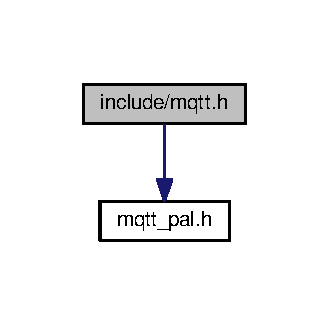
\includegraphics[width=350pt]{mqtt_8h__incl}
\end{center}
\end{figure}
\subsection*{Data Structures}
\begin{DoxyCompactItemize}
\item 
struct \hyperlink{structmqtt__fixed__header}{mqtt\+\_\+fixed\+\_\+header}
\begin{DoxyCompactList}\small\item\em The fixed header of an M\+Q\+TT control packet. \end{DoxyCompactList}\item 
struct \hyperlink{structmqtt__client}{mqtt\+\_\+client}
\begin{DoxyCompactList}\small\item\em An M\+Q\+TT client. \end{DoxyCompactList}\item 
struct \hyperlink{structmqtt__response__connack}{mqtt\+\_\+response\+\_\+connack}
\begin{DoxyCompactList}\small\item\em A connection response datastructure. \end{DoxyCompactList}\item 
struct \hyperlink{structmqtt__response__publish}{mqtt\+\_\+response\+\_\+publish}
\begin{DoxyCompactList}\small\item\em A publish packet received from the broker.

A publish packet is received from the broker when a client publishes to a topic that the {\itshape \{local} client\} is subscribed to. \end{DoxyCompactList}\item 
struct \hyperlink{structmqtt__response__puback}{mqtt\+\_\+response\+\_\+puback}
\begin{DoxyCompactList}\small\item\em A publish acknowledgement for messages that were published with QoS level 1. \end{DoxyCompactList}\item 
struct \hyperlink{structmqtt__response__pubrec}{mqtt\+\_\+response\+\_\+pubrec}
\begin{DoxyCompactList}\small\item\em The response packet to a P\+U\+B\+L\+I\+SH packet with QoS level 2. \end{DoxyCompactList}\item 
struct \hyperlink{structmqtt__response__pubrel}{mqtt\+\_\+response\+\_\+pubrel}
\begin{DoxyCompactList}\small\item\em The response to a P\+U\+B\+R\+EC packet. \end{DoxyCompactList}\item 
struct \hyperlink{structmqtt__response__pubcomp}{mqtt\+\_\+response\+\_\+pubcomp}
\begin{DoxyCompactList}\small\item\em The response to a P\+U\+B\+R\+EL packet. \end{DoxyCompactList}\item 
struct \hyperlink{structmqtt__response__suback}{mqtt\+\_\+response\+\_\+suback}
\begin{DoxyCompactList}\small\item\em The response to a subscription request. \end{DoxyCompactList}\item 
struct \hyperlink{structmqtt__response__unsuback}{mqtt\+\_\+response\+\_\+unsuback}
\begin{DoxyCompactList}\small\item\em The brokers response to a U\+N\+S\+U\+B\+S\+C\+R\+I\+BE request. \end{DoxyCompactList}\item 
struct \hyperlink{structmqtt__response__pingresp}{mqtt\+\_\+response\+\_\+pingresp}
\begin{DoxyCompactList}\small\item\em The response to a ping request. \end{DoxyCompactList}\item 
struct \hyperlink{structmqtt__response}{mqtt\+\_\+response}
\begin{DoxyCompactList}\small\item\em A struct used to deserialize/interpret an incoming packet from the broker. \end{DoxyCompactList}\end{DoxyCompactItemize}
\subsection*{Macros}
\begin{DoxyCompactItemize}
\item 
\#define \hyperlink{group__packers_ga50781ed232e8fd19a071d07566579974}{M\+Q\+T\+T\+\_\+\+P\+R\+O\+T\+O\+C\+O\+L\+\_\+\+L\+E\+V\+EL}~0x04
\begin{DoxyCompactList}\small\item\em The protocol identifier for M\+Q\+TT v3.\+1.\+1. \end{DoxyCompactList}\item 
\#define \hyperlink{mqtt_8h_a86c09e2666bd14722fa165ed904f78cb}{\+\_\+\+\_\+\+A\+L\+L\+\_\+\+M\+Q\+T\+T\+\_\+\+E\+R\+R\+O\+RS}(M\+Q\+T\+T\+\_\+\+E\+R\+R\+OR)
\begin{DoxyCompactList}\small\item\em A macro used to declare the enum Mqtt\+Errors and associated error messages (the members of the num) at the same time. \end{DoxyCompactList}\item 
\#define \hyperlink{mqtt_8h_aed8760364c7992625d06c93d12b2496d}{G\+E\+N\+E\+R\+A\+T\+E\+\_\+\+E\+N\+UM}(E\+N\+UM)~E\+N\+UM,
\begin{DoxyCompactList}\small\item\em A macro used to generate the enum Mqtt\+Errors from \hyperlink{mqtt_8h_a86c09e2666bd14722fa165ed904f78cb}{\+\_\+\+\_\+\+A\+L\+L\+\_\+\+M\+Q\+T\+T\+\_\+\+E\+R\+R\+O\+RS}. \end{DoxyCompactList}\item 
\#define \hyperlink{mqtt_8h_adf58d994c35f18ec84b628d8321f52e5}{G\+E\+N\+E\+R\+A\+T\+E\+\_\+\+S\+T\+R\+I\+NG}(S\+T\+R\+I\+NG)~\#S\+T\+R\+I\+NG,
\begin{DoxyCompactList}\small\item\em A macro used to generate the error messages associated with Mqtt\+Errors from \hyperlink{mqtt_8h_a86c09e2666bd14722fa165ed904f78cb}{\+\_\+\+\_\+\+A\+L\+L\+\_\+\+M\+Q\+T\+T\+\_\+\+E\+R\+R\+O\+RS}. \end{DoxyCompactList}\item 
\#define \hyperlink{mqtt_8h_a9f3be391755b744ee33832caf82b9749}{\+\_\+\+\_\+mqtt\+\_\+packed\+\_\+cstrlen}(x)~(2 + strlen(x))\hypertarget{mqtt_8h_a9f3be391755b744ee33832caf82b9749}{}\label{mqtt_8h_a9f3be391755b744ee33832caf82b9749}

\begin{DoxyCompactList}\small\item\em A macro to get the M\+Q\+TT string length from a c-\/string. \end{DoxyCompactList}\item 
\#define \hyperlink{group__packers_ga6501874871fce6b65d972430afa64fb8}{M\+Q\+T\+T\+\_\+\+S\+U\+B\+S\+C\+R\+I\+B\+E\+\_\+\+R\+E\+Q\+U\+E\+S\+T\+\_\+\+M\+A\+X\+\_\+\+N\+U\+M\+\_\+\+T\+O\+P\+I\+CS}~8
\begin{DoxyCompactList}\small\item\em The maximum number topics that can be subscribed to in a single call to mqtt\+\_\+pack\+\_\+subscribe\+\_\+request. \end{DoxyCompactList}\item 
\#define \hyperlink{group__packers_gaff4017b7a1668b6ad6e0d006d0fdf10e}{M\+Q\+T\+T\+\_\+\+U\+N\+S\+U\+B\+S\+C\+R\+I\+B\+E\+\_\+\+R\+E\+Q\+U\+E\+S\+T\+\_\+\+M\+A\+X\+\_\+\+N\+U\+M\+\_\+\+T\+O\+P\+I\+CS}~8
\begin{DoxyCompactList}\small\item\em The maximum number topics that can be subscribed to in a single call to mqtt\+\_\+pack\+\_\+unsubscribe\+\_\+request. \end{DoxyCompactList}\end{DoxyCompactItemize}
\subsection*{Enumerations}
\begin{DoxyCompactItemize}
\item 
enum \hyperlink{group__unpackers_gacbd36b88ec7f62bc161b07e1a0aed679}{M\+Q\+T\+T\+Control\+Packet\+Type} \{ \\*
{\bfseries M\+Q\+T\+T\+\_\+\+C\+O\+N\+T\+R\+O\+L\+\_\+\+C\+O\+N\+N\+E\+CT} =1u, 
{\bfseries M\+Q\+T\+T\+\_\+\+C\+O\+N\+T\+R\+O\+L\+\_\+\+C\+O\+N\+N\+A\+CK} =2u, 
{\bfseries M\+Q\+T\+T\+\_\+\+C\+O\+N\+T\+R\+O\+L\+\_\+\+P\+U\+B\+L\+I\+SH} =3u, 
{\bfseries M\+Q\+T\+T\+\_\+\+C\+O\+N\+T\+R\+O\+L\+\_\+\+P\+U\+B\+A\+CK} =4u, 
\\*
{\bfseries M\+Q\+T\+T\+\_\+\+C\+O\+N\+T\+R\+O\+L\+\_\+\+P\+U\+B\+R\+EC} =5u, 
{\bfseries M\+Q\+T\+T\+\_\+\+C\+O\+N\+T\+R\+O\+L\+\_\+\+P\+U\+B\+R\+EL} =6u, 
{\bfseries M\+Q\+T\+T\+\_\+\+C\+O\+N\+T\+R\+O\+L\+\_\+\+P\+U\+B\+C\+O\+MP} =7u, 
{\bfseries M\+Q\+T\+T\+\_\+\+C\+O\+N\+T\+R\+O\+L\+\_\+\+S\+U\+B\+S\+C\+R\+I\+BE} =8u, 
\\*
{\bfseries M\+Q\+T\+T\+\_\+\+C\+O\+N\+T\+R\+O\+L\+\_\+\+S\+U\+B\+A\+CK} =9u, 
{\bfseries M\+Q\+T\+T\+\_\+\+C\+O\+N\+T\+R\+O\+L\+\_\+\+U\+N\+S\+U\+B\+S\+C\+R\+I\+BE} =10u, 
{\bfseries M\+Q\+T\+T\+\_\+\+C\+O\+N\+T\+R\+O\+L\+\_\+\+U\+N\+S\+U\+B\+A\+CK} =11u, 
{\bfseries M\+Q\+T\+T\+\_\+\+C\+O\+N\+T\+R\+O\+L\+\_\+\+P\+I\+N\+G\+R\+EQ} =12u, 
\\*
{\bfseries M\+Q\+T\+T\+\_\+\+C\+O\+N\+T\+R\+O\+L\+\_\+\+P\+I\+N\+G\+R\+E\+SP} =13u, 
{\bfseries M\+Q\+T\+T\+\_\+\+C\+O\+N\+T\+R\+O\+L\+\_\+\+D\+I\+S\+C\+O\+N\+N\+E\+CT} =14u
 \}\begin{DoxyCompactList}\small\item\em An enumeration of the M\+Q\+TT control packet types. \end{DoxyCompactList}
\item 
enum \hyperlink{group__api_gabfef25ed21446904fd8b3a71cfa1f203}{Mqtt\+Errors} \{ \\*
{\bfseries M\+Q\+T\+T\+\_\+\+E\+R\+R\+O\+R\+\_\+\+U\+N\+K\+N\+O\+WN} =I\+N\+T\+\_\+\+M\+IN, 
{\bfseries M\+Q\+T\+T\+\_\+\+E\+R\+R\+O\+R\+\_\+\+N\+U\+L\+L\+P\+TR}, 
{\bfseries M\+Q\+T\+T\+\_\+\+E\+R\+R\+O\+R\+\_\+\+C\+O\+N\+T\+R\+O\+L\+\_\+\+F\+O\+R\+B\+I\+D\+D\+E\+N\+\_\+\+T\+Y\+PE}, 
{\bfseries M\+Q\+T\+T\+\_\+\+E\+R\+R\+O\+R\+\_\+\+C\+O\+N\+T\+R\+O\+L\+\_\+\+I\+N\+V\+A\+L\+I\+D\+\_\+\+F\+L\+A\+GS}, 
\\*
{\bfseries M\+Q\+T\+T\+\_\+\+E\+R\+R\+O\+R\+\_\+\+C\+O\+N\+T\+R\+O\+L\+\_\+\+W\+R\+O\+N\+G\+\_\+\+T\+Y\+PE}, 
{\bfseries M\+Q\+T\+T\+\_\+\+E\+R\+R\+O\+R\+\_\+\+C\+O\+N\+N\+E\+C\+T\+\_\+\+N\+U\+L\+L\+\_\+\+C\+L\+I\+E\+N\+T\+\_\+\+ID}, 
{\bfseries M\+Q\+T\+T\+\_\+\+E\+R\+R\+O\+R\+\_\+\+C\+O\+N\+N\+E\+C\+T\+\_\+\+N\+U\+L\+L\+\_\+\+W\+I\+L\+L\+\_\+\+M\+E\+S\+S\+A\+GE}, 
{\bfseries M\+Q\+T\+T\+\_\+\+E\+R\+R\+O\+R\+\_\+\+C\+O\+N\+N\+E\+C\+T\+\_\+\+F\+O\+R\+B\+I\+D\+D\+E\+N\+\_\+\+W\+I\+L\+L\+\_\+\+Q\+OS}, 
\\*
{\bfseries M\+Q\+T\+T\+\_\+\+E\+R\+R\+O\+R\+\_\+\+C\+O\+N\+N\+A\+C\+K\+\_\+\+F\+O\+R\+B\+I\+D\+D\+E\+N\+\_\+\+F\+L\+A\+GS}, 
{\bfseries M\+Q\+T\+T\+\_\+\+E\+R\+R\+O\+R\+\_\+\+C\+O\+N\+N\+A\+C\+K\+\_\+\+F\+O\+R\+B\+I\+D\+D\+E\+N\+\_\+\+C\+O\+DE}, 
{\bfseries M\+Q\+T\+T\+\_\+\+E\+R\+R\+O\+R\+\_\+\+P\+U\+B\+L\+I\+S\+H\+\_\+\+F\+O\+R\+B\+I\+D\+D\+E\+N\+\_\+\+Q\+OS}, 
{\bfseries M\+Q\+T\+T\+\_\+\+E\+R\+R\+O\+R\+\_\+\+S\+U\+B\+S\+C\+R\+I\+B\+E\+\_\+\+T\+O\+O\+\_\+\+M\+A\+N\+Y\+\_\+\+T\+O\+P\+I\+CS}, 
\\*
{\bfseries M\+Q\+T\+T\+\_\+\+E\+R\+R\+O\+R\+\_\+\+M\+A\+L\+F\+O\+R\+M\+E\+D\+\_\+\+R\+E\+S\+P\+O\+N\+SE}, 
{\bfseries M\+Q\+T\+T\+\_\+\+E\+R\+R\+O\+R\+\_\+\+U\+N\+S\+U\+B\+S\+C\+R\+I\+B\+E\+\_\+\+T\+O\+O\+\_\+\+M\+A\+N\+Y\+\_\+\+T\+O\+P\+I\+CS}, 
{\bfseries M\+Q\+T\+T\+\_\+\+E\+R\+R\+O\+R\+\_\+\+R\+E\+S\+P\+O\+N\+S\+E\+\_\+\+I\+N\+V\+A\+L\+I\+D\+\_\+\+C\+O\+N\+T\+R\+O\+L\+\_\+\+T\+Y\+PE}
 \}\begin{DoxyCompactList}\small\item\em An enumeration of error codes. Error messages can be retrieved by calling \hyperlink{group__api_ga6f0b3e9a177b03d5909e4f653fcd4038}{mqtt\+\_\+error\+\_\+str}. \end{DoxyCompactList}
\item 
enum \hyperlink{group__unpackers_ga07e480dfa5738e60c54ad0447ddb1a25}{M\+Q\+T\+T\+Connack\+Return\+Code} \{ \\*
{\bfseries M\+Q\+T\+T\+\_\+\+C\+O\+N\+N\+A\+C\+K\+\_\+\+A\+C\+C\+E\+P\+T\+ED} = 0u, 
{\bfseries M\+Q\+T\+T\+\_\+\+C\+O\+N\+N\+A\+C\+K\+\_\+\+R\+E\+F\+U\+S\+E\+D\+\_\+\+P\+R\+O\+T\+O\+C\+O\+L\+\_\+\+V\+E\+R\+S\+I\+ON} = 1u, 
{\bfseries M\+Q\+T\+T\+\_\+\+C\+O\+N\+N\+A\+C\+K\+\_\+\+R\+E\+F\+U\+S\+E\+D\+\_\+\+I\+D\+E\+N\+T\+I\+F\+I\+E\+R\+\_\+\+R\+E\+J\+E\+C\+T\+ED} = 2u, 
{\bfseries M\+Q\+T\+T\+\_\+\+C\+O\+N\+N\+A\+C\+K\+\_\+\+R\+E\+F\+U\+S\+E\+D\+\_\+\+S\+E\+R\+V\+E\+R\+\_\+\+U\+N\+A\+V\+A\+I\+L\+A\+B\+LE} = 3u, 
\\*
{\bfseries M\+Q\+T\+T\+\_\+\+C\+O\+N\+N\+A\+C\+K\+\_\+\+R\+E\+F\+U\+S\+E\+D\+\_\+\+B\+A\+D\+\_\+\+U\+S\+E\+R\+\_\+\+N\+A\+M\+E\+\_\+\+O\+R\+\_\+\+P\+A\+S\+S\+W\+O\+RD} = 4u, 
{\bfseries M\+Q\+T\+T\+\_\+\+C\+O\+N\+N\+A\+C\+K\+\_\+\+R\+E\+F\+U\+S\+E\+D\+\_\+\+N\+O\+T\+\_\+\+A\+U\+T\+H\+O\+R\+I\+Z\+ED} = 5u
 \}\begin{DoxyCompactList}\small\item\em An enumeration of the return codes returned in a C\+O\+N\+N\+A\+CK packet. \end{DoxyCompactList}
\item 
enum \hyperlink{group__unpackers_ga2d626b05e589a148ce2e9e97f41302ae}{M\+Q\+T\+T\+Suback\+Return\+Codes} \{ {\bfseries M\+Q\+T\+T\+\_\+\+S\+U\+B\+A\+C\+K\+\_\+\+S\+U\+C\+C\+E\+S\+S\+\_\+\+M\+A\+X\+\_\+\+Q\+O\+S\+\_\+0} = 0u, 
{\bfseries M\+Q\+T\+T\+\_\+\+S\+U\+B\+A\+C\+K\+\_\+\+S\+U\+C\+C\+E\+S\+S\+\_\+\+M\+A\+X\+\_\+\+Q\+O\+S\+\_\+1} = 1u, 
{\bfseries M\+Q\+T\+T\+\_\+\+S\+U\+B\+A\+C\+K\+\_\+\+S\+U\+C\+C\+E\+S\+S\+\_\+\+M\+A\+X\+\_\+\+Q\+O\+S\+\_\+2} = 2u, 
{\bfseries M\+Q\+T\+T\+\_\+\+S\+U\+B\+A\+C\+K\+\_\+\+F\+A\+I\+L\+U\+RE} = 128u
 \}\begin{DoxyCompactList}\small\item\em An enumeration of subscription acknowledgement return codes. \end{DoxyCompactList}
\item 
enum \hyperlink{group__packers_gad6fa84a96a940fe4eae6ffca1a6d945f}{M\+Q\+T\+T\+Connect\+Flags} \{ \\*
{\bfseries M\+Q\+T\+T\+\_\+\+C\+O\+N\+N\+E\+C\+T\+\_\+\+R\+E\+S\+E\+R\+V\+ED} = 1u, 
{\bfseries M\+Q\+T\+T\+\_\+\+C\+O\+N\+N\+E\+C\+T\+\_\+\+C\+L\+E\+A\+N\+\_\+\+S\+E\+S\+S\+I\+ON} = 2u, 
{\bfseries M\+Q\+T\+T\+\_\+\+C\+O\+N\+N\+E\+C\+T\+\_\+\+W\+I\+L\+L\+\_\+\+F\+L\+AG} = 4u, 
{\bfseries M\+Q\+T\+T\+\_\+\+C\+O\+N\+N\+E\+C\+T\+\_\+\+W\+I\+L\+L\+\_\+\+Q\+O\+S\+\_\+0} = (0u \& 0x03) $<$$<$ 3, 
\\*
{\bfseries M\+Q\+T\+T\+\_\+\+C\+O\+N\+N\+E\+C\+T\+\_\+\+W\+I\+L\+L\+\_\+\+Q\+O\+S\+\_\+1} = (1u \& 0x03) $<$$<$ 3, 
{\bfseries M\+Q\+T\+T\+\_\+\+C\+O\+N\+N\+E\+C\+T\+\_\+\+W\+I\+L\+L\+\_\+\+Q\+O\+S\+\_\+2} = (2u \& 0x03) $<$$<$ 3, 
{\bfseries M\+Q\+T\+T\+\_\+\+C\+O\+N\+N\+E\+C\+T\+\_\+\+W\+I\+L\+L\+\_\+\+R\+E\+T\+A\+IN} = 32u, 
{\bfseries M\+Q\+T\+T\+\_\+\+C\+O\+N\+N\+E\+C\+T\+\_\+\+P\+A\+S\+S\+W\+O\+RD} = 64u, 
\\*
{\bfseries M\+Q\+T\+T\+\_\+\+C\+O\+N\+N\+E\+C\+T\+\_\+\+U\+S\+E\+R\+\_\+\+N\+A\+ME} = 128u
 \}\begin{DoxyCompactList}\small\item\em An enumeration of C\+O\+N\+N\+E\+CT packet flags. \end{DoxyCompactList}
\item 
enum \hyperlink{group__packers_gad38a41e1c497f9bcd2477c005f280b23}{M\+Q\+T\+T\+Publish\+Flags} \{ \\*
{\bfseries M\+Q\+T\+T\+\_\+\+P\+U\+B\+L\+I\+S\+H\+\_\+\+D\+UP} = 8u, 
{\bfseries M\+Q\+T\+T\+\_\+\+P\+U\+B\+L\+I\+S\+H\+\_\+\+Q\+O\+S\+\_\+0} = ((0u $<$$<$ 1) \& 0x06), 
{\bfseries M\+Q\+T\+T\+\_\+\+P\+U\+B\+L\+I\+S\+H\+\_\+\+Q\+O\+S\+\_\+1} = ((1u $<$$<$ 1) \& 0x06), 
{\bfseries M\+Q\+T\+T\+\_\+\+P\+U\+B\+L\+I\+S\+H\+\_\+\+Q\+O\+S\+\_\+2} = ((2u $<$$<$ 1) \& 0x06), 
\\*
{\bfseries M\+Q\+T\+T\+\_\+\+P\+U\+B\+L\+I\+S\+H\+\_\+\+R\+E\+T\+A\+IN} = 0x01
 \}\begin{DoxyCompactList}\small\item\em An enumeration of the P\+U\+B\+L\+I\+SH flags. \end{DoxyCompactList}
\end{DoxyCompactItemize}
\subsection*{Functions}
\begin{DoxyCompactItemize}
\item 
const char $\ast$ \hyperlink{group__api_ga6f0b3e9a177b03d5909e4f653fcd4038}{mqtt\+\_\+error\+\_\+str} (enum \hyperlink{group__api_gabfef25ed21446904fd8b3a71cfa1f203}{Mqtt\+Errors} error)
\begin{DoxyCompactList}\small\item\em Returns an error message for error code, {\ttfamily error}. \end{DoxyCompactList}\item 
ssize\+\_\+t \hyperlink{mqtt_8h_a223d30d2e6b84824ed995eda885d1e5d}{\+\_\+\+\_\+mqtt\+\_\+pack\+\_\+str} (uint8\+\_\+t $\ast$buf, const char $\ast$str)
\begin{DoxyCompactList}\small\item\em Pack a M\+Q\+TT string, given a c-\/string {\ttfamily str}. \end{DoxyCompactList}\item 
ssize\+\_\+t \hyperlink{group__unpackers_gad596aa5faf7f79e05fb15da33321db10}{mqtt\+\_\+unpack\+\_\+fixed\+\_\+header} (struct \hyperlink{structmqtt__response}{mqtt\+\_\+response} $\ast$response, const uint8\+\_\+t $\ast$buf, size\+\_\+t bufsz)
\begin{DoxyCompactList}\small\item\em Deserialize the contents of {\ttfamily buf} into an \hyperlink{structmqtt__fixed__header}{mqtt\+\_\+fixed\+\_\+header} object. \end{DoxyCompactList}\item 
ssize\+\_\+t \hyperlink{group__packers_ga52d369e6e7d44539aab6732375288623}{mqtt\+\_\+pack\+\_\+fixed\+\_\+header} (uint8\+\_\+t $\ast$buf, size\+\_\+t bufsz, const struct \hyperlink{structmqtt__fixed__header}{mqtt\+\_\+fixed\+\_\+header} $\ast$fixed\+\_\+header)
\begin{DoxyCompactList}\small\item\em Serialize an \hyperlink{structmqtt__fixed__header}{mqtt\+\_\+fixed\+\_\+header} and write it to {\ttfamily buf}. \end{DoxyCompactList}\item 
ssize\+\_\+t \hyperlink{group__packers_ga0ed22cd47cf955e07e9662f1d9a4989c}{mqtt\+\_\+pack\+\_\+connection\+\_\+request} (uint8\+\_\+t $\ast$buf, size\+\_\+t bufsz, const char $\ast$client\+\_\+id, const char $\ast$will\+\_\+topic, const char $\ast$will\+\_\+message, const char $\ast$user\+\_\+name, const char $\ast$password, uint8\+\_\+t connect\+\_\+flags, uint16\+\_\+t keep\+\_\+alive)
\begin{DoxyCompactList}\small\item\em Serialize a connection request into a buffer. \end{DoxyCompactList}\item 
ssize\+\_\+t \hyperlink{group__packers_gae7cb4c4d90ed04fe268f5f9a167e32b1}{mqtt\+\_\+pack\+\_\+publish\+\_\+request} (uint8\+\_\+t $\ast$buf, size\+\_\+t bufsz, const char $\ast$topic\+\_\+name, uint16\+\_\+t packet\+\_\+id, void $\ast$application\+\_\+message, size\+\_\+t application\+\_\+message\+\_\+size, uint8\+\_\+t publish\+\_\+flags)
\begin{DoxyCompactList}\small\item\em Serialize a P\+U\+B\+L\+I\+SH request and put it in {\ttfamily buf}. \end{DoxyCompactList}\item 
ssize\+\_\+t \hyperlink{group__packers_ga9cbd954d6bffd8fb0a06a6e4d34e4949}{mqtt\+\_\+pack\+\_\+pubxxx\+\_\+request} (uint8\+\_\+t $\ast$buf, size\+\_\+t bufsz, enum \hyperlink{group__unpackers_gacbd36b88ec7f62bc161b07e1a0aed679}{M\+Q\+T\+T\+Control\+Packet\+Type} control\+\_\+type, uint16\+\_\+t packet\+\_\+id)
\begin{DoxyCompactList}\small\item\em Serialize a P\+U\+B\+A\+CK, P\+U\+B\+R\+EC, P\+U\+B\+R\+EL, or P\+U\+B\+C\+O\+MP packet and put it in {\ttfamily buf}. \end{DoxyCompactList}\item 
ssize\+\_\+t \hyperlink{group__packers_ga65a198063d780e654af0336e5088f609}{mqtt\+\_\+pack\+\_\+subscribe\+\_\+request} (uint8\+\_\+t $\ast$buf, size\+\_\+t bufsz, uint16\+\_\+t packet\+\_\+id,...)
\begin{DoxyCompactList}\small\item\em Serialize a S\+U\+B\+S\+C\+R\+I\+BE packet and put it in {\ttfamily buf}. \end{DoxyCompactList}\item 
ssize\+\_\+t \hyperlink{group__packers_ga3a0e5c05084d708f16cb1a244cbcaad5}{mqtt\+\_\+pack\+\_\+unsubscribe\+\_\+request} (uint8\+\_\+t $\ast$buf, size\+\_\+t bufsz, uint16\+\_\+t packet\+\_\+id,...)
\begin{DoxyCompactList}\small\item\em Serialize a U\+N\+S\+U\+B\+S\+C\+R\+I\+BE packet and put it in {\ttfamily buf}. \end{DoxyCompactList}\item 
ssize\+\_\+t \hyperlink{group__packers_gac11b5cc5c6bbbf386c2515c823965a82}{mqtt\+\_\+pack\+\_\+ping\+\_\+request} (uint8\+\_\+t $\ast$buf, size\+\_\+t bufsz)
\begin{DoxyCompactList}\small\item\em Serialize a P\+I\+N\+G\+R\+EQ and put it into {\ttfamily buf}. \end{DoxyCompactList}\item 
ssize\+\_\+t \hyperlink{group__packers_ga7842c85a0711df31f2e9ce31a9253999}{mqtt\+\_\+pack\+\_\+disconnect} (uint8\+\_\+t $\ast$buf, size\+\_\+t bufsz)
\begin{DoxyCompactList}\small\item\em Serialize a D\+I\+S\+C\+O\+N\+N\+E\+CT and put it into {\ttfamily buf}. \end{DoxyCompactList}\end{DoxyCompactItemize}


\subsection{Macro Definition Documentation}
\index{mqtt.\+h@{mqtt.\+h}!\+\_\+\+\_\+\+A\+L\+L\+\_\+\+M\+Q\+T\+T\+\_\+\+E\+R\+R\+O\+RS@{\+\_\+\+\_\+\+A\+L\+L\+\_\+\+M\+Q\+T\+T\+\_\+\+E\+R\+R\+O\+RS}}
\index{\+\_\+\+\_\+\+A\+L\+L\+\_\+\+M\+Q\+T\+T\+\_\+\+E\+R\+R\+O\+RS@{\+\_\+\+\_\+\+A\+L\+L\+\_\+\+M\+Q\+T\+T\+\_\+\+E\+R\+R\+O\+RS}!mqtt.\+h@{mqtt.\+h}}
\subsubsection[{\texorpdfstring{\+\_\+\+\_\+\+A\+L\+L\+\_\+\+M\+Q\+T\+T\+\_\+\+E\+R\+R\+O\+RS}{__ALL_MQTT_ERRORS}}]{\setlength{\rightskip}{0pt plus 5cm}\#define \+\_\+\+\_\+\+A\+L\+L\+\_\+\+M\+Q\+T\+T\+\_\+\+E\+R\+R\+O\+RS(
\begin{DoxyParamCaption}
\item[{}]{M\+Q\+T\+T\+\_\+\+E\+R\+R\+OR}
\end{DoxyParamCaption}
)}\hypertarget{mqtt_8h_a86c09e2666bd14722fa165ed904f78cb}{}\label{mqtt_8h_a86c09e2666bd14722fa165ed904f78cb}
{\bfseries Value\+:}
\begin{DoxyCode}
MQTT\_ERROR(MQTT\_ERROR\_NULLPTR)                       \(\backslash\)
    MQTT\_ERROR(MQTT\_ERROR\_CONTROL\_FORBIDDEN\_TYPE)        \(\backslash\)
    MQTT\_ERROR(MQTT\_ERROR\_CONTROL\_INVALID\_FLAGS)         \(\backslash\)
    MQTT\_ERROR(MQTT\_ERROR\_CONTROL\_WRONG\_TYPE)            \(\backslash\)
    MQTT\_ERROR(MQTT\_ERROR\_CONNECT\_NULL\_CLIENT\_ID)        \(\backslash\)
    MQTT\_ERROR(MQTT\_ERROR\_CONNECT\_NULL\_WILL\_MESSAGE)     \(\backslash\)
    MQTT\_ERROR(MQTT\_ERROR\_CONNECT\_FORBIDDEN\_WILL\_QOS)    \(\backslash\)
    MQTT\_ERROR(MQTT\_ERROR\_CONNACK\_FORBIDDEN\_FLAGS)       \(\backslash\)
    MQTT\_ERROR(MQTT\_ERROR\_CONNACK\_FORBIDDEN\_CODE)        \(\backslash\)
    MQTT\_ERROR(MQTT\_ERROR\_PUBLISH\_FORBIDDEN\_QOS)         \(\backslash\)
    MQTT\_ERROR(MQTT\_ERROR\_SUBSCRIBE\_TOO\_MANY\_TOPICS)     \(\backslash\)
    MQTT\_ERROR(MQTT\_ERROR\_MALFORMED\_RESPONSE)            \(\backslash\)
    MQTT\_ERROR(MQTT\_ERROR\_UNSUBSCRIBE\_TOO\_MANY\_TOPICS)   \(\backslash\)
    MQTT\_ERROR(MQTT\_ERROR\_RESPONSE\_INVALID\_CONTROL\_TYPE) \(\backslash\)
\end{DoxyCode}


A macro used to declare the enum Mqtt\+Errors and associated error messages (the members of the num) at the same time. 

\index{mqtt.\+h@{mqtt.\+h}!G\+E\+N\+E\+R\+A\+T\+E\+\_\+\+E\+N\+UM@{G\+E\+N\+E\+R\+A\+T\+E\+\_\+\+E\+N\+UM}}
\index{G\+E\+N\+E\+R\+A\+T\+E\+\_\+\+E\+N\+UM@{G\+E\+N\+E\+R\+A\+T\+E\+\_\+\+E\+N\+UM}!mqtt.\+h@{mqtt.\+h}}
\subsubsection[{\texorpdfstring{G\+E\+N\+E\+R\+A\+T\+E\+\_\+\+E\+N\+UM}{GENERATE_ENUM}}]{\setlength{\rightskip}{0pt plus 5cm}\#define G\+E\+N\+E\+R\+A\+T\+E\+\_\+\+E\+N\+UM(
\begin{DoxyParamCaption}
\item[{}]{E\+N\+UM}
\end{DoxyParamCaption}
)~E\+N\+UM,}\hypertarget{mqtt_8h_aed8760364c7992625d06c93d12b2496d}{}\label{mqtt_8h_aed8760364c7992625d06c93d12b2496d}


A macro used to generate the enum Mqtt\+Errors from \hyperlink{mqtt_8h_a86c09e2666bd14722fa165ed904f78cb}{\+\_\+\+\_\+\+A\+L\+L\+\_\+\+M\+Q\+T\+T\+\_\+\+E\+R\+R\+O\+RS}. 

\begin{DoxySeeAlso}{See also}
\hyperlink{mqtt_8h_a86c09e2666bd14722fa165ed904f78cb}{\+\_\+\+\_\+\+A\+L\+L\+\_\+\+M\+Q\+T\+T\+\_\+\+E\+R\+R\+O\+RS} 
\end{DoxySeeAlso}
\index{mqtt.\+h@{mqtt.\+h}!G\+E\+N\+E\+R\+A\+T\+E\+\_\+\+S\+T\+R\+I\+NG@{G\+E\+N\+E\+R\+A\+T\+E\+\_\+\+S\+T\+R\+I\+NG}}
\index{G\+E\+N\+E\+R\+A\+T\+E\+\_\+\+S\+T\+R\+I\+NG@{G\+E\+N\+E\+R\+A\+T\+E\+\_\+\+S\+T\+R\+I\+NG}!mqtt.\+h@{mqtt.\+h}}
\subsubsection[{\texorpdfstring{G\+E\+N\+E\+R\+A\+T\+E\+\_\+\+S\+T\+R\+I\+NG}{GENERATE_STRING}}]{\setlength{\rightskip}{0pt plus 5cm}\#define G\+E\+N\+E\+R\+A\+T\+E\+\_\+\+S\+T\+R\+I\+NG(
\begin{DoxyParamCaption}
\item[{}]{S\+T\+R\+I\+NG}
\end{DoxyParamCaption}
)~\#S\+T\+R\+I\+NG,}\hypertarget{mqtt_8h_adf58d994c35f18ec84b628d8321f52e5}{}\label{mqtt_8h_adf58d994c35f18ec84b628d8321f52e5}


A macro used to generate the error messages associated with Mqtt\+Errors from \hyperlink{mqtt_8h_a86c09e2666bd14722fa165ed904f78cb}{\+\_\+\+\_\+\+A\+L\+L\+\_\+\+M\+Q\+T\+T\+\_\+\+E\+R\+R\+O\+RS}. 

\begin{DoxySeeAlso}{See also}
\hyperlink{mqtt_8h_a86c09e2666bd14722fa165ed904f78cb}{\+\_\+\+\_\+\+A\+L\+L\+\_\+\+M\+Q\+T\+T\+\_\+\+E\+R\+R\+O\+RS} 
\end{DoxySeeAlso}


\subsection{Function Documentation}
\index{mqtt.\+h@{mqtt.\+h}!\+\_\+\+\_\+mqtt\+\_\+pack\+\_\+str@{\+\_\+\+\_\+mqtt\+\_\+pack\+\_\+str}}
\index{\+\_\+\+\_\+mqtt\+\_\+pack\+\_\+str@{\+\_\+\+\_\+mqtt\+\_\+pack\+\_\+str}!mqtt.\+h@{mqtt.\+h}}
\subsubsection[{\texorpdfstring{\+\_\+\+\_\+mqtt\+\_\+pack\+\_\+str(uint8\+\_\+t $\ast$buf, const char $\ast$str)}{__mqtt_pack_str(uint8_t *buf, const char *str)}}]{\setlength{\rightskip}{0pt plus 5cm}ssize\+\_\+t \+\_\+\+\_\+mqtt\+\_\+pack\+\_\+str (
\begin{DoxyParamCaption}
\item[{uint8\+\_\+t $\ast$}]{buf, }
\item[{const char $\ast$}]{str}
\end{DoxyParamCaption}
)}\hypertarget{mqtt_8h_a223d30d2e6b84824ed995eda885d1e5d}{}\label{mqtt_8h_a223d30d2e6b84824ed995eda885d1e5d}


Pack a M\+Q\+TT string, given a c-\/string {\ttfamily str}. 


\begin{DoxyParams}[1]{Parameters}
\mbox{\tt out}  & {\em buf} & the buffer that the M\+Q\+TT string will be written to. \\
\hline
\mbox{\tt in}  & {\em str} & the c-\/string to be written to {\ttfamily buf}.\\
\hline
\end{DoxyParams}
\begin{DoxyWarning}{Warning}
This function provides no error checking.
\end{DoxyWarning}
\begin{DoxyReturn}{Returns}
strlen(str) + 2 
\end{DoxyReturn}

\hypertarget{mqtt__pal_8h}{}\section{include/mqtt\+\_\+pal.h File Reference}
\label{mqtt__pal_8h}\index{include/mqtt\+\_\+pal.\+h@{include/mqtt\+\_\+pal.\+h}}


Includes/supports the types/calls required by the M\+Q\+T\+T-\/C client.  


This graph shows which files directly or indirectly include this file\+:\nopagebreak
\begin{figure}[H]
\begin{center}
\leavevmode
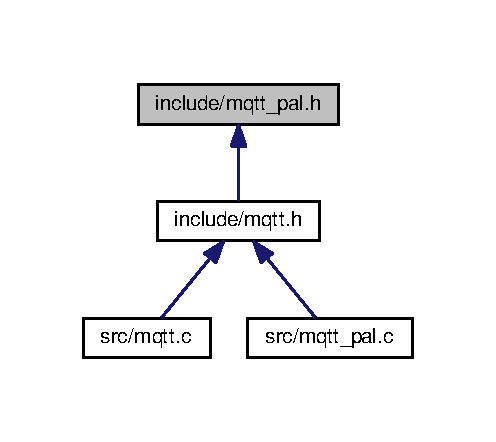
\includegraphics[width=238pt]{mqtt__pal_8h__dep__incl}
\end{center}
\end{figure}
\subsection*{Functions}
\begin{DoxyCompactItemize}
\item 
ssize\+\_\+t \hyperlink{group__pal_gac8dd7d5af889f5933dda733007adb9a3}{mqtt\+\_\+pal\+\_\+sendall} (int fd, const void $\ast$buf, size\+\_\+t len, int flags)
\begin{DoxyCompactList}\small\item\em Sends all the bytes in a buffer. \end{DoxyCompactList}\item 
ssize\+\_\+t \hyperlink{group__pal_ga620d6ab20694c9b4d99293a47491004e}{mqtt\+\_\+pal\+\_\+recvall} (int fd, void $\ast$buf, size\+\_\+t bufsz, int flags)
\begin{DoxyCompactList}\small\item\em Non-\/blocking receive all the byte available. \end{DoxyCompactList}\end{DoxyCompactItemize}


\subsection{Detailed Description}
Includes/supports the types/calls required by the M\+Q\+T\+T-\/C client. 

\begin{DoxyNote}{Note}
This is the {\itshape only} file included in \hyperlink{mqtt_8h}{mqtt.\+h}, and \hyperlink{mqtt_8c}{mqtt.\+c}. It is therefore responsible for including/supporting all the required types and calls. 
\end{DoxyNote}

\hypertarget{mqtt_8c}{}\section{src/mqtt.c File Reference}
\label{mqtt_8c}\index{src/mqtt.\+c@{src/mqtt.\+c}}


Implements the functionality of M\+Q\+T\+T-\/C.  


{\ttfamily \#include $<$mqtt.\+h$>$}\\*
Include dependency graph for mqtt.\+c\+:\nopagebreak
\begin{figure}[H]
\begin{center}
\leavevmode
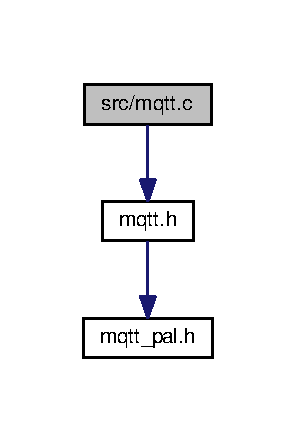
\includegraphics[width=142pt]{mqtt_8c__incl}
\end{center}
\end{figure}


\subsection{Detailed Description}
Implements the functionality of M\+Q\+T\+T-\/C. 

\begin{DoxyNote}{Note}
The only files that are included are \hyperlink{mqtt_8h}{mqtt.\+h} and \hyperlink{mqtt__pal_8h}{mqtt\+\_\+pal.\+h}. 
\end{DoxyNote}

\hypertarget{mqtt__pal_8c}{}\section{src/mqtt\+\_\+pal.c File Reference}
\label{mqtt__pal_8c}\index{src/mqtt\+\_\+pal.\+c@{src/mqtt\+\_\+pal.\+c}}


Implements \hyperlink{group__pal_gac8dd7d5af889f5933dda733007adb9a3}{mqtt\+\_\+pal\+\_\+sendall} and \hyperlink{group__pal_ga620d6ab20694c9b4d99293a47491004e}{mqtt\+\_\+pal\+\_\+recvall} and any platform-\/specific helpers you\textquotesingle{}d like.  


{\ttfamily \#include $<$mqtt.\+h$>$}\\*
Include dependency graph for mqtt\+\_\+pal.\+c\+:\nopagebreak
\begin{figure}[H]
\begin{center}
\leavevmode
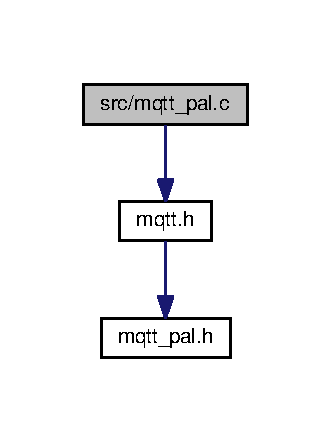
\includegraphics[width=159pt]{mqtt__pal_8c__incl}
\end{center}
\end{figure}


\subsection{Detailed Description}
Implements \hyperlink{group__pal_gac8dd7d5af889f5933dda733007adb9a3}{mqtt\+\_\+pal\+\_\+sendall} and \hyperlink{group__pal_ga620d6ab20694c9b4d99293a47491004e}{mqtt\+\_\+pal\+\_\+recvall} and any platform-\/specific helpers you\textquotesingle{}d like. 


\chapter{Example Documentation}
\hypertarget{simple_publisher_8c-example}{}\section{simple\+\_\+publisher.\+c}
A simple program to that publishes the current time whenever E\+N\+T\+ER is pressed.

Usage\+: 
\begin{DoxyCode}
1 ./simple\_publisher [address [port [topic]]]
\end{DoxyCode}


Where {\ttfamily address} is the address of the M\+Q\+TT broker, {\ttfamily port} it the port number the M\+Q\+TT broker is running on, and {\ttfamily topic} is the name of the topic to P\+U\+B\+L\+I\+SH times to. Note that all these arguments are optional and the defaults are {\ttfamily address} = {\ttfamily \char`\"{}test.\+mosquitto.\+org\char`\"{}}, {\ttfamily port} = {\ttfamily \char`\"{}1883\char`\"{}}, and {\ttfamily topic} = \char`\"{}datetime\char`\"{}.


\begin{DoxyCodeInclude}

\textcolor{preprocessor}{#include <unistd.h>}
\textcolor{preprocessor}{#include <stdlib.h>}
\textcolor{preprocessor}{#include <stdio.h>}

\textcolor{preprocessor}{#include <\hyperlink{mqtt_8h}{mqtt.h}>}


\textcolor{keywordtype}{void} publish\_callback(\textcolor{keywordtype}{void}** unused, \textcolor{keyword}{struct} \hyperlink{structmqtt__response__publish}{mqtt\_response\_publish} *published);

\textcolor{keywordtype}{void}* client\_refresher(\textcolor{keywordtype}{void}* client);

\textcolor{keywordtype}{void} exit\_example(\textcolor{keywordtype}{int} status, \textcolor{keywordtype}{int} sockfd, pthread\_t *client\_daemon);

\textcolor{keywordtype}{int} main(\textcolor{keywordtype}{int} argc, \textcolor{keyword}{const} \textcolor{keywordtype}{char} *argv[]) 
\{
    \textcolor{keyword}{const} \textcolor{keywordtype}{char}* addr;
    \textcolor{keyword}{const} \textcolor{keywordtype}{char}* port;
    \textcolor{keyword}{const} \textcolor{keywordtype}{char}* topic;

    \textcolor{comment}{/* get address (argv[1] if present) */}
    \textcolor{keywordflow}{if} (argc > 1) \{
        addr = argv[1];
    \} \textcolor{keywordflow}{else} \{
        addr = \textcolor{stringliteral}{"test.mosquitto.org"};
    \}

    \textcolor{comment}{/* get port number (argv[2] if present) */}
    \textcolor{keywordflow}{if} (argc > 2) \{
        port = argv[2];
    \} \textcolor{keywordflow}{else} \{
        port = \textcolor{stringliteral}{"1883"};
    \}

    \textcolor{comment}{/* get the topic name to publish */}
    \textcolor{keywordflow}{if} (argc > 3) \{
        topic = argv[3];
    \} \textcolor{keywordflow}{else} \{
        topic = \textcolor{stringliteral}{"datetime"};
    \}

    \textcolor{comment}{/* open the non-blocking TCP socket (connecting to the broker) */}
    \textcolor{keywordtype}{int} sockfd = mqtt\_pal\_sockopen(addr, port, AF\_INET);

    \textcolor{keywordflow}{if} (sockfd == -1) \{
        perror(\textcolor{stringliteral}{"Failed to open socket: "});
        exit\_example(EXIT\_FAILURE, sockfd, NULL);
    \}

    \textcolor{comment}{/* setup a client */}
    \textcolor{keyword}{struct }\hyperlink{structmqtt__client}{mqtt\_client} client;
    uint8\_t sendbuf[2048]; \textcolor{comment}{/* sendbuf should be large enough to hold multiple whole mqtt messages */}
    uint8\_t recvbuf[1024]; \textcolor{comment}{/* recvbuf should be large enough any whole mqtt message expected to be received
       */}
    \hyperlink{group__api_gab07105b049dd86a8ec39c518cf9fa4c7}{mqtt\_init}(&client, sockfd, sendbuf, \textcolor{keyword}{sizeof}(sendbuf), recvbuf, \textcolor{keyword}{sizeof}(recvbuf), 
      publish\_callback);
    \hyperlink{group__api_gadbe914e5a9d4f93314c4e7637cb4f7b3}{mqtt\_connect}(&client, \textcolor{stringliteral}{"publishing\_client"}, NULL, NULL, 0, NULL, NULL, 0, 400);

    \textcolor{comment}{/* check that we don't have any errors */}
    \textcolor{keywordflow}{if} (client.error != MQTT\_OK) \{
        fprintf(stderr, \textcolor{stringliteral}{"error: %s\(\backslash\)n"}, \hyperlink{group__api_ga47b62bdd24e8b05957825d2419d7c848}{mqtt\_error\_str}(client.error));
        exit\_example(EXIT\_FAILURE, sockfd, NULL);
    \}

    \textcolor{comment}{/* start a thread to refresh the client (handle egress and ingree client traffic) */}
    pthread\_t client\_daemon;
    \textcolor{keywordflow}{if}(pthread\_create(&client\_daemon, NULL, client\_refresher, &client)) \{
        fprintf(stderr, \textcolor{stringliteral}{"Failed to start client daemon.\(\backslash\)n"});
        exit\_example(EXIT\_FAILURE, sockfd, NULL);

    \}

    \textcolor{comment}{/* start publishing the time */}
    printf(\textcolor{stringliteral}{"%s is ready to begin publishing the time.\(\backslash\)n"}, argv[0]);
    printf(\textcolor{stringliteral}{"Press ENTER to publish the current time.\(\backslash\)n"});
    printf(\textcolor{stringliteral}{"Press CTRL-D (or any other key) to exit.\(\backslash\)n\(\backslash\)n"});
    \textcolor{keywordflow}{while}(fgetc(stdin) == \textcolor{charliteral}{'\(\backslash\)n'}) \{
        \textcolor{comment}{/* get the current time */}
        time\_t timer;
        time(&timer);
        \textcolor{keyword}{struct }tm* tm\_info = localtime(&timer);
        \textcolor{keywordtype}{char} timebuf[26];
        strftime(timebuf, 26, \textcolor{stringliteral}{"%Y-%m-%d %H:%M:%S"}, tm\_info);

        \textcolor{comment}{/* print a message */}
        \textcolor{keywordtype}{char} application\_message[256];
        snprintf(application\_message, \textcolor{keyword}{sizeof}(application\_message), \textcolor{stringliteral}{"The time is %s"}, timebuf);
        printf(\textcolor{stringliteral}{"%s published : \(\backslash\)"%s\(\backslash\)""}, argv[0], application\_message);

        \textcolor{comment}{/* publish the time */}
        \hyperlink{group__api_ga0d8fed24a799ab9b55eeb28f3cd2d0a8}{mqtt\_publish}(&client, topic, application\_message, strlen(application\_message) + 1, 
      MQTT\_PUBLISH\_QOS\_0);

        \textcolor{comment}{/* check for errors */}
        \textcolor{keywordflow}{if} (client.error != MQTT\_OK) \{
            fprintf(stderr, \textcolor{stringliteral}{"error: %s\(\backslash\)n"}, \hyperlink{group__api_ga47b62bdd24e8b05957825d2419d7c848}{mqtt\_error\_str}(client.error));
            exit\_example(EXIT\_FAILURE, sockfd, &client\_daemon);
        \}
    \}   

    \textcolor{comment}{/* disconnect */}
    printf(\textcolor{stringliteral}{"\(\backslash\)n%s disconnecting from %s\(\backslash\)n"}, argv[0], addr);
    sleep(1);

    \textcolor{comment}{/* exit */} 
    exit\_example(EXIT\_SUCCESS, sockfd, &client\_daemon);
\}

\textcolor{keywordtype}{void} exit\_example(\textcolor{keywordtype}{int} status, \textcolor{keywordtype}{int} sockfd, pthread\_t *client\_daemon)
\{
    \textcolor{keywordflow}{if} (sockfd != -1) close(sockfd);
    \textcolor{keywordflow}{if} (client\_daemon != NULL) pthread\_cancel(*client\_daemon);
    exit(status);
\}



\textcolor{keywordtype}{void} publish\_callback(\textcolor{keywordtype}{void}** unused, \textcolor{keyword}{struct} \hyperlink{structmqtt__response__publish}{mqtt\_response\_publish} *published) 
\{
    \textcolor{comment}{/* not used in this example */}
\}

\textcolor{keywordtype}{void}* client\_refresher(\textcolor{keywordtype}{void}* client)
\{
    \textcolor{keywordflow}{while}(1) 
    \{
        \hyperlink{group__api_gae3d3aafc7588ed53a90c9f66fc620a6e}{mqtt\_sync}((\textcolor{keyword}{struct} \hyperlink{structmqtt__client}{mqtt\_client}*) client);
        usleep(100000U);
    \}
    \textcolor{keywordflow}{return} NULL;
\}
\end{DoxyCodeInclude}
 
\hypertarget{simple_subscriber_8c-example}{}\section{simple\+\_\+subscriber.\+c}
A simple program that subscribes to a single topic and prints all updates that are received.

Usage\+: 
\begin{DoxyCode}
1 ./bin/simple\_subscriber [address [port [topic]]]
\end{DoxyCode}


Where {\ttfamily address} is the address of the M\+Q\+TT broker, {\ttfamily port} is the port number the M\+Q\+TT broker is running on, and {\ttfamily topic} is the name of the topic subscribe to. Note that all these arguments are optional and the defaults are {\ttfamily address} = {\ttfamily \char`\"{}test.\+mosquitto.\+org\char`\"{}}, {\ttfamily port} = {\ttfamily \char`\"{}1883\char`\"{}}, and {\ttfamily topic} = \char`\"{}datetime\char`\"{}.


\begin{DoxyCodeInclude}

\textcolor{preprocessor}{#include <unistd.h>}
\textcolor{preprocessor}{#include <stdlib.h>}
\textcolor{preprocessor}{#include <stdio.h>}

\textcolor{preprocessor}{#include <\hyperlink{mqtt_8h}{mqtt.h}>}


\textcolor{keywordtype}{void} publish\_callback(\textcolor{keywordtype}{void}** unused, \textcolor{keyword}{struct} \hyperlink{structmqtt__response__publish}{mqtt\_response\_publish} *published);

\textcolor{keywordtype}{void}* client\_refresher(\textcolor{keywordtype}{void}* client);

\textcolor{keywordtype}{void} exit\_example(\textcolor{keywordtype}{int} status, \textcolor{keywordtype}{int} sockfd, pthread\_t *client\_daemon);

\textcolor{keywordtype}{int} main(\textcolor{keywordtype}{int} argc, \textcolor{keyword}{const} \textcolor{keywordtype}{char} *argv[]) 
\{
    \textcolor{keyword}{const} \textcolor{keywordtype}{char}* addr;
    \textcolor{keyword}{const} \textcolor{keywordtype}{char}* port;
    \textcolor{keyword}{const} \textcolor{keywordtype}{char}* topic;

    \textcolor{comment}{/* get address (argv[1] if present) */}
    \textcolor{keywordflow}{if} (argc > 1) \{
        addr = argv[1];
    \} \textcolor{keywordflow}{else} \{
        addr = \textcolor{stringliteral}{"test.mosquitto.org"};
    \}

    \textcolor{comment}{/* get port number (argv[2] if present) */}
    \textcolor{keywordflow}{if} (argc > 2) \{
        port = argv[2];
    \} \textcolor{keywordflow}{else} \{
        port = \textcolor{stringliteral}{"1883"};
    \}

    \textcolor{comment}{/* get the topic name to publish */}
    \textcolor{keywordflow}{if} (argc > 3) \{
        topic = argv[3];
    \} \textcolor{keywordflow}{else} \{
        topic = \textcolor{stringliteral}{"datetime"};
    \}

    \textcolor{comment}{/* open the non-blocking TCP socket (connecting to the broker) */}
    \textcolor{keywordtype}{int} sockfd = mqtt\_pal\_sockopen(addr, port, AF\_INET);

    \textcolor{keywordflow}{if} (sockfd == -1) \{
        perror(\textcolor{stringliteral}{"Failed to open socket: "});
        exit\_example(EXIT\_FAILURE, sockfd, NULL);
    \}

    \textcolor{comment}{/* setup a client */}
    \textcolor{keyword}{struct }\hyperlink{structmqtt__client}{mqtt\_client} client;
    uint8\_t sendbuf[2048]; \textcolor{comment}{/* sendbuf should be large enough to hold multiple whole mqtt messages */}
    uint8\_t recvbuf[1024]; \textcolor{comment}{/* recvbuf should be large enough any whole mqtt message expected to be received
       */}
    \hyperlink{group__api_gab07105b049dd86a8ec39c518cf9fa4c7}{mqtt\_init}(&client, sockfd, sendbuf, \textcolor{keyword}{sizeof}(sendbuf), recvbuf, \textcolor{keyword}{sizeof}(recvbuf), 
      publish\_callback);
    \hyperlink{group__api_gadbe914e5a9d4f93314c4e7637cb4f7b3}{mqtt\_connect}(&client, \textcolor{stringliteral}{"subscribing\_client"}, NULL, NULL, 0, NULL, NULL, 0, 400);

    \textcolor{comment}{/* check that we don't have any errors */}
    \textcolor{keywordflow}{if} (client.error != MQTT\_OK) \{
        fprintf(stderr, \textcolor{stringliteral}{"error: %s\(\backslash\)n"}, \hyperlink{group__api_ga47b62bdd24e8b05957825d2419d7c848}{mqtt\_error\_str}(client.error));
        exit\_example(EXIT\_FAILURE, sockfd, NULL);
    \}

    \textcolor{comment}{/* start a thread to refresh the client (handle egress and ingree client traffic) */}
    pthread\_t client\_daemon;
    \textcolor{keywordflow}{if}(pthread\_create(&client\_daemon, NULL, client\_refresher, &client)) \{
        fprintf(stderr, \textcolor{stringliteral}{"Failed to start client daemon.\(\backslash\)n"});
        exit\_example(EXIT\_FAILURE, sockfd, NULL);

    \}

    \textcolor{comment}{/* subscribe */}
    \hyperlink{group__api_gaea5da9b546f6e91eb77c9eff9c478de5}{mqtt\_subscribe}(&client, \textcolor{stringliteral}{"datetime"}, 0);

    \textcolor{comment}{/* start publishing the time */}
    printf(\textcolor{stringliteral}{"%s listening for '%s' messages.\(\backslash\)n"}, argv[0], topic);
    printf(\textcolor{stringliteral}{"Press CTRL-D to exit.\(\backslash\)n\(\backslash\)n"});
    
    \textcolor{comment}{/* block */}
    \textcolor{keywordflow}{while}(fgetc(stdin) != EOF); 
    
    \textcolor{comment}{/* disconnect */}
    printf(\textcolor{stringliteral}{"\(\backslash\)n%s disconnecting from %s\(\backslash\)n"}, argv[0], addr);
    sleep(1);

    \textcolor{comment}{/* exit */} 
    exit\_example(EXIT\_SUCCESS, sockfd, &client\_daemon);
\}

\textcolor{keywordtype}{void} exit\_example(\textcolor{keywordtype}{int} status, \textcolor{keywordtype}{int} sockfd, pthread\_t *client\_daemon)
\{
    \textcolor{keywordflow}{if} (sockfd != -1) close(sockfd);
    \textcolor{keywordflow}{if} (client\_daemon != NULL) pthread\_cancel(*client\_daemon);
    exit(status);
\}



\textcolor{keywordtype}{void} publish\_callback(\textcolor{keywordtype}{void}** unused, \textcolor{keyword}{struct} \hyperlink{structmqtt__response__publish}{mqtt\_response\_publish} *published) 
\{
    \textcolor{comment}{/* note that published->topic\_name is NOT null-terminated (here we'll change it to a c-string) */}
    \textcolor{keywordtype}{char}* topic\_name = (\textcolor{keywordtype}{char}*) malloc(published->\hyperlink{structmqtt__response__publish_aba0470673fc54d85da3d94228a05f8a3}{topic\_name\_size} + 1);
    memcpy(topic\_name, published->\hyperlink{structmqtt__response__publish_a5f35698c457c51f8099ff1d8f4198403}{topic\_name}, published->
      \hyperlink{structmqtt__response__publish_aba0470673fc54d85da3d94228a05f8a3}{topic\_name\_size});
    topic\_name[published->\hyperlink{structmqtt__response__publish_aba0470673fc54d85da3d94228a05f8a3}{topic\_name\_size}] = \textcolor{charliteral}{'\(\backslash\)0'};

    printf(\textcolor{stringliteral}{"Received publish('%s'): %s\(\backslash\)n"}, topic\_name, (\textcolor{keyword}{const} \textcolor{keywordtype}{char}*) published->
      \hyperlink{structmqtt__response__publish_ab62bd140a0f0ec6886a1397252faea52}{application\_message});

    free(topic\_name);
\}

\textcolor{keywordtype}{void}* client\_refresher(\textcolor{keywordtype}{void}* client)
\{
    \textcolor{keywordflow}{while}(1) 
    \{
        \hyperlink{group__api_gae3d3aafc7588ed53a90c9f66fc620a6e}{mqtt\_sync}((\textcolor{keyword}{struct} \hyperlink{structmqtt__client}{mqtt\_client}*) client);
        usleep(100000U);
    \}
    \textcolor{keywordflow}{return} NULL;
\}
\end{DoxyCodeInclude}
 
%--- End generated contents ---

% Index
\backmatter
\newpage
\phantomsection
\clearemptydoublepage
\addcontentsline{toc}{chapter}{Index}
\printindex

\end{document}
